% !Mode:: "TeX:UTF-8"

\def \usewhat{xelatex} % 定义编译方式 pdflatex, dvipdfmx, or xelatex
\def \xuewei{Master} % 定义学位 Doctor or Master
\def \xueke{Engineering} % 定义学科 Engineering, Science, Management, Arts, Philosophy, Economics, Laws, Education, or History
\def \os{Linux} % Windows

\documentclass[cs4size,twoside,UTF8,nofonts]{ctexbook}
%定义 学科 学位
\def \osLinux {Linux}
\def \osWindows {Windows}

\ifx \os \osLinux
%\setCJKmainfont[BoldFont={SimHei},ItalicFont={KaiTi}]{SimSun}
%\setCJKsansfont{SimHei}
%\setCJKmonofont{FangSong}
\setCJKfamilyfont{zhsong}{SimSun}
\setCJKfamilyfont{zhhei}{SimHei}
\setCJKfamilyfont{zhkai}{KaiTi}
\setCJKfamilyfont{zhfs}{FangSong}

% \setCJKfamilyfont{zhli}{LiSu}
% \setCJKfamilyfont{zhyou}{YouYuan}
% \newcommand*{\songti}{\CJKfamily{zhsong}} % 宋体
% \newcommand*{\heiti}{\CJKfamily{zhhei}}   % 黑体
% \newcommand*{\kaishu}{\CJKfamily{zhkai}}  % 楷书
% \newcommand*{\fangsong}{\CJKfamily{zhfs}} % 仿宋
% \newcommand*{\lishu}{\CJKfamily{zhli}}    % 隶书
% \newcommand*{\youyuan}{\CJKfamily{zhyou}} % 幼圆
\fi

 % 使用ctexbook类的nofonts选项,根据系统设置字体文件,否则会报错
% !Mode:: "TeX:UTF-8" 

\makeatletter
\@tempcnta=128
\loop \catcode\@tempcnta=13 \ifnum\@tempcnta<255 \advance \@tempcnta \@ne
\repeat
\makeatother

\newif\ifxueweidoctor %判断论文类型
\newif\ifxueweimaster
\def\temp{Doctor}
\ifx\temp\xuewei
  \xueweidoctortrue  \xueweimasterfalse
\fi
\def\temp{Master}
\ifx\temp\xuewei
  \xueweidoctorfalse  \xueweimastertrue
\fi

\ifxueweidoctor
  \newcommand{\cxuewei}{博士}
  \newcommand{\exuewei}{Doctor}
  \newcommand{\exueweier}{Doctoral}
  \newcommand{\xueweishort}{博}
\fi

\ifxueweimaster
  \newcommand{\cxuewei}{硕士}
  \newcommand{\exuewei}{Master}
  \newcommand{\exueweier}{Master}
  \newcommand{\xueweishort}{硕}
\fi     % 硕博类型
% !Mode:: "TeX:UTF-8"
%%%%%%%%%%%%%%%%%%%%%%%%%%%%%%%%%%%%%%%%%%%%%%%%%%%%%%%%%%%%%%%%%%%%%%%%%
%
%   LaTeX File for Doctor (Master) Thesis of Tsinghua University
%   LaTeX + CJK     清华大学博士(硕士)论文模板
%   Based on Wang Tianshu's Template for XJTU
%	Version: 1.00
%   Last Update: 2003-09-12
%
%%%%%%%%%%%%%%%%%%%%%%%%%%%%%%%%%%%%%%%%%%%%%%%%%%%%%%%%%%%%%%%%%%%%%%%%%
%   Copyright 2002-2003  by  Lei Wang (BaconChina)       (bcpub@sina.com)
%%%%%%%%%%%%%%%%%%%%%%%%%%%%%%%%%%%%%%%%%%%%%%%%%%%%%%%%%%%%%%%%%%%%%%%%%

%%%%%%%%%%%%%%%%%%%%%%%%%%%%%%%%%%%%%%%%%%%%%%%%%%%%%%%%%%%%%%%%%%%%%%%%%
%
%   LaTeX File for phd thesis of xi'an Jiao Tong University
%
%%%%%%%%%%%%%%%%%%%%%%%%%%%%%%%%%%%%%%%%%%%%%%%%%%%%%%%%%%%%%%%%%%%%%%%%%
%   Copyright 2002  by  Wang Tianshu    (tswang@asia.com)
%%%%%%%%%%%%%%%%%%%%%%%%%%%%%%%%%%%%%%%%%%%%%%%%%%%%%%%%%%%%%%%%%%%%%%%%%

%%%%%%%%%%%%%%%%%%%%%%%%%%%%%%%%%%%%%%%%%%%%%%%%%%%%%%%%%%%
%
% 引用的宏包和相应的定义
%
%%%%%%%%%%%%%%%%%%%%%%%%%%%%%%%%%%%%%%%%%%%%%%%%%%%%%%%%%%%

%\usepackage[dvips]{graphicx}
\usepackage{graphicx}
\usepackage{subfigure}
% 支持彩色
\usepackage{color}
% eps图像
\usepackage{epsfig}

%\else
%\usepackage[dvips]{graphicx}
%\usepackage{subfigure}
%\fi

% 首行缩进宏包
\usepackage{indentfirst}

% 版面控制宏包,定义规定的版面尺寸
\usepackage[top=0.8in,
	    bottom=1.6in,
	    left=1.2in,
	    right=1.2in,
            %twosideshift=0 pt,
            %headheight=1.0true cm
            ]{geometry}

% 脚注控制
\usepackage[perpage,symbol]{footmisc}

% AMSLaTeX宏包 用来排出更加漂亮的公式
\usepackage{amsmath}
\usepackage{amssymb}
\usepackage{amsthm}

% 不同于\mathcal or \mathfrak 之类的英文花体字体
%\usepackage{mathrsfs}

% 定理类环境宏包,其中 amsmath 选项用来兼容 AMS LaTeX 的宏包
%\usepackage[amsmath,thmmarks]{ntheorem}

% 因为图形可浮动到当前页的顶部,所以它可能会出现
% 在它所在文本的前面. 要防止这种情况,可使用 flafter
% 宏包
%\usepackage{flafter}

%浮动图形控制宏包
%允许上一个section的浮动图形出现在下一个section的开始部分
%该宏包提供处理浮动对象的 \FloatBarrier 命令,使所有未处
%理的浮动图形立即被处理
\usepackage[below]{placeins}

% 图文混排用宏包
%\usepackage{floatflt}

% 图形和表格的控制
\usepackage{rotating}

% tex1cm宏包,控制字体的大小
\usepackage{type1cm}

% 控制标题的宏包
\usepackage[sf]{titlesec}

% 控制目录的宏包
\usepackage{titletoc}

% 处理数学公式中的黑斜体的宏包
\usepackage{bm}

%可将浮动对象放置到文件的最后
%\usepackage{endfloat}

% fancyhdr宏包 页眉和页脚的相关定义
\usepackage{fancyhdr}
\usepackage{fancyref}

% 支持引用的宏包
\usepackage{cite}

%浮动图形和表格标题样式
\usepackage{caption2}

% 定制表格和图形的多行标题行距
\usepackage{setspace}

% 打印当前页面格式的宏包
\usepackage{layouts}

% 使用Times字体的宏包
%\usepackage{times}

% qiuying add
% \usepackage{xeCJK}
% xx add
\usepackage[slantfont,boldfont]{xeCJK}
\punctstyle{quanjiao}
\usepackage{tikz}
\usepackage{listings}
\usepackage{natbib}
\usepackage{algorithm}
\usepackage{algorithmic}

% 生成带书签的pdf
\usepackage[%dvipdfmx,
            CJKbookmarks=true,
            bookmarksnumbered=true,
            bookmarksopen=true,
            colorlinks=true,
            pdfborder=001,
            citecolor=black,
            linkcolor=black,
            anchorcolor=black,
            urlcolor=black,
	  pdftitle={硕士学位论文-基于Web服务的文物监测系统设计与实现},
	  pdfauthor={徐相森},
	  pdfsubject={IPv6},
	  pdfkeywords={tinyos,wsn,web service,sensing node,IPv6,6LoWPAN},
	  pdfcreator={XeTeX,XeCJK},
	  pdfproducer={XeTeX},% 这个好像没起作用?
            ]{hyperref}

  % 引用的宏包

\graphicspath{{figures/}} %定义所有的eps文件在 figures 子目录下

\begin{document}

\renewcommand{\bf}{\bfseries}

% !Mode:: "TeX:UTF-8"

\setmainfont{Times New Roman}                                     %衬线字体

\newcommand{\song}{\CJKfamily{zhsong}}    % 宋体   (Windows自带simsun.ttf)
\newcommand{\fs}{\CJKfamily{zhfs}}        % 仿宋体 (Windows自带simfs.ttf)
\newcommand{\kai}{\CJKfamily{zhkai}}      % 楷体   (Windows自带simkai.ttf)
\newcommand{\hei}{\CJKfamily{zhhei}}      % 黑体   (Windows自带simhei.ttf)
\newcommand{\li}{\CJKfamily{LiShu}}        % 隶书   (Windows自带simli.ttf)

\newcommand{\yihao}{\fontsize{26pt}{26pt}\selectfont}       % 一号, 1.倍行距
\newcommand{\xiaoyi}{\fontsize{24pt}{24pt}\selectfont}      % 小一, 1.倍行距
\newcommand{\erhao}{\fontsize{22pt}{1.25\baselineskip}\selectfont}       % 二号, 1.倍行距
\newcommand{\xiaoer}{\fontsize{18pt}{18pt}\selectfont}      % 小二, 单倍行距
\newcommand{\sanhao}{\fontsize{16pt}{16pt}\selectfont}      % 三号, 1.倍行距
\newcommand{\xiaosan}{\fontsize{15pt}{15pt}\selectfont}     % 小三, 1.倍行距
\newcommand{\sihao}{\fontsize{14pt}{14pt}\selectfont}       % 四号, 1.0倍行距
\newcommand{\xiaosi}{\fontsize{12pt}{12pt}\selectfont}      % 小四, 1.倍行距
\newcommand{\wuhao}{\fontsize{10.5pt}{10.5pt}\selectfont}   % 五号, 单倍行距
\newcommand{\xiaowu}{\fontsize{9pt}{9pt}\selectfont}        % 小五, 单倍行距
\newcommand{\liuhao}{\fontsize{15t}{15pt}\selectfont}        % , 单倍行距

\newcommand{\matsize}{\fontsize{7pt}{7pt}\selectfont}

%避免宏包 hyperref 和 arydshln 不兼容带来的目录链接失效的问题。
\def\temp{\relax}
\let\temp\addcontentslin
%!% \gdef\addcontentsline{\phantomsection\temp}

\makeatletter
\gdef\hitempty{}

%重新定义BiChapter命令,可实现标题手动换行,但不影响目录
\def\BiChapter{\relax\@ifnextchar [{\@BiChapter}{\@@BiChapter}}
\def\@BiChapter[#1]#2#3{\chapter[#1]{#2}
    \addcontentsline{toe}{chapter}{\bfseries \xiaosi Chapter \thechapter\hspace{0.5em} #3}}
\def\@@BiChapter#1#2{\chapter{#1}
    \addcontentsline{toe}{chapter}{\bfseries \xiaosi Chapter \thechapter\hspace{0.5em}{\boldmath #2}}}

\newcommand{\BiSection}[2]
{   \section{#1}
    \addcontentsline{toe}{section}{\protect\numberline{\csname thesection\endcsname}#2}
}

\newcommand{\BiSubsection}[2]
{    \subsection{#1}
    \addcontentsline{toe}{subsection}{\protect\numberline{\csname thesubsection\endcsname}#2}
}

\newcommand{\BiSubsubsection}[2]
{    \subsubsection{#1}
    \addcontentsline{toe}{subsubsection}{\protect\numberline{\csname thesubsubsection\endcsname}#2}
}

\newcommand{\BiAppendixChapter}[2] % 该附录命令适用于发表文章,简历等
{\phantomsection
\markboth{#1}{#1}
\addcontentsline{toc}{chapter}{\xiaosi #1}
\addcontentsline{toe}{chapter}{\xiaosi #2} \chapter*{#1}
}

\newcommand{\BiAppChapter}[2]    % 该附录命令适用于有章节的完整附录
{\phantomsection
 \chapter{#1}
 \addcontentsline{toe}{chapter}{\bfseries \xiaosi Appendix \thechapter~~#2}
}

\renewcommand{\thefigure}{\arabic{chapter}-\arabic{figure}}%使图编号为 7-1 的格式 %\protect{~}
\renewcommand{\thesubfigure}{\alph{subfigure})}%使子图编号为 a)的格式
\renewcommand{\p@subfigure}{\thefigure~} %使子图引用为 7-1 a) 的格式,母图编号和子图编号之间用~加一个空格
\renewcommand{\thetable}{\arabic{chapter}-\arabic{table}}%使表编号为 7-1 的格式
\renewcommand{\theequation}{\arabic{chapter}-\arabic{equation}}%使公式编号为 7-1 的格式

\def\BibTeX{\textsc{Bib}\kern-.08em\TeX}

\newcommand{\algoenname}{Algo.} %算法英文标题
\newfloatlist[chapter]{algoen}{aen}{\listalgoenname}{\algoenname}
\newfixedcaption{\algoencaption}{algoen}
\renewcommand{\thealgoen}{\thechapter-\arabic{algocf}}
\renewcommand{\@cftmakeaentitle}{\chapter*{\listalgoenname\@mkboth{\bfseries\listalgoenname}{\bfseries\listalgoenname}}}

\renewcommand{\algorithmcfname}{\hei 算法}
\setlength\AlCapSkip{1.2ex}
\SetAlgoSkip{1pt}
\renewcommand{\algocf@captiontext}[2]{\hei \wuhao#1\algocf@typo ~ \AlCapFnt{}#2} % text of caption
\expandafter\ifx\csname algocf@within\endcsname\relax% if \algocf@within doesn't exist
\renewcommand\thealgocf{\@arabic\c@algocf} % and the way it is printed
\else%                                    else
\renewcommand\thealgocf{\csname the\algocf@within\endcsname-\@arabic\c@algocf}
\fi
\renewcommand{\algocf@makecaption}[2]{%中英文双标题一定多于一行,因此去掉单行时的判断,并将\parbox中标题设置为居中
  \addtolength{\hsize}{\algomargin}%
  \sbox\@tempboxa{\algocf@captiontext{#1}{#2}}%
    \hskip .5\algomargin%
    \parbox[t]{\hsize}{\centering\algocf@captiontext{#1}{#2}}%
  \addtolength{\hsize}{-\algomargin}%
}
\newcommand{\AlgoBiCaption}[2]{%直接取出自定义的中英文标题条目加入到真正的\caption 中
   \caption[#1]{\protect\setlength{\baselineskip}{1.5em}#1 \protect \\ Algo. \thealgocf~~ #2} % \algoencaption{#2}
   \addcontentsline{aen}{algoen}{\protect\numberline{\thealgoen}{#2}}
   }

\makeatother

%定义 学科 学位
\def \xuekeEngineering {Engineering}
\def \xuekeScience {Science}
\def \xuekeManagement {Management}
\def \xuekeArts {Arts}
\def \xuekePhilosophy {Philosophy}
\def \xuekeEconomics {Economics}
\def \xuekeLaws {Laws}
\def \xuekeEducation {Education}
\def \xuekeHistory {History}


\ifx \xueke \xuekeEngineering
\newcommand{\cxueke}{工学}
\newcommand{\exueke}{Engineering}
\fi

\ifx \xueke \xuekeScience
\newcommand{\cxueke}{理学}
\newcommand{\exueke}{Science}
\fi

\ifx \xueke \xuekeManagement
\newcommand{\cxueke}{管理学}
\newcommand{\exueke}{Management}
\fi

\ifx \xueke \xuekeArts
\newcommand{\cxueke}{文学}
\newcommand{\exueke}{Arts}
\fi

\ifx \xueke \xuekePhilosophy
\newcommand{\cxueke}{哲学}
\newcommand{\exueke}{Philosophy}
\fi

\ifx \xueke \xuekeEconomics
\newcommand{\cxueke}{经济学}
\newcommand{\exueke}{Economics}
\fi

\ifx \xueke \xuekeLaws
\newcommand{\cxueke}{法学}
\newcommand{\exueke}{Laws}
\fi

\ifx \xueke \xuekeEducation
\newcommand{\cxueke}{教育学}
\newcommand{\exueke}{Education}
\fi

\ifx \xueke \xuekeHistory
\newcommand{\cxueke}{历史学}
\newcommand{\exueke}{History}
\fi


\newcommand{\VB}[1]{\textcolor{red}{\bf #1}}
\newcommand{\VS}[1]{\textcolor{blue}{\bf #1}}
\newcommand{\VT}[1]{\textcolor{green}{\bf #1}}

\definecolor{LightCyan}{rgb}{0.88, 1, 1}
\definecolor{LGray}{gray}{0.97}


%\renewcommand{\ALG@name}{算法}
\renewcommand\thealgorithm{\arabic{chapter}-\arabic{algorithm}}
%%\renewcommand{\algorithmicrequire}{\textbf{输入:}}
\renewcommand{\algorithmicrequire}{\textbf{Input:}}
\renewcommand{\algorithmicensure}{\textbf{Output:}}

\newcolumntype{Y}{>{\centering\arraybackslash}X}  % 文本格式定义
%% !Mode:: "TeX:UTF-8" 
 
\theoremstyle{plain}
\theorembodyfont{\song\rmfamily}
\theoremheaderfont{\hei\rmfamily}
\newtheorem{definition}{\hei 定义}[chapter]
\newtheorem{example}{\hei 例}[chapter]
\newtheorem{algo}{\hei 算法}[chapter]
\newtheorem{theorem}{\hei 定理}[chapter]
\newtheorem{axiom}{\hei 公理}[chapter]
\newtheorem{proposition}{\hei 命题}[chapter]
\newtheorem{lemma}{\hei 引理}[chapter]
\newtheorem{corollary}{\hei 推论}[chapter]
\newtheorem{remark}{\hei 注解}[chapter]
\newenvironment{proof}{\noindent{\hei 证明:}}{\hfill $ \square $ \vskip 4mm}
\theoremsymbol{$\square$}
\setlength{\theorempreskipamount}{0pt}
\setlength{\theorempostskipamount}{-2pt}

\allowdisplaybreaks[4]

\newcommand{\CJKcaption}[1]{
  \ifx\CJK@actualBinding \@empty
  \PackageError{CJK}{
    You must be inside of a CJK environment to use \protect\CJKcaption}{}
  \else
  \makeatletter
  \InputIfFileExists{#1.cpx}{}{
    \PackageError{CJK}{
      Can't find #1.cpx}{
      The default captions are used if you continue.}}
  \makeatother
  \fi
  }

\CJKcaption{gb_452} 
%!%\CJKtilde
\setlength{\parindent}{2em}

\arraycolsep=1.6pt

\renewcommand\contentsname{\hei 目~~~~录}

\renewcommand\chaptername{\CJKprechaptername~\thechapter~\CJKchaptername}

\setcounter{secnumdepth}{4} \setcounter{tocdepth}{2}


\titleformat{\chapter}{\center\hei\fontsize{16pt}{11pt}\selectfont}{\chaptertitlename}{0.5em}{}[\vspace*{-5.5pt}]
%\titleformat{\chapter}{\center\sanhao}{\chaptertitlename}{0.5em}{}
\titlespacing{\chapter}{0pt}{-5.5mm}{8mm}
\titleformat{\section}{\xiaosan\hei}{\thesection}{0.5em}{}
\titlespacing{\section}{0pt}{4.5mm}{4.5mm}
\titleformat{\subsection}{\sihao\hei}{\thesubsection}{0.5em}{}
\titlespacing{\subsection}{0pt}{4mm}{4mm}
\titleformat{\subsubsection}{\xiaosi\hei}{\thesubsubsection}{0.5em}{}
\titlespacing{\subsubsection}{0pt}{0pt}{0pt}

\titlecontents{chapter}[3.8em]{\hspace{-3.8em}\hei}{\CJKprechaptername~\thecontentslabel~\CJKchaptername~~}{}{\titlerule*[4pt]{.}\contentspage}
\dottedcontents{section}[40pt]{}{22pt}{0.3pc}
\dottedcontents{subsection}[62pt]{}{32pt}{0.3pc}


% 按工大标准, 缩小目录中各级标题之间的缩进,使它们相隔一个字符距离,也就是12pt
\makeatletter
\renewcommand*\l@chapter{\@dottedtocline{0}{0em}{4em}}%控制英文目录: 细点\@dottedtocline  粗点\@dottedtoclinebold
\renewcommand*\l@section{\@dottedtocline{1}{1.5em}{1.8em}}
\renewcommand*\l@subsection{\@dottedtocline{2}{2.5em}{2.5em}}

% 定义页眉和页脚
\newcommand{\makeheadrule}{
\rule[7pt]{\textwidth}{0.7pt} \\[-23pt]
\rule[0.1pt]{\textwidth}{2.8pt}}
\renewcommand{\headrule}{
    {\if@fancyplain\let\headrulewidth\plainheadrulewidth\fi
     \makeheadrule}}
\pagestyle{fancyplain}

%去掉章节标题中的数字
%%不要注销这一行,否则页眉会变成:“第1章1  绪论”样式
\renewcommand{\chaptermark}[1]{\markboth{\chaptertitlename~\ #1}{}}
\fancyhf{}

%在book文件类别下,\leftmark自动存录各章之章名,\rightmark记录节标题
%% 页眉字号 工大要求 小五
%根据单双面打印设置不同的页眉;

\ifxueweidoctor
  \fancyhead[CO]{\song \xiaowu\leftmark}
  \fancyhead[CE]{\song \xiaowu 西北工业大学\cxueke\cxuewei 学位论文 }%
  \fancyfoot[C,C]{\xiaowu -~\thepage~-}
\else
  \fancyhead[CO]{\song \xiaowu 西北工业大学\cxueke\cxuewei 学位论文}
  \fancyhead[CE]{\song \xiaowu 西北工业大学\cxueke\cxuewei 学位论文}%
  \fancyfoot[C,C]{\xiaowu -~\thepage~-}
\fi

\renewcommand\frontmatter{\cleardoublepage
  \@mainmatterfalse
  \pagenumbering{Roman}}

% 调整罗列环境的布局
\setitemize{leftmargin=3em,itemsep=0em,partopsep=0em,parsep=0em,topsep=-0em}
\setenumerate{leftmargin=3em,itemsep=0em,partopsep=0em,parsep=0em,topsep=0em}

\newcommand{\citeup}[1]{\textsuperscript{\cite{#1}}}

% 定制浮动图形和表格标题样式
\captionnamefont{\wuhao}
\captiontitlefont{\wuhao}
\captiondelim{~~}
\captionstyle{\centering}
\renewcommand{\subcapsize}{\wuhao}
\setlength{\abovecaptionskip}{0pt}
\setlength{\belowcaptionskip}{0pt}

% 自定义项目列表标签及格式 \begin{publist} 列表项 \end{publist}
\newcounter{pubctr} %自定义新计数器
\newenvironment{publist}{%%%%%定义新环境
\begin{list}{[\arabic{pubctr}]} %%标签格式
    {
     \usecounter{pubctr}
     \setlength{\leftmargin}{2.5em}     % 左边界 \leftmargin =\itemindent + \labelwidth + \labelsep
     \setlength{\itemindent}{0em}     % 标号缩进量
     \setlength{\labelsep}{1em}       % 标号和列表项之间的距离,默认0.5em
     \setlength{\rightmargin}{0em}    % 右边界
     \setlength{\topsep}{0ex}         % 列表到上下文的垂直距离
     \setlength{\parsep}{0ex}         % 段落间距
     \setlength{\itemsep}{0ex}        % 标签间距
     \setlength{\listparindent}{0pt} % 段落缩进量
    }}
{\end{list}}%%%%%

% 默认字体
\renewcommand\normalsize{
  \@setfontsize\normalsize{12pt}{12pt}
  \setlength\abovedisplayskip{4pt}
  \setlength\abovedisplayshortskip{4pt}
  \setlength\belowdisplayskip{\abovedisplayskip}
  \setlength\belowdisplayshortskip{\abovedisplayshortskip}
  \let\@listi\@listI}
  
% 设置行距和段落间垂直距离
\def\defaultfont{\renewcommand{\baselinestretch}{1.62}\normalsize\selectfont}
\renewcommand{\CJKglue}{\hskip 0.56pt plus 0.08\baselineskip} 
%加大字间距,使每行34个字,若要使得每行33个字,则将0.56pt替换为0.96pt。
\predisplaypenalty=0  %公式之前可以换页,公式出现在页面顶部

% 封面、摘要、版权、致谢格式定义
\def\ctitle#1{\def\@ctitle{#1}}\def\@ctitle{}
\def\cdegree#1{\def\@cdegree{#1}}\def\@cdegree{}
\def\caffil#1{\def\@caffil{#1}}\def\@caffil{}
\def\csubject#1{\def\@csubject{#1}}\def\@csubject{}
\def\cauthor#1{\def\@cauthor{#1}}\def\@cauthor{}
\def\studentnum#1{\def\@studentnum{#1}}\def\@studentnum{}
\def\csupervisor#1{\def\@csupervisor{#1}}\def\@csupervisor{}
\def\cassosupervisor#1{\def\@cassosupervisor{{\hei 副 \hfill 导 \hfill 师} & #1\\}}\def\@cassosupervisor{}
\def\ccosupervisor#1{\def\@ccosupervisor{{\hei 联 \hfill 合\hfill 导 \hfill 师} & #1\\}}\def\@ccosupervisor{}
\def\cdate#1{\def\@cdate{#1}}\def\@cdate{}
\long\def\cabstract#1{\long\def\@cabstract{#1}}\long\def\@cabstract{}
\def\ckeywords#1{\def\@ckeywords{#1}}\def\@ckeywords{}

\def\etitle#1{\def\@etitle{#1}}\def\@etitle{}
\def\edegree#1{\def\@edegree{#1}}\def\@edegree{}
\def\eaffil#1{\def\@eaffil{#1}}\def\@eaffil{}
\def\esubject#1{\def\@esubject{#1}}\def\@esubject{}
\def\eauthor#1{\def\@eauthor{#1}}\def\@eauthor{}
\def\esupervisor#1{\def\@esupervisor{#1}}\def\@esupervisor{}
\def\eassosupervisor#1{\def\@eassosupervisor{\textbf{Associate Supervisor:} & #1\\}}\def\@eassosupervisor{}
\def\ecosupervisor#1{\def\@ecosupervisor{\textbf{Co Supervisor:} & #1\\}}\def\@ecosupervisor{}
\def\edate#1{\def\@edate{#1}}\def\@edate{}
\long\def\eabstract#1{\long\def\@eabstract{#1}}\long\def\@eabstract{}
\long\def\NotationList#1{\long\def\@NotationList{#1}}\long\def\@NotationList{}
\def\ekeywords#1{\def\@ekeywords{#1}}\def\@ekeywords{}
\def\natclassifiedindex#1{\def\@natclassifiedindex{#1}}\def\@natclassifiedindex{}
\def\internatclassifiedindex#1{\def\@internatclassifiedindex{#1}}\def\@internatclassifiedindex{}
\def\statesecrets#1{\def\@statesecrets{#1}}\def\@statesecrets{}

% 定义封面
\def\makecover{
    \begin{titlepage}
    % 封面一
    % -- 右上角表格
      \vspace*{0.73cm}
      \begin{minipage}[b]{0.61\linewidth}
        ~~~
      \end{minipage}
      \begin{minipage}[b]{0.3\linewidth}
        \renewcommand{\arraystretch}{1.03}
        {
          \begin{tabular}{|p{1.6cm}|p{1.98cm}|} \hline
            \wuhao\hei\textbf{学\hfill 校\hfill 代\hfill 码}  &  ~\hfill\wuhao\bf 10699 \hfill~               \\ \hline
            \wuhao\hei\textbf{分\hfill 类\hfill 号}           &  ~\hfill\wuhao\@natclassifiedindex\hfill~  \\ \hline
            \wuhao\hei\textbf{密\hfill 级}                    &  ~\hfill\wuhao\song\@statesecrets\hfill~   \\ \hline
            \wuhao\hei\textbf{学\hfill 号}                    &  ~\hfill\wuhao\@studentnum\hfill~          \\ \hline
          \end{tabular}
        }
      \end{minipage}
    
      \begin{center}
        \vspace*{8.4cm}
        \begin{tabular}{p{2.1cm}p{12cm}}
           \yihao\hei\bf ~\hfill 题目 \hfill~ & \fontsize{22pt}{1.85\baselineskip}\selectfont\hei\@ctitle \\
        \end{tabular}

        \vspace*{1.5cm}
        \begin{tabular}{p{1.3cm}p{3.5cm}}
          \sanhao\hei\bf ~\hfill 作者 \hfill~ & ~\hfill\fontsize{16pt}{1.5\baselineskip}\selectfont\song\@cauthor\hfill~ \\
        \end{tabular}

        \vspace*{2.3cm}
        \begin{tabular}{p{3.4cm}p{8.7cm}}
          \xiaosan\hei\bf 学\hfill 科、\hfill 专\hfill 业 & ~\hfill\fontsize{16pt}{1.5\baselineskip}\selectfont\song\@csubject\hfill~ \\
        \end{tabular}

        \vspace*{0.7cm}
        \begin{tabular}{p{3.4cm}p{8.7cm}}
          \xiaosan\hei\bf 指\hfill 导\hfill 教\hfill 师   & ~\hfill\fontsize{16pt}{1.5\baselineskip}\selectfont\song\@csupervisor\hfill~ \\
        \end{tabular}

        \vspace*{0.7cm}
        \begin{tabular}{p{3.4cm}p{8.7cm}}
          \xiaosan\hei\bf 申\hfill 请\hfill 学\hfill 位\hfill 日\hfill 期 & ~\hfill\fontsize{16pt}{1.5\baselineskip}\selectfont\song\@cdate\hfill~ \\
        \end{tabular}
      \end{center}

      \begin{picture}(1,1)(0, 0)
        \put(60, 292){\line(1,0){360}}
        \put(60, 246){\line(1,0){360}}
        \put(170, 178){\line(1,0){120}}
        \put(130, 100){\line(1,0){250}}
        \put(130, 60){\line(1,0){250}}
        \put(130, 20){\line(1,0){250}}
        % \put(130, 581){\line(1,0){700}}
        % \put(130, 492){\line(1,0){700}}
        % \put(340, 355){\line(1,0){220}}      
        % \put(250, 203){\line(1,0){520}}
        % \put(250, 125){\line(1,0){520}}
        % \put(250, 50){\line(1,0){520}}
      \end{picture}
    
      % 封二 空白页
      \ifxueweidoctor
        \newpage
        ~~~\vspace{1em}
        \thispagestyle{empty}
      \fi

      %内封
      \newpage
      \thispagestyle{empty}
      \begin{center}
        \vspace*{1.6cm}
        \sanhao\song 西~~北~~工~~业~~大~~学
      
        \vspace*{0.25cm}
        \yihao\song\xueweishort ~~士~~学~~位~~论~~文

        \vspace*{0.75cm}
        \sihao\song (学位研究生)

        \vspace*{4.9cm}
        \begin{tabular}{p{2.1cm}p{9.5cm}}
          \erhao\song ~\hfill 题目: \hfill~ & \fontsize{22pt}{1.5\baselineskip}\selectfont\song\@ctitle \\
        \end{tabular}

        \vspace*{4.0cm}
        \begin{tabular}{p{2.43cm}p{6.2cm}}
          \sanhao\song 作 \hfill 者: & ~\hfill \fontsize{16pt}{1.5\baselineskip}\selectfont\song\@cauthor \hfill~\\
        \end{tabular}

        \vspace*{0.4cm}
        \begin{tabular}{p{2.43cm}p{6.2cm}}
          \sanhao\song 学 \hfill 科 \hfill 专 \hfill 业: & ~\hfill \fontsize{16pt}{1.5\baselineskip}\selectfont\song\@csubject \hfill~\\
        \end{tabular}

        \vspace*{0.4cm}
        \begin{tabular}{p{2.43cm}p{6.2cm}}
          \sanhao\song 指 \hfill 导 \hfill 教 \hfill 师: & ~\hfill \fontsize{16pt}{1.5\baselineskip}\selectfont\song\@csupervisor \hfill~\\
        \end{tabular}

        \vspace*{1.65cm}
        \sanhao\song\@cdate
      \end{center}
      \begin{picture}(1,1)(0, 0)
        \put(125, 325){\line(1,0){280}}
        \put(125, 290){\line(1,0){280}}
        \put(180, 155){\line(1,0){180}}
        \put(180, 123){\line(1,0){180}}
        \put(180, 93){\line(1,0){180}}
        % \put(255, 650){\line(1,0){545}}
        % \put(255, 580){\line(1,0){545}}      
        % \put(360, 315){\line(1,0){355}}      
        % \put(360, 250){\line(1,0){355}}
        % \put(360, 185){\line(1,0){355}}
      \end{picture}

%%%%%%增加一空白页
  \ifxueweidoctor
    \newpage
    ~~~\vspace{1em}
    \thispagestyle{empty}
  \fi

    % 英文封面 
    \newpage
    \thispagestyle{empty}
    % {
    % \xiaosi\noindent Classif\/ied Index: \@natclassifiedindex \\
    %               U.D.C:  \@internatclassifiedindex }
    \begin{center}
      \vspace*{1.20cm} {\erhao\bf Title:~\sanhao\@etitle}

      \vspace*{2.30cm} {\xiaosan\bf By}

      \vspace*{0.15cm} {\xiaosan\bf \@eauthor}

      \vspace*{0.70cm} {\xiaosan\bf Under the Supervision of Professor}

      \vspace*{0.15cm} {\xiaosan\bf \@esupervisor}
 
      \vspace*{3.00cm} {\xiaosan A Dissertation Submitted to}

      \vspace*{0.15cm} {\xiaosan ~~~~~~~~}      

      \vspace*{0.90cm} {\xiaosan In partial fulfillment of the requirement}

      \vspace*{0.15cm} {\xiaosan For the degree of}

      \vspace*{0.15cm} {\xiaosan Doctor of \bf \xueke}

      \vspace*{2.90cm} {\xiaosan ~~~~~~~}

      \vspace*{0.14cm} {\xiaosan \@edate}
    \end{center}
    \end{titlepage}

%%%%%%增加一空白页
  \ifxueweidoctor
    \newpage
    ~~~\vspace{1em}
    \thispagestyle{empty}
  \fi
%%%%%%%%%%%%%%%%%%%   Abstract and keywords  %%%%%%%%%%%%%%%%%%%%%%%
\clearpage

\BiAppendixChapter{摘\quad 要}{Abstract (In Chinese)}

\setcounter{page}{1}
\song\defaultfont
\@cabstract
\vspace{\baselineskip}

\hangafter=1\hangindent=52.3pt%\noindent
{\hei\xiaosi 关键词:} {\@ckeywords}

%% 增加一空白页
% \ifxueweidoctor
%   \newpage
%   ~~~\vspace{1em}
%   \thispagestyle{empty}
% \fi
    
%%%%%%%%%%%%%%%%%%%   English Abstract  %%%%%%%%%%%%%%%%%%%%%%%%%%%%%%
\clearpage

\phantomsection
\markboth{Abstract}{Abstract}
\addcontentsline{toc}{chapter}{\xiaosi ABSTRACT}
\addcontentsline{toe}{chapter}{\bfseries \xiaosi Abstract (In English)}  \chapter*{\textbf{Abstract}}
\@eabstract
\vspace{\baselineskip}

\hangafter=1\hangindent=60pt\noindent
{\textbf{Key words:}}  \@ekeywords
}

%%%%%%%%%%%%%%%%%%%%%%%%%%%%%%%%%%%%%%%%%%%%%%%%%%%%%%%%%%%%%%%
% 英文目录格式
\def\@dotsep{0.75}           % 定义英文目录的点间距
\setlength\leftmargini {0pt}
\setlength\leftmarginii {0pt}
\setlength\leftmarginiii {0pt}
\setlength\leftmarginiv {0pt}
\setlength\leftmarginv {0pt}
\setlength\leftmarginvi {0pt}

\def\engcontentsname{\bfseries Contents}
\newcommand\tableofengcontents{
   \pdfbookmark[0]{Contents}{econtent}
     \@restonecolfalse
   \chapter*{\engcontentsname  %chapter*上移一行,避免在toc中出现。
       \@mkboth{%
          \engcontentsname}{\engcontentsname}}
   \@starttoc{toe}%
   \if@restonecol\twocolumn\fi
   }

\urlstyle{same}  %论文中引用的网址的字体默认与正文中字体不一致,这里修正为一致的。

\renewcommand\endtable{\vspace{-4mm}\end@float}

\makeatother

% !Mode:: "TeX:UTF-8"
%%%%%%%%%%%%%%%%%%%%%%%%%%%%%%%%%%%%%%%%%%%%%%%%%%%%%%%%%%%%%%%%%%%%%%%%%
%
%   LaTeX File for Doctor (Master) Thesis of Tsinghua University
%   LaTeX + CJK     清华大学博士(硕士)论文模板
%   Based on Wang Tianshu's Template for XJTU
%   Version: 1.00
%   Last Update: 2003-09-12
%
%%%%%%%%%%%%%%%%%%%%%%%%%%%%%%%%%%%%%%%%%%%%%%%%%%%%%%%%%%%%%%%%%%%%%%%%%
%   Copyright 2002-2003  by  Lei Wang (BaconChina)       (bcpub@sina.com)
%%%%%%%%%%%%%%%%%%%%%%%%%%%%%%%%%%%%%%%%%%%%%%%%%%%%%%%%%%%%%%%%%%%%%%%%%

%%%%%%%%%%%%%%%%%%%%%%%%%%%%%%%%%%%%%%%%%%%%%%%%%%%%%%%%%%%%%%%%%%%%%%%%%
%
%   LaTeX File for phd thesis of xi'an Jiao Tong University
%
%%%%%%%%%%%%%%%%%%%%%%%%%%%%%%%%%%%%%%%%%%%%%%%%%%%%%%%%%%%%%%%%%%%%%%%%%
%   Copyright 2002  by  Wang Tianshu    (tswang@asia.com)
%%%%%%%%%%%%%%%%%%%%%%%%%%%%%%%%%%%%%%%%%%%%%%%%%%%%%%%%%%%%%%%%%%%%%%%%%
%%%%%%%%%%%%%%%%%%%%%%%%%%%%%%%%%%%%%%%%%%%%%%%%%%%%%%%%%%%
%
% 主文档 格式定义
%
%%%%%%%%%%%%%%%%%%%%%%%%%%%%%%%%%%%%%%%%%%%%%%%%%%%%%%%%%%%

% 按清华标准, 将版芯控制在240mm以内, 正文范围控制在220mm以内
%\addtolength{\headsep}{-0.1cm}          %页眉位置
%\addtolength{\footskip}{-0.1cm}         %页脚位置
\addtolength{\topmargin}{0.5cm}

%%%%%%%%%%%%%%%%%%%%%%%%%%%%%%%%%%%%%%%%%%%%%%%%%%%%%%%%%%%
% 公式的精调
%%%%%%%%%%%%%%%%%%%%%%%%%%%%%%%%%%%%%%%%%%%%%%%%%%%%%%%%%%%

%\setlength{\mathindent}{4.7 em}     %左对齐公式缩进量

% \eqnarray如果很长,影响分栏、换行和分页(整块挪动,造成页面空白),
% 可以设置成为自动调整模式
\allowdisplaybreaks[4]

%%%%%%%%%%%%%%%%%%%%%%%%%%%%%%%%%%%%%%%%%%%%%%%%%%%%%%%%%%%
%下面这组命令使浮动对象的缺省值稍微宽松一点,从而防止幅度
%对象占据过多的文本页面,也可以防止在很大空白的浮动页上放置
%很小的图形。
%%%%%%%%%%%%%%%%%%%%%%%%%%%%%%%%%%%%%%%%%%%%%%%%%%%%%%%%%%%
\renewcommand{\textfraction}{0.15}
\renewcommand{\topfraction}{0.85}
\renewcommand{\bottomfraction}{0.65}
\renewcommand{\floatpagefraction}{0.60}


%%%%%%%%%%%%%%%%%%%%%%%%%%%%%%%%%%%%%%%%%%%%%%%%%%%%%%%%%%%
%下面这组命令可以使公式编号随着每开始新的一节而重新开始。
%%%%%%%%%%%%%%%%%%%%%%%%%%%%%%%%%%%%%%%%%%%%%%%%%%%%%%%%%%%

%\makeatletter      % '@' is now a normail "letter" for TeX
%\@addtoreset{eqation}{section}
%\makeatother       % '@' is restored as a "non-letter" character for TeX

%%%%%%%%%%%%%%%%%%%%%%%%%%%%%%%%%%%%%%%%%%%%%%%%%%%%%%%%%%%
% 重定义字体命令
%%%%%%%%%%%%%%%%%%%%%%%%%%%%%%%%%%%%%%%%%%%%%%%%%%%%%%%%%%%
% 注意win2000,没有 simsun, 最好到网上找一个
% 一些字体是office2000 带的
%%%%%%%%%%%%%%%%%%%%%%%%%%%%%%%%%%%%%%%%%%%%%%%%%%%%%%%%%%%

\setmainfont{TeX Gyre Termes}
%\setmainfont{Latin Modern Roman}
\setsansfont{TeX Gyre Heros}
\setmonofont{Latin Modern Mono}
%\setCJKmainfont[BoldFont={方正小标宋简体}]{方正书宋简体}    % 宋体
%\setCJKsansfont{Adobe Heiti Std}
%\setCJKmonofont{Adobe Fangsong Std}

%\setCJKfamilyfont{song}[BoldFont={方正宋黑简体}]{SimSun}      	% 宋体
%\setCJKfamilyfont{song}[BoldFont={方正宋三_GBK}]{方正博雅宋_GBK}  % 宋体
%\setCJKfamilyfont{song}[BoldFont={Adobe Heiti Std}]{Adobe Song Std}    % 宋体
%\setCJKfamilyfont{song}[BoldFont={华文中宋}]{华文宋体}    % 宋体
%\setCJKfamilyfont{song}[BoldFont={方正大标宋_GBK}]{方正兰亭宋_GBK}    % 宋体
%\setCJKfamilyfont{song}[BoldFont={方正小标宋简体}]{方正书宋简体}    % 宋体
%\setCJKfamilyfont{hei}{Adobe Heiti Std}      	% 黑体
%\setCJKfamilyfont{hei}{方正兰亭黑_GBK}      	% 黑体
%\setCJKfamilyfont{hei}{黑体}		      	% 黑体
%\setCJKfamilyfont{kai}{Adobe Kaiti Std}      	% 楷体
%\setCJKfamilyfont{fang}{Adobe Fangsong Std}  	% 仿宋体
%\setCJKfamilyfont{nwpulogo}{nwpulogo}        	% 含"西北工业大学"logo字体

% xx comment
\setCJKfamilyfont{song}{SimSun}    	% 宋体
\setCJKfamilyfont{hei}{SimHei}     	% 黑体
\setCJKfamilyfont{kai}{KaiTi}      	% 楷体
\setCJKfamilyfont{fang}{FangSong}  	% 仿宋体

\newcommand{\song}{\CJKfamily{song}}
\newcommand{\hei}{\CJKfamily{hei}}
\newcommand{\fang}{\CJKfamily{fang}}
\newcommand{\kai}{\CJKfamily{kai}}
%\newcommand{\nwpulogo}{\CJKfamily{nwpulogo}}

%%%%%%%%%%%%%%%%%%%%%%%%%%%%%%%%%%%%%%%%%%%%%%%%%%%%%%%%%%%
% 重定义字号命令
%%%%%%%%%%%%%%%%%%%%%%%%%%%%%%%%%%%%%%%%%%%%%%%%%%%%%%%%%%%

\newcommand{\chuhao}{\fontsize{42pt}{63pt}\selectfont}    % 初号, 1.5倍行距
\newcommand{\yihao}{\fontsize{26pt}{36pt}\selectfont}    % 一号, 1.4倍行距
\newcommand{\erhao}{\fontsize{22pt}{28pt}\selectfont}    % 二号, 1.25倍行距
\newcommand{\xiaoer}{\fontsize{18pt}{18pt}\selectfont}    % 小二, 单倍行距
\newcommand{\sanhao}{\fontsize{16pt}{24pt}\selectfont}    % 三号, 1.5倍行距
\newcommand{\xiaosan}{\fontsize{15pt}{22pt}\selectfont}    % 小三, 1.5倍行距
\newcommand{\sihao}{\fontsize{14pt}{21pt}\selectfont}    % 四号, 1.5倍行距
\newcommand{\banxiaosi}{\fontsize{13pt}{16.25pt}\selectfont}    % 半小四, 1.25倍行距
\newcommand{\xiaosi}{\fontsize{12pt}{12pt}\selectfont}    % 小四, 1.2倍行距
\newcommand{\dawuhao}{\fontsize{11pt}{11pt}\selectfont}    % 大五号, 单倍行距
\newcommand{\wuhao}{\fontsize{10.5pt}{10.5pt}\selectfont}    % 五号, 单倍行距
\newcommand{\xiaowu}{\fontsize{9pt}{9pt}\selectfont}		% 小五号



%%%%%%%%%%%%%%%%%%%%%%%%%%%%%%%%%%%%%%%%%%%%%%%%%%%%%%%%%%%
% 重定义一些正文相关标题
%%%%%%%%%%%%%%%%%%%%%%%%%%%%%%%%%%%%%%%%%%%%%%%%%%%%%%%%%%%

% qiuying comment
%\theoremstyle{plain} \theorembodyfont{\song\rmfamily}
%\theoremheaderfont{\hei\rmfamily} \theoremseparator{:}
%\newtheorem{definition}{\hei 定义}[chapter]
%\newtheorem{proposition}[definition]{\hei 命题}
%\newtheorem{lemma}[definition]{\hei 引理}
%\newtheorem{theorem}{\hei 定理}[chapter]
%\newtheorem{axiom}{\hei 公理}
%\newtheorem{corollary}[definition]{\hei 推论}
%\newtheorem{exercise}[definition]{}
%
%\theoremheaderfont{\CJKfamily{hei}\rmfamily}\theorembodyfont{\rmfamily}
%\theoremstyle{nonumberplain} \theoremseparator{:}
%\theoremsymbol{$\blacksquare$}
%\newtheorem{proof}{\hei 证明}
%
%\theoremsymbol{$\square$}
%\newtheorem{example}{\hei 例}
%

%%%%%%%%%%%%%%%%%%%%%%%%%%%%%%%%%%%%%%%%%%%%%%%%%%%%%%%%%%%
% 用于中文段落缩进 和正文版式
%%%%%%%%%%%%%%%%%%%%%%%%%%%%%%%%%%%%%%%%%%%%%%%%%%%%%%%%%%%
%\CJKcaption{GB_aloft}
%\xeCJKcaption{gb_452}

\newlength \CJKtwospaces

\def\CJKindent{
    \settowidth\CJKtwospaces{\CJKchar{"0A1}{"0A1}\CJKchar{"0A1}{"0A1}}%
    \parindent\CJKtwospaces
}


%\CJKtilde  \CJKindent

\renewcommand\contentsname{目~~~~录}
\renewcommand\chaptername{\thechapter}

%%%%%%%%%%%%%%%%%%%%%%%%%%%%%%%%%%%%%%%%%%%%%%%%%%
%定义段落章节的标题和目录项的格式
%%%%%%%%%%%%%%%%%%%%%%%%%%%%%%%%%%%%%%%%%%%%%%%%%%
\setcounter{secnumdepth}{4}
\setcounter{tocdepth}{2}

% Modified By Lei Wang BaconChina
% THU Version
\titleformat{\chapter}[hang]
    {\normalfont\sanhao\filcenter\hei\sf}
    {\sanhao{\chaptertitlename}}
    {20pt}{\sanhao}
%\titlespacing{\chapter}{0pt}{-3ex  plus .1ex minus .2ex}{2.5ex plus .1ex minus .2ex}
\titlespacing{\chapter}{0pt}{-3ex  plus .1ex minus .2ex}{0.25em}

\titleformat{\section}[hang]{\hei \sf \sihao}
    {\sihao \thesection}{0.5em}{}{}
%\titlespacing{\section}{0pt}{1.5ex plus .1ex minus .2ex}{\wordsep}
\titlespacing{\section}{0pt}{0.5em}{0em}

\titleformat{\subsection}[hang]{\hei \sf \banxiaosi}
    {\banxiaosi \thesubsection}{0.5em}{}{}
%    {\banxiaosi \thesubsection}{0pt}{}{}
%\titlespacing{\subsection}{0pt}{1.5ex plus .1ex minus .2ex}{\wordsep}
\titlespacing{\subsection}{0pt}{0.25em}{0em}

\titleformat{\subsubsection}[hang]{\hei \sf}
    {\thesubsubsection }{0.5em}{}{}
%\titlespacing{\subsubsection}{0pt}{1.2ex plus .1ex minus .2ex}{\wordsep}
\titlespacing{\subsubsection}{0pt}{0.25em}{0pt}

%去掉中间对齐的sectionformat,这样就把节的标题左对齐了。
%\renewcommand \sectionformat{}

% 按清华标准, 缩小目录中各级标题之间的缩进
\dottedcontents{chapter}[0.0em]{\vspace{0.5em}}{1.0em}{5pt}
\dottedcontents{section}[0.8cm]{}{1.8em}{5pt}
\dottedcontents{subsection}[1.50cm]{}{2.7em}{5pt}
\dottedcontents{subsubsection}[2.86cm]{}{3.4em}{5pt}

%%%%%%%%%%%%%%%%%%%%%%%%%%%%%%%%%%%%%%%%%%%%%%%%%%%%%%%
% 定义页眉和页脚 使用fancyhdr 宏包
%%%%%%%%%%%%%%%%%%%%%%%%%%%%%%%%%%%%%%%%%%%%%%%%%%%%%%%%

\newcommand{\makeheadrule}{%
    \makebox[0pt][l]{\rule[.73\baselineskip]{\headwidth}{0.5pt}}%
% 1 Line Modified by Lei Wang BaconChina
% XJTU Version
    \rule[.85\baselineskip]{\headwidth}{2.5pt}\vskip-.8\baselineskip}
% THU Version
%    \vskip-.8\baselineskip}



\makeatletter
\renewcommand{\headrule}{%
    {\if@fancyplain\let\headrulewidth\plainheadrulewidth\fi
     \makeheadrule}}

\pagestyle{fancyplain}

%去掉章节标题中的数字
\renewcommand{\chaptermark}[1]{\markboth{\chaptername \ #1}{}}

 \fancyhf{}
% \fancyfoot[C,C]{\thepage}

%在book文件类别下,\leftmark自动存录各章之章名,\rightmark记录节标题

% Modified by Lei Wang BaconChina
% XJTU Version
% \fancyhead[RO]{\CJKfamily{song}\leftmark}
% \fancyhead[LE]{\CJKfamily{song}西安交通大学博士学位论文}
% \fancyfoot[C,C]{--~\thepage~--}
% THU Version
%\fancyhead[CO]{\CJKfamily{song}\wuhao\leftmark}
%\fancyhead[CE]{\nwpulogo\fontsize{8pt}{6pt} 西北工业大学~~~ \sanhao\song 本科毕业设计论文}
%\chead{\song 西北工业大学硕士研究生学位论文}
\fancyhead[CO]{\xiaowu\textbf \leftmark}
\fancyhead[CE]{\xiaowu\textbf{西北工业大学硕士学位论文}}
\fancyfoot[C,C]{\xiaowu\thepage}

%%%%%%%%%%%%%%%%%%%%%%%%%%%%%%%%%%%%%%%%%%%%%%%%%%%%%%%%
% 设置行距和段落间垂直距离
%%%%%%%%%%%%%%%%%%%%%%%%%%%%%%%%%%%%%%%%%%%%%%%%%%%%%%%%

% 段落之间的竖直距离
\setlength{\parskip}{3pt plus1pt minus1pt}

% 定义行距
\renewcommand{\baselinestretch}{1.25}

%%%%%%%%%%%%%%%%%%%%%%%%%%%%%%%%%%%%%%%%%%%%%%%%%%%%%%%%
% 调整列表环境的垂直间距
%%%%%%%%%%%%%%%%%%%%%%%%%%%%%%%%%%%%%%%%%%%%%%%%%%%%%%%%
\let\orig@Itemize =\itemize
\let\orig@Enumerate =\enumerate
\let\orig@Description =\description

\def\Myspacing{\itemsep=5pt \topsep=0pt \partopsep=0pt \parskip=0pt \parsep=0pt}

\def\newitemsep{
\renewenvironment{itemize}{\orig@Itemize\Myspacing}{\endlist}
\renewenvironment{enumerate}{\orig@Enumerate\Myspacing}{\endlist}
\renewenvironment{description}{\orig@Description\Myspacing}{\endlist}
}

\def\olditemsep{
\renewenvironment{itemize}{\orig@Itemize}{\endlist}
\renewenvironment{enumerate}{\orig@Enumerate}{\endlist}
\renewenvironment{description}{\orig@Description}{\endlist}
}

\newitemsep

%%%%%%%%%%%%%%%%%%%%%%%%%%%%%%%%%%%%%%%%%%%%%%%%%%%%%%%
% 修改引用的格式,
%%%%%%%%%%%%%%%%%%%%%%%%%%%%%%%%%%%%%%%%%%%%%%%%%%%%%%%

%第一行在引用处数字两边加方框
%第二行去除参考文献里数字两边的方框
%\makeatletter
%\def\@cite#1{\mbox{$\m@th^{\hbox{\@ove@rcfont[#1]}}$}}
%\renewcommand\@biblabel[1]{#1}
%\makeatother

% 增加 \ucite 命令使显示的引用为上标形式
\renewcommand\bibname{参考文献}

\newcommand{\ucite}[1]{$^{\mbox{\scriptsize \cite{#1}}}$}

%%%%%%%%%%%%%%%%%%%%%%%%%%%%%%%%%%%%%%%%%%%%%%%%%%%%%%%%%%%
%
% 定制浮动图形和表格标题样式
%
%%%%%%%%%%%%%%%%%%%%%%%%%%%%%%%%%%%%%%%%%%%%%%%%%%%%%%%%%%%

% figure 1.1 -> 图 1.1
\renewcommand{\figurename}{图}
% 图 1.1 -> 图 1-1
\renewcommand\thefigure{\arabic{chapter}-\arabic{figure}}
\renewcommand{\captionfont}{\CJKfamily{song}\rmfamily}
\renewcommand{\captionlabelfont}{\CJKfamily{song}\rmfamily}

% xx comment: subfigure capture
%\renewcommand{\thesubfigure}{\alph{subfigure}}
\renewcommand{\p@subfigure}{~\arabic{chapter}-\arabic{figure}~}
\renewcommand{\subcapsize}{\wuhao}

% 按清华标准, 去掉图表号后面的:
\renewcommand{\captionlabeldelim}{\hspace{0.5em}}

% 按清华标准, 图表标题字体为11pt, 这里写作大五号
\renewcommand{\captionfont}{\wuhao}

%%%%%%%%%%%%%%%%%%%%%%%%%%%%%%%%%%%%%%%%%%%%%%%%%%%%%%%
% 定义题头格言的格式
%%%%%%%%%%%%%%%%%%%%%%%%%%%%%%%%%%%%%%%%%%%%%%%%%%%%%%%

%
% 用法 \begin{Aphorism}{author}
%         aphorism
%      \end{Aphorism}

\newsavebox{\AphorismAuthor}
\newenvironment{Aphorism}[1]
{\vspace{0.5cm}\begin{sloppypar} \slshape
\sbox{\AphorismAuthor}{#1}
\begin{quote}\small\itshape }
{\\ \hspace*{\fill}------\hspace{0.2cm} \usebox{\AphorismAuthor}
\end{quote}
\end{sloppypar}\vspace{0.5cm}}

%自定义一个空命令,用于注释掉文本中不需要的部分。
\newcommand{\comment}[1]{}

% This is the flag for longer version
\newcommand{\longer}[2]{#1}

\newcommand{\ds}{\displaystyle}

% define graph scale
\def\gs{1.0}

%%%%%%%%%%%%%%%%%%%%%%%%%%%%%%%%%%%%%%%%%%%%%%%%%%%%%%%%%%%%%%%%%%%%%%
% 自定义项目列表标签及格式 \begin{denselist} 列表项 \end{denselist}
%%%%%%%%%%%%%%%%%%%%%%%%%%%%%%%%%%%%%%%%%%%%%%%%%%%%%%%%%%%%%%%%%%%%%%
\newcounter{newlist} %自定义新计数器
\newenvironment{denselist}[1][可改变的列表题目]{%%%%%定义新环境
\begin{list}{\textbf{\hei #1} \arabic{newlist}:} %%标签格式
    {
    \usecounter{newlist}
     \setlength{\labelwidth}{22pt} %标签盒子宽度
     \setlength{\labelsep}{0cm} %标签与列表文本距离
     \setlength{\leftmargin}{0cm} %左右边界
     \setlength{\rightmargin}{0cm}
     \setlength{\parsep}{0ex} %段落间距
     \setlength{\itemsep}{0ex} %标签间距
     \setlength{\itemindent}{44pt} %标签缩进量
     \setlength{\listparindent}{22pt} %段落缩进量
    }}
{\end{list}}%%%%%

%添加一些有用的命令
%Chinese style for the chapter reference. It doesn't work with hyperref
\newcommand{\chref}[1]{\CJKnumber{\ref{#1}}}
%adjust Chinese parenthesis space
\newcommand{\KH}[1]{\!\!(#1)\!\!}
\newcommand\dlmu@underline[2][5cm]{\hskip1pt\underline{\hb@xt@ #1{\hss#2\hss}}\hskip3pt}
\let\coverunderline\dlmu@underline

\setlength{\parindent}{2em}
\renewcommand{\lstlistingname}{\wuhao 源码}

\setlength{\headheight}{24pt}

%\newfontfamily\pagella{TeX Gyre Pagella}
%\newfontfamily\monaco{Monaco}
%\newfontfamily\droidmono{Droid Sans Mono}
%\newfontfamily\dejavumono{DejaVu Sans Mono}

\lstdefinelanguage{nesc}
  {morekeywords={components, configuration, event, generic, implementation, includes, interface, module,new, norace, post, provides, signal, task, uses,nx\_struct, nx\_union,command,uint16\_t,uint8\_t,uint32\_t,as,void},sensitive=false,morecomment=[l]{//},morecomment=[s]{/*}{*/},morestring=[b]",}

\lstset{basicstyle=\dejavumono\scriptsize,keywordstyle=\color{blue},commentstyle=\color{green},stringstyle=\color{red},tabsize=2,frameround=ffff,escapeinside=``,lineskip=1pt,framerule=0.5pt,xleftmargin=20pt,xrightmargin=10pt,language=nesc,frame=single,numbers=left,framexleftmargin=6mm}
%\lstset{basicstyle=\droidmono\footnotesize,tabsize=4,frameround=ffff,escapeinside=``,lineskip=1pt,framerule=0.5pt,xleftmargin=20pt,xrightmargin=10pt,language=nesc,frame=tb,captionpos=b,abovecaptionskip=10pt,numbers=left, framexleftmargin=5mm}

\renewcommand\arraystretch{1.25}

\frontmatter
%% 封面
%% !Mode:: "TeX:UTF-8"

\newcommand{\chinesethesistitle}{ 基于深度学习的运动目标检测与跟踪研究} %授权书用,无需断行
\newcommand{\englishthesistitle}{\uppercase{Visual Object Detection and Tracking based on Deep Learning Technology}} %\uppercase作用:将英文标题字母全部大写;
\newcommand{\chinesethesistime}{2016~年~3~月}  %封面底部的日期中文形式
\newcommand{\englishthesistime}{March 2016}    %封面底部的日期英文形式

\ctitle{基于深度学习的运动目标检测与跟踪研究}  %封面用论文标题,自己可手动断行
\cdegree{\cxueke\cxuewei}
\csubject{计算机科学与技术}                 %(~按二级学科填写~)
\caffil{~~~} %(在校生填所在系名称,同等学力人员填工作单位)
\cauthor{~~~}
\studentnum{~~~}
\csupervisor{~~~} %导师名字
%\cassosupervisor{谢磊~教授}%若没有,请屏蔽掉此句。
%\ccosupervisor{联导名}%若没有,请屏蔽掉此句。
\cdate{\chinesethesistime}
\etitle{\englishthesistitle}
\edegree{\exuewei \ of \exueke}
\esubject{Computer Science and Technology}  %英文二级学科名
\eaffil{~~~}
\eauthor{~~~}                   %作者姓名 (英文)
\esupervisor{~~~}       % 导师姓名 (英文)
%\eassosupervisor{Prof. Assosuper}%若没有,请屏蔽掉此句。
%\ecosupervisor{Prof. Cosuper}%若没有,请屏蔽掉此句。
\edate{\englishthesistime}
\natclassifiedindex{TM301.2}  %国内图书分类号
\internatclassifiedindex{62-5}  %国际图书分类号
\statesecrets{公开} %秘密
\iffalse
  \BiAppendixChapter{摘~~~~要}{}  %使用winedt编辑时文档结构图(toc)中为了显示摘要,故增加此句;
\fi

\cabstract{目标跟踪是机器视觉领域中一项非常传统也是极具挑战性的任务。对于一个具有丰富外观信息的跟踪目标来说,其外观模型的优劣对于目标的准确跟踪具有非常关键的作用。针对于一个非特定目标,由于无法使用一些特定的先验知识,目标的外观建模往往不能准确地刻画目标,并且难以捕捉学习到各种场景下复杂的外观变化。近年来,深度学习技术及其一些相关的神经网络模型在层级特征学习上表现出了强大的学习能力,并且已经在图片分类、目标识别和场景理解等任务中取得了重大成果。考虑到深度网络模型强大的层级特征学习能力,本文主要研究了基于深度学习的运动目标检测与跟踪问题。借助几种深度网络模型的特征学习能力,本文对非特定跟踪目标进行了细致的外观建模,在精确刻画目标外观的同时通过在线更新来捕捉复杂场景下的目标外观变化。此外,针对没有显著外观信息的小目标,本文秉承了深度学习的层级处理思想,综合使用局部和全局的约束信息来对小目标的轨迹进行鲁棒估计。

%在训练学习问题被解决之后,深层神经网络被广泛使用在语音识别、机器视觉等各项任务中,并被证明具有优良的层级特征学习能力。相比于传统手工设计的特征算子,通过无监督预训练得到的层级特征是完全由数据驱动学习得到的,除了具有性质优良的层级抽象性能,并且与特定任务特定目标没有直接依赖关系。有鉴于此,本文提出了一个使用层叠降噪自编码器在大数据上离线无监督地学习到一个通用的层级图像特征表示,并用于粒子滤波器框架下的目标外观模型。通过深层网络结构学习到的层级特征表示的每一层具有不同程度的特征抽象度,而哪一层特征更加适合于不同场景下的目标描述这个问题尚没有确切的答案。为了尽可能的综合使用各层的抽象特征表示,本文采用了基于AdaBoost算法的在线融合深度层级特征的方法用于在线建模目标的外观。本文的方法提供了一种综合使用多级抽象特征的方法,并在各种具有挑战性的跟踪测试集上获得了鲁棒的跟踪性能。

在训练学习问题被解决之后,深层神经网络被广泛使用在语音识别、机器视觉等各项任务中,并被证明具有优良的层级特征学习能力。相比于传统手工设计的特征算子,通过无监督预训练得到的层级特征是完全由数据驱动学习得到的,除了具有性质优良的层级抽象性能,并且与特定任务特定目标没有直接依赖关系。有鉴于此,本文基于深度学习中的迁移学习理论,使用层叠降噪自编码器以无监督方法在大量辅助数据中离线地学习到一个通用的层级图像特征表示,并通过精调训练以建模刻画各类不同跟踪目标的外观特性。通过深层网络结构学习到的层级特征表示的每一层具有不同程度的特征抽象度,而哪一层特征更加适合于不同场景下的目标描述这个问题尚没有确切的答案。为了尽可能的综合运用各层的抽象特征表示,本文提出了基于AdaBoost算法的在线融合深度层级特征的方法用于在线建模目标的外观。本文方法提供了一个综合使用不同层级图像特征的具有良好扩展性的框架,并在各种具有挑战性的公开测试集上获得了较为鲁棒的跟踪性能。

%相比于前馈神经网络,卷积神经网络所具备的卷积和池化操作在处理图像数据方法具有得天独厚的优势。各种基于卷积神经网络的方法已经被应用于图像处理和机器视觉的多个任务中,并取得了优良的性能,证明了卷积神经网络对于图像数据比前馈神经网络具有更好的特征学习能力。因此,本文提出了一个基于多层卷积网络进行外观建模的在线目标跟踪方法。为了解决卷积神经网络在小数据集在线任务中出现的易过拟合以及对噪声训练样本敏感等问题,本文针对粒子后验分布采用了一个基于Metropolis-Hastings算法的粒子重采样方法。该方法不但通过重采样过程获得了更为鲁棒的粒子后验分布,并且据此提取出了一些列具有高可行度和针对性的训练样本以供训练出更鲁棒的卷积神经网络模型。本文方法在各个数据集上相比之前的一些经典目标跟踪方法有较大的性能提升。
相比于前馈神经网络,卷积神经网络所具备的卷积和池化操作在处理图像数据方法具有得天独厚的优势。各种基于卷积神经网络的方法已经被应用于图像处理和机器视觉的多个任务中,并取得了优良的性能,证明了卷积神经网络对于图像数据比前馈神经网络具有更好的特征学习能力。此外,离线的预学习过程大大限制了在线目标跟踪系统实用性。有鉴于此,本文研究了如何将深层卷积神经网络应用到基于小样本集的在线目标跟踪系统中的外观建模任务。虽然深层卷积神经网络在各种大图片、多数据量的离线任务中取得了巨大成功,但直接将其在应用于在线小训练数据集上的学习任务时,网络很容易出现过拟合,且对低可靠度的训练样本较为敏感。为了解决这些问题,针对于粒子滤波器的粒子演化过程,本文提出了一个基于Metropolis-Hastings算法的粒子重采样方法,并通过一个自顶至底的广度优先分割算法来实现。该重采样不仅可以得到更为鲁棒的粒子后验分布,而且有助于提取一系列具有高可信度和针对性的训练样本,以供训练出更加鲁棒的卷积神经网络模型。本文方法在各种测试数据集上相比之前的一些经典目标跟踪方法有较大的性能提升。

%前馈神经网络和卷积神经网络的主要优势在于层级特征的学习,与其不同的是,递归神经网络的主要优势在于学习上下文依赖关系,是一个强大的序列建模工具。在长短时记忆单元(LSTM)解决了递归神经网络训练过程中的梯度消失问题之后,基于LSTM的递归神经网络在诸如手写识别、语音转换和场景理解等需要建模上下文信息的任务中展现出了巨大的学习潜力。本文提出了借助于一个双向LSTM递归神经网络(BLSTM-RNN)将目标跟踪任务转化为一个序列标注问题。通过将目标区域划分为一系列具有语义的子块序列表示形式,本文明确地建立起子块间的空间上下文关系。通过一个BLSTM-RNN模型对子块序列内潜在的上下文约束关系的学习,本文得到了一个可以输出丰富标注信息的外观模型。通过输出的标注信息,本文分别采用了一个鲁棒的目标位置估计方法和一个启发式的在线模型更新策略。本文方法不仅提供了一种解决目标跟踪任务的新思路,并且在公开测试平台上达到了与当前最新的一些跟踪方法相当的性能。
就目标外观建模问题而言,同优良的图像特征算子一样,图像的空间上下文依赖关系对于目标外观的刻画理解同样具有重要的作用,不应当在特征提取过程中被轻易丢弃。前馈神经网络和卷积神经网络的主要优势在于层级特征的学习,但对于目标图像区域的空间上下文关系没有给予足够的重视。与其不同的是,递归神经网络作为一个强大的序列建模工具,其主要优势在于能够学习序列中隐含的上下文依赖关系。特别地,在长短时记忆单元(LSTM)解决了递归神经网络训练过程中的梯度消失问题之后,基于LSTM的递归神经网络在如手写识别、语音转换和场景理解等需要建模上下文关系的一系列任务中展现出了巨大的学习能力。有鉴于此,本文研究了如何在提取层级图像特征的同时,使用递归神经网络模型来建模出目标区域的上下文依赖关系。通过将目标矩形边界框区域表示成若干具有方位语义意义的子块组成序列形式,本文提出了一个使用双向长短时记忆单元的递归神经网络模型(BLSTM-RNN)将在线目标跟踪任务转化一个序列标注问题的目标跟踪方法。通过BLSTM-RNN模型对子块序列中潜在的上下文约束关系的学习,本文得到了一个带有丰富标注信息的外观模型。通过这些标注信息,本文分别采用了一个鲁棒的目标位置估计方法和一个启发式的在线模型更新策略。本文方法不仅提供了一种解决目标跟踪任务的不同思路,并且在公开测试平台上达到了与当前最新的一些跟踪方法相当的性能。

在小目标跟踪任务中,由于目标所占据的描述像素数量很少,目标几乎没有丰富的外观信息以供建模使用。在此场景下,以强大特征学习能力见长的各种深度网络模型无法被用于构建外观模型。然而,包括深度学习在内诸多研究所采用的层级处理思想同样可以被应用于无显著外观信息的小目标跟踪任务中。一直以来,小目标跟踪任务都被处理成一个数据关联问题,即从含有真实目标的大量虚假目标中找到一组对应关联关系以作为目标的最终轨迹。针对混乱背景下的小目标跟踪任务,本文提出了一个层级的数据关联方法用于鲁棒估计小目标的运动轨迹,并成功应用在网球比赛中的网球轨迹跟踪。本文提出的层级数据关联方法包含有两个层级处理阶段,分别用于使用局部和全局的轨迹约束关系来获得最终鲁棒的目标轨迹。此外针对小目标跟踪任务中频繁出现的短时和长时失检测问题,本文还分别从局部和全局角度进行了研究和解决。本文方法针对网球轨迹跟踪任务在真实比赛视频上的测试结果要优于一些当前流行的数据关联方法,并且在准确率和召回率之间做出了较好的折中。

%在一些没有丰富外观信息可供利用的小目标跟踪任务中,以特征学习能力出众闻名的各种深度网络模型无法被用于构建外观模型。不过,深度学习所采用的层级处理思想同样可以被应用于无显著外观信息的小目标跟踪任务中。因此,本文针对混乱背景下的小目标跟踪任务提出了一个层级的数据关联方法用于鲁棒估计小目标的运动轨迹。在局部层级阶段,本文采用了一个滑动窗口下的令牌传递算法来提取出一系列符合局部运动模型的优良候选轨迹片段;在全局层级阶段,本文采用了一个基于加权有向无环图所定义的全局约束的轨迹片段拼接方法来得到最终的目标轨迹结果。本文方法对于复杂场景下小目标经常会出现的短时或长时失检测问题具有很好的鲁棒性。该方法针对网球轨迹跟踪在真实比赛视频上的测试结果要优于一些当前流行的数据关联方法,并且在准确率和召回率之间做出了较好的折中。
}
\ckeywords{目标跟踪,外观模型,深度学习,深度神经网络,特征学习} %最后一个关键词后面没有标点符号

\eabstract{Online object tracking is a very traditional and challenging task in computer vision field. For a target object with abundant appearance information, a well-leant appearance plays an important role to improve the overall performance of a object tracking method. To a generic object, due to that we can not employ any useful prior knowledge, a general appearance model may not precisely depict the appearance of one specific object, and may not adapt itself to appearance changes very well under various circumstances along time. In recent years, deep learning techniques and many related deep neural networks have been shown attractive ability of hierarchical feature learning, and have obtain grate achievements in computer vision tasks, like image classification, object recognition and scene understanding. Inspired by the powerful ability of feature learning, my work of this dissertation mainly focus on applying deep learning models to handle object tracking task. With the aid of several deep neural networks, we attempt to deal with the appearance modeling problem for a generic object, and learn the appearance variations in different environments as much as possible. Besides, inspired by the idea of hierarchical processing of deep learning, we propose a layered data association method to address the trajectory estimation problem of little objects without significant appearance information. %In this method we jointly exploit the local and global constraints to achieve a robust trajectory.

Since the training problem has been solved, deep neural networks have been widely applied to many machine learning tasks ranging from speech recognition to computer vision. Deep neural networks have been confirmed that they have outstanding feature learning ability. Compared to some traditional handcraft feature descriptors, hierarchical features learned by unsupervised pre-trained deep models are completely data-driven and learnable. Apart of that, these features are almost independent to specific tasks, and can be shared and reused. Given that fact we propose a deep neural network based appearance model which unsupervised learned from a stacked denoising autoencoder (SDAE) over a large amount of auxiliary image data. Each layer of the SDAE represents a kind of feature abstraction and the question of which layer's feature is most suitable for appearance modeling in different environments is still open. Then we propose an AdaBoost based online feature selection framework to fusing features of different layers. Our method provides a feasible way to exploit the hierarchical deep features and gains a promising performance on challenging video sequences.

Contrast to fully connected feed-forward neural networks, convolutional neural networks (CNNs) have more advantages in nature. The great success of CNNs in computer vision tasks turns out to have better feature ability then feed-forward networks on image processing. Then, we propose a multi-layer CNNs based appearance model to facilitate online object tracking. When straightforward applying CNNs to online system with small training set, they are prone to overfitting and sensitive to unreliable training samples. To deal with this problem, we propose a particle posterior re-sampling method based on Metropolis-Hastings algorithm. The proposed method can not only reshape a more robust particle posterior, but also provide a novel sample acquisition to get a set of more reliable training samples. Our tracking method has significantly improved the tracking performance over an open benchmark.

Unlike DNNs and CNNs, recurrent neural network (RNN) shows their superiority on learning contextual dependencies, and is a powerful sequence modeling tool. When the gradient vanishing problem has been solved by long short-term memory (LSTM) cells, LSTM based recurrent neural network has shown great potential in those tasks that contextual information is essential, like handwriting recognition, voice conversion and scene understanding. In our work, we address the object tracking task as a sequence labeling problem via a bidirectional LSTM network (BLSTM-RNN). We represent the target object with a sequence of semantic sub-patches which imply the underlying spatial contextual relationship. The BLSTM-RNN model can produce much informative labeling results, based on which we build a robust object position estimation method and a heuristic model updating strategy. Our method provides a novel way to handle object tracking task with recurrent neural networks, and shows competitive performance against several lasted tracking methods. 

On the tracking of little objects without significant appearance, deep models which are known for their outstanding ability of feature learning can not be straightforward applied to build appearance model. However, we are really inspired by the idea of hierarchical processing from deep learning methods. In our work, we also propose a layered data association method for robust estimating little objects' trajectory in clutter. In the local processing layer, we propose a shift token passing to generate some trajectorylets which well confirm to local motion model constraints. And in the global layer, a weighted direct acyclic graph based trajectorylets splicing algorithm is proposed to search for an optimal splicing path serving as the final trajectory. Our method has been used for tennis ball tracking, and gains the best performance against several state-of-the-art methods over two real tennis game videos. The proposed method makes a better tradeoff between accuracy and recall rate.

}
%Externally pressurized gas bearing has been widely used in the field of aviation, semiconductor, weave, and measurement apparatus because of its advantage of high accuracy, little friction, low heat distortion, long life-span, and no pollution. In this thesis, based on the domestic and overseas researching.

\ekeywords{object tracking; appearance model; deep learning; deep neural networks; feature learning} %(no punctuation at the end) 英文摘要与中文摘要的内容应一致,在语法、用词上应准确无误

\makecover
%\clearpage
% !Mode:: "TeX:UTF-8"

\newcommand{\chinesethesistitle}{基于CD-Phone和CTC的语音识别技术研究} %授权书用,无需断行
\newcommand{\englishthesistitle}{\uppercase{CD-Phone and CTC based Speech Recognition}} %\uppercase作用:将英文标题字母全部大写;
\newcommand{\chinesethesistime}{2017~年~3~月}  %封面底部的日期中文形式
\newcommand{\englishthesistime}{March 2017}    %封面底部的日期英文形式

\ctitle{基于CD-Phone和CTC的语音识别技术研究}  %封面用论文标题,自己可手动断行
\cdegree{\cxueke\cxuewei}
\csubject{计算机应用技术}                 %(~按二级学科填写~)
\caffil{计算机学院} %(在校生填所在系名称,同等学力人员填工作单位)
\cauthor{张彬彬}
\studentnum{2014201751}
\csupervisor{谢磊~教授} %导师名字
%\cassosupervisor{谢磊~教授}%若没有,请屏蔽掉此句。
%\ccosupervisor{联导名}%若没有,请屏蔽掉此句。
\cdate{\chinesethesistime}
\etitle{\englishthesistitle}
\edegree{\exuewei \ of \exueke}
\esubject{Computer Science and Technology}  %英文二级学科名
\eaffil{School of Computer Science}
\eauthor{Binbin Zhang}                   %作者姓名 (英文)
\esupervisor{Prof. Lei Xie}       % 导师姓名 (英文)
%\eassosupervisor{Prof. Assosuper}%若没有,请屏蔽掉此句。
%\ecosupervisor{Prof. Cosuper}%若没有,请屏蔽掉此句。
\edate{\englishthesistime}
\natclassifiedindex{TM301.2}  %国内图书分类号
\internatclassifiedindex{62-5}  %国际图书分类号
\statesecrets{公开} %秘密
\iffalse
  \BiAppendixChapter{摘~~~~要}{}  %使用winedt编辑时文档结构图(toc)中为了显示摘要,故增加此句;
\fi

\cabstract{
语音是人类最为自然、最为便捷的人机交互方式,语音识别则是语音交互技术的核心技术之一。
目前,基于深度学习的语音识别技术取得了巨大成功。
本文研究基于深度学习的声学建模技术,
传统的基于隐马尔可夫模型HMM(Hidden Markov Model)的语音识别系统以CD-State(Context Dependent State)作为建模单元。
使用混合高斯模型GMM(Gaussion Mixture Model)对该单元的概率状态分布进行建模,
基于深度学习的声学建模则使用深度神经网络对该单元的概率状态分布进行建模。
其次,深度学习的引入使选择更大的建模单元成为可能,并可以直接进行端到端(End to End)的学习,简化语音识别的流程,
所以,本文进一步研究基于CD-Phone(Context Dependent Phone)和CTC(Connectionist  Temporal Classification)的语音识别技术。
此外,深度学习依赖于大量的训练数据,大量的数据确保了基于深度学习的声学模型的有效性,然而训练数据的增加使训练速度变慢,
为此,本文还进一步研究了基于深度学习的声学模型的并行训练技术。

\textbf{首先,本文以传统CD-States作为建模单元,使用深度学习进行声学建模。}分别研究使用DNN(Deep Neural Network)、
CNN(Convolution Neural Network)、LSTM(Long Short Term Memory)和混合神经网络CLDNN(CNN+LSTM+DNN)的声学建模技术。
在本文试验中,相对于简单的DNN,CNN、LSTM和CLDNN能够分别使得语音识别错误率普遍降低3\% \textasciitilde 5\%、
5\% \textasciitilde 20\%和10\% \textasciitilde 23\%。在CLDNN基础上进一步使用跳帧训练技术,
在保证声学模型精度的前提下,成功将训练速度提升3倍。

\textbf{其次,研究基于CD-Phone和CTC语音识别技术。}
文中分别以音素Phone、CD-Phone、音节Syllable作为建模单元,并结合CTC准则进行优化,
最终基于Phone和CTC的系统取得了与基于CD-State和CLDNN的系统相当的识别结果。
并且,通过使用CTC将识别系统的解码速度提升3倍以上。

\textbf{最后,本文研究基于深度学习的声学模型的并行训练技术。}
本文实现基于BSP(Bulk Synchronize Parallel)、ASGD(Asynchronous Stochastic Gradient Descent)、
EASGD(Elastic Averaging SGD)和BMUF(Block Momentum Update Filtering)四种并行训练算法,并在DNN和CLDNN模型上进行实验比较其性能。
最终,基于BMUF和ASGD的并行算法取可以取得了较优的模型结果。
BMUF算法更为稳定;ASGD加速比更好,但需要更为精细的初始化。
使用4卡、基于BMUF和ASGD的的并行方法能在基本不损失模型精度的情况下,
相对单卡取得3.5倍以上的加速比。

}
\ckeywords{CLDNN, CD-Phone, CTC, 并行训练} %最后一个关键词后面没有标点符号

\eabstract{
Speech is the most natural and convenient way for human-computer interaction,
and speech recognition is one of the core technology for speech interaction.
Now deep learning based speech recognition get the state of art performance.
We study deep neural network based acoustic modeling in this paper, 
conventional HMM(Hidden Markov Model) based speech recognition use CD-State(Context Dependent State) as the basic model unit,
GMM(Gaussion Mixture Model) is used for probability modeling, 
by contrast, deep neural network is used for probability modeling in deep learning based acoustic modeling.
In fact, deep Learning has more strong modeling capabilities, we can select bigger model unit, carry on end-to-end learning which simplify the pipeline of speech recognition,
so we also study the CD-Phone(Context Dependent Phone) and CTC(Connectionist  Temporal Classification) based speech recognition.
In addition, deep learning rely on huge amount of data, which ensures the model capabilities, but it is rather slow to train a lot of data, 
so we study several parallel training algorithms for deep learning based acoustic model further.

\textbf{First, we study CD-State and deep neural network based acoustic model.} 
We apply DNN(Deep Neural Network), CNN(Convolution Neural Network), 
LSTM(Long Short Term Memory) and CLDNN(CNN+LSTM+DNN) to the acoustic model step by step.
Compared with simple DNN, we get 3\% \textasciitilde 5\%, 5\% \textasciitilde 20\%, 10\% \textasciitilde 23\%
CER reduction by using CNN, LSTM, CLDNN respectively. Also, we study skip training on CLDNN,
successfully improve the training speed by 3 times without CER reduction.

\textbf{Then, we study CD-Phone and CTC based end-to-end speech recognition.}
We use Phone, CD-Phone and Syllable as model unit, combined with CTC optimization criteria,
get comparable speech recognition result to CD-State and CLDNN based acoustic modeling.
Further, decoding speed for CTC based speech recognition system is more than 3 times faster.

\textbf{Last, several parallel training algorithms for deep learning based acoustic model are studied.}
we implement BSP(Bulk Synchronize Parallel), ASGD(Asynchronous Stochastic Gradient Descent), 
EASGD(Elastic Averaging SGD) and BMUF() parallel training algorithms in this paper,
and apply these parallel training algorithms on DNN and CLDNN based acoustic modeling respectively.
Finally, we find that BMUF and ASGD based parallel training get the best results,
BMUF is rather stable and converges faster, ASGD is more fast but requires more careful initialization.
BMUF and ASGD based parallel training achieve more than 3.5 times speedup by using 4 GPU, without loss precision of the acoustic model.
}
%Externally pressurized gas bearing has been widely used in the field of aviation, semiconductor, weave, and measurement apparatus because of its advantage of high accuracy, little friction, low heat distortion, long life-span, and no pollution. In this thesis, based on the domestic and overseas researching.

\ekeywords{CLDNN, CD-Phone, CTC, Parallel Training} %(no punctuation at the end) 英文摘要与中文摘要的内容应一致,在语法、用词上应准确无误

\makecover
%\clearpage 
%% 中文目录
\defaultfont
\clearpage{\pagestyle{empty}\cleardoublepage}
\pdfbookmark[0]{目~~~~录}{mulu}
\tableofcontents
\clearpage{\pagestyle{empty}\cleardoublepage}
%% 英文目录
% \ifxueweidoctor
% \tableofengcontents
% \fi
% \clearpage{\pagestyle{empty}\cleardoublepage}     % 清除目录后面空页的页眉和页脚

\mainmatter\defaultfont\sloppy\raggedbottom

% !Mode:: "TeX:UTF-8"
\chapter{绪论}

语音是人类最自然最便捷的交互方式,语音识别(Automatic Speech Recognition)则是语音交互中最为核心的技术,它将用户语音输入识别为文字,从而让计算机“理解”用户需求,
声学建模又是语音识别中的核心技术。本文研究基于CD-Phone\ucite{senior2015context, sak2015fast, sak2015learning}(Context Dependent Phone)和CTC\ucite{graves2012neural, graves2006connectionist}(Connectionist  Temporal Classification)的声学建模技术。
本章首先介绍了本文的研究背景及意义;然后介绍了语音识别技术的研究现状;接着介绍了本文的主要工作;最后给出本文的章节安排。


\section{研究背景及意义}

随着移动互联网和智能可穿戴设备的蓬勃发展,作为人类最自然最便捷的交互方式的语音在人机交互中扮演越来越重要的角色。对于智能移动终端和可穿戴设备,由于其便携性高,体积小,
用户的交互和输入方式及其有限。智能手机中人们尚可以通过屏幕进行输入和交互,但对于智能手表,智能手环,智能眼镜等的可穿戴设备,其屏幕很小或者不存在屏幕,语音甚至是唯一的交互方式。
同样在工业、家电,通信,汽车电子,医疗,智能家居等行业中,语音也扮演了越来越重要的角色。语音识别技术则是语音交互中最核心最复杂的技术之一。

近年以来,作为移动互联网的重要入口,语音发挥着越来越重要的作用。互联网巨头纷纷在语音识别领域纷纷投入巨资,并推出一系列产品。国外苹果公司在其众多移动终端设备(iphone,ipad,apple watch)中推出个人语音助手Siri;微软在其Windows设备中推出个人语音助理Contana;Google在Google Search, Android设备中推出了Google Now, 语音科技公司Nuance推出智能听写助手Dragon Assistant。而国内竞争更是日益激烈,百度、讯飞、阿里巴巴、搜狗等纷纷推出其语音产品,如讯飞语音助手,百度语音搜索和输入法,出门问问在其智能手表ticwear同样搭载了语音交互系统。
语音识别在我们的日常生活中扮演了越来越重要的角色。

声学建模是语音识别系统的核心的技术之一。传统的语音识别使用基于HMM-GMM\ucite{rabiner1993fundamentals}(Hidden Markov Model-Gaussion Mixture Model)的方法进行声学建模,GMM方法在本质上是一种浅层模型,其建模能力有限。2010年以后,深度神经网络DNN\ucite{hinton2012deep, dahl2012context}(Deep Neural Network)的深层模型的应用,大幅度提高了声学建模的精度,使得语音识别系统的性能出现质的飞跃。近来以RNN(Recurrent Neural Network)和LSTM(Long Short-Term Memory)
\ucite{hochreiter1997long, graves2012supervised, sak2014long, sak2014long_lvsr}
为代表的循环神经网络的应用,使得神经网络拥有了记忆功能和时序建模能力,进一步提高了神经网络声学建模的精度。

传统的声学建模以HMM状态CD-State(Context Dependency State)作为基本建模单元,HMM-GMM系统中使用GMM拟合状态的概率密度分布;
HMM-DNN(Hidden Markov Model-Deep Neural Network)系统中使用DNN对状态进行建模,通过状态间的跳转来描述不同音素(Phone)的发音过程。
基于RNN和LSTM的神经网络通过引入Recurrent层,使得神经网络具有了时序建模能力和记忆功能。
时序建模和记忆功能的引入,通过RNN直接对音素发音的过程进行建模,使得以更大的单元(Phone)作为基础建模单元成为可能。
2015年,Google首次\ucite{senior2015context, sak2015fast, sak2015learning}提出以循环神经网络作为基本网络结构,以Phone和CD-Phone(Context Dependent Phone)为建模单元的声学建模技术,
并且超越了传统的基于CD-State的语音识别系统。

传统的分类任务的神经网络使用交叉熵CE(Cross Entropy)作为基本的训练准则。
以交叉熵为优化准则,使用神经网络建模的声学模型需要依赖传统的HMM-GMM系统产生训练所需的状态对齐和决策树。
基于CTC的优化准则通过引入Blank,在整个序列上进行迭代优化,使得深度神经网络具有了end-to-end的建模能力。
同时,基于CTC优化准则的分类预测具有尖峰(Peak)预测特性,可以使分类更加精准鲁棒,因而可以得到声学建模精度的进一步提升。
2015年,Google、百度的研究\ucite{senior2015context, sak2015fast, sak2015learning, hannun2014deep, amodei2015deep}表明,
CTC不仅可以进一步提升声学建模的精度;而且由于尖峰预测的特性,基于CTC的语音识别解码器具有非常快的解码速度。

综上所述,基于CD-Phone和CTC的声学建模技术有如下优点:
第一,基于CD-Phone和CTC的识别系统,均可进一步提升了声学建模的精度;
第二,CTC的end-to-end建模能力无需依赖传统HMM-GMM系统,可以大大简化语音识别系统的流程;
第三,更大的单元CD-Phone的引入减小了解码网络,基于CTC的语音识别解码器具有非常快的解码速度,两者的共同作用,
可以大幅度提升语音识别系统的响应速度和吞吐量。
因此,基于CD-Phone和CTC的语音识别技术研究具有非常重要的意义。

\section{研究现状}

语音识别技术起步于上世纪50 年代,1960 年英国Denes等人研究成功了第一个计算机语音识别系统。
在70 年代时,使用标准模板匹配的方法,语音识别小词汇量、孤立词的识别上取得重大进展。
进入80 年代以后,语音识别研究重点逐渐转向大词汇量、非特定人的连续语音识别,
研究方法也由传统的标准模板匹配转向基于统计的隐马尔科夫(HMM)模型,HMM 的提出和应用是语音识别技术的重大突破和转折。
HMM因其对音素的有效建模便一直作为语音识别系统中的核心方法之一沿用至今。

经过几十年的发展,HMM-GMM的语音识别系统已经取得了长足进展,HMM-GMM应用于语音识别的理论和实践逐渐完善,并诞生了一系列语音识别的新技术。
如基于最大后验概率准则估计(Maximum A-Posteriori Estimation, MAP Estimation)和
基于最大似然线性回归(Maximum Likelihood Linear Regression, MLLR)自适应技术;
基于状态态绑定的决策树技术;基于最大互信息MMI(Maximum Mutual Information)和MCE(Minimum Classification Error)等准则的区分度训练技术等等。
此时,基于HMM-GMM的传统语音识别系统已经能够在特定任务上取得理想的识别精度。
移动互联网的到来,为语音识别技术带来新的挑战。
在移动互联网和智能可穿戴设备应用中,由于不同的环境噪声、不同信道、口音、录音设备等差异性,对语音识别的精度和性能提出更高的要求。

20世纪80年代末至90年代初,研究人员已经探索ANN(Artificial Neural Network)和HMM在语音识别中的应用,但由于当时硬件计算能力、数据和训练方法的限制,
研究者基本均使用两个隐层以下的神经网络,表达能力有限,而深层的神经网络又难以训练,
所以当时基于ANN-HMM的语音识别系统很难超越经典的HMM-GMM方法,并未获得成功。

2006年, Geoffrey Hinton提出了DBN(Deep Belief Networks),
在训练之前,DBN使用无监督的受限制的玻尔兹曼机(Unsupervised Restricted Boltzmann Machine)对DNN的进行逐层预训练,
从而解决深度神经网络的训练收敛性问题。

2010年以来,深度神经网络DNN在语音识别中的成功应用\ucite{dahl2012context, dahl2011large},使得语音识别系统的性能出现质的飞跃。
相对于传统HMM-GMM语音识别系统,基于深度神经网络
的语音识别系统HMM-DNN能够普遍使得语音识别错误率WER(Word Error Rate)得到20\%~30\%的下降,大幅度的提高了声学建模的精度。
目前,基于HMM-DNN的语音识别系统日益成熟,并成功在主流的语音识别商业产品中使用。

DNN

CNN

LSTM

CTC

CD-State CD-Phone

神经网络的并行训练。



近年以来,以RNN(Recurrent Neural Network)和LSTM(Long Short Term Memory)为代表的循环神经网络的应用,进一步提高了神经网络声学建模的精度。循环神经具有记忆单元,从而可以对长时序进行建模,进一步可以对更大的建模单元进行建模。研究学者纷纷探索和挖掘循环神经网络更多潜在的能力,以CD-Phone(Context Dependent Phone)新建模单元和CTC(Connectionist  Temporal Classification)新建模技术日益得到广泛关注。


\section{本文工作}

本文所作的主要工作如下:
\begin{enumerate}
\item 设计数据采集节点上的传感器硬件连接图,完成几种传感器驱动在TinyOS操作系统上的实现。
\item 开发基于Web服务的支持IPv6协议栈的传感器节点,其可以将传感数据汇聚到网关模块。
\item 设计开发支持4G移动网络的远程网关程序,其可以收集传感数据并通过4G网络将数据上报至数据展示子系统。
\item 针对采集的传感数据,进行数据库的设计并且开发展示数据的Web网站。
\end{enumerate}

% 1.4
\section{章节安排}

第一章即本章为绪论,总述课题的来源与研究背景与意义,
确定论文主体工作围绕基于Web服务的支持IPv6的传感节点展开。

第二章提出了项目的总体需求,并提出了系统的系列功能需求,其中传感器数据的采集与展示为基础功能。
最后结合总体需求和功能需求提出了系统的总体设计,包括各个子系统结构与功能,以及协议栈与其数据格式表示。

第三章根据项目的传感数据进行传感器的选型与软硬件设计,
包括各种传感器的引脚的连接图,以及针对具体传感器实现其驱动程序。

第四章首先介绍传感节点所依赖的IPv6协议栈,分析了教研室移植开发的6LoWPAN协议栈TinyV6,
包括无线传感器节点之间的适配层与汇聚节点与上位机之间的PPP协议等链路层,
以及网络层的路由与自动配置与传输层、套接字接口等,结合协议栈特点实现基于Web服务的IPv6的监测节点部分。

第五章根据实际部署情况,提出利用4G功能的网关来支持远程部署,并且进一步实现了基于Web服务的网关模块。

第六章描述了整个监测系统的展示子系统,包括数据库的设计, 网站的交互设计与数据展示。

第七章总结了全文的工作,结合当前监测系统的特点与不足,提出了系统的进一步设计改进的方案。

% !Mode:: "TeX:UTF-8"

\chapter{语音识别的基本原理}\label{intro_hmm}

在深度学习问世并应用到语音识别系统之前,
传统语音识别系统的基本原理是隐马尔可夫模型HMM\ucite{rabiner1989tutorial,huang2001spoken,bishop2006pattern, rabiner1993fundamentals},
基础系统为HMM-GMM系统。

隐马尔科夫模型(HMM)是一种统计模型,已广泛应用于语音信号处理的各个领域中。
HMM的理论基础是在二十世纪七十年代由Baum等人建立起来的,在之后的发展
中被Baker和Jelinek等人应用于语音识别中,并取得了巨大成功。
混合高斯模型GMM使用多个高斯概率密度函数描述概率分布,可以对连续概率密度分布进行建模。
HMM-GMM系统中,使用HMM描述语音发音的状态变化过程,使用GMM表述不同状态的概率密度分布,
两者结合实现大词汇量连续语音识别。


本章介绍基于HMM-GMM的语音识别的基本原理。

\newtheorem{definition}{\hspace{2em}\textbf{定义}}[section]
%\newtheorem{algorithm}{\hspace{2em}\textbf{算法}}[section]
%
\section{隐马尔科夫模型的概念}

    \begin{definition}[隐马尔科夫模型]
    隐马尔科夫模型是关于时序的概率模型,描述由一个隐藏的马尔科夫链随机生成不可观测的状态序列,再由各个状态生成
    一个观测而产生观测序列的过程。隐藏的马尔科夫链随机生成的状态的序列,称为状态序列(State Sequence);每个状态
    生成一个观测,而由此产生的观测的随机序列,称为观测序列(Observation Sequence)。
    \end{definition}


    隐马尔科夫模型由初始概率分布,状态转移概率分布以及观测概率分布确定,隐马尔科夫模型的形式定义如下:

    设$Q$是所有可能的状态的集合,$V$是所有可能的观测的集合。
    \[Q = \{ {q_1},{q_2},\cdots,{q_N}\} , V = \{ {v_1},{v_2},\cdots,{v_M}\} \]
    其中,$N$是可能的状态数,$M$是可能的观测数。

    $I$是长度为T的状态序列,$O$是对应的观测序列。
    \[I = ({i_1},{i_2},\cdots,{i_T}), O = ({o_1},{o_2},\cdots,{o_T})\]

    $A$是状态转移矩阵:
    \begin{equation}
    A = {\left[ {{a_{ij}}} \right]_{N \times N}}
    \end{equation}
    其中,
    \begin{equation}
    {a_{ij}} = {\kern 1pt} P({i_{t + 1}} = {q_j}|{i_t} = {q_i}),{\kern 1pt} {\kern 1pt} i = 1,2, \cdots ,N;{\kern 1pt} j = 1,2, \cdots ,N
    \end{equation}
    是在时刻$t$处于状态$q_i$的条件下在时刻$t+1$转移到状态$q_j$的概率。

    $B$是观测概率矩阵:
    \begin{equation}
    B = {\left[ {{b_{j}(k)}} \right]_{N \times M}}
    \end{equation}
    其中,
    \begin{equation}
    {b_{j}(k)} = {\kern 1pt} P({o_t} = {v_k}|{i_t} = {q_j}),{\kern 1pt} {\kern 1pt} k = 1,2, \cdots ,N;{\kern 1pt} j = 1,2, \cdots ,N
    \end{equation}
    是在时刻$t$处于状态$q_j$的条件下生成观测$v_k$的概率。

    $\pi$是初始状态概率向量:
    \begin{equation}
    \pi  = ({\pi _i})
    \end{equation}
    其中,
    \begin{equation}
    {\pi _i} = P({i_1} = {q_i}),i = 1,2, \cdots N
    \end{equation}
    是时刻$t=1$处于状态$q_i$的概率。

    隐马尔科夫模型由初始状态概率向量$\pi$、状态转移概率矩阵$A$和观测概率矩阵$B$决定,$\pi$和$A$决定状态序列。因此,隐马尔科夫模型$\lambda $
    可以用三元符号表示,即
    \begin{equation}
    \lambda  = \left( {A,B,\pi } \right)
    \end{equation}
    ${A,B,\pi }$称为隐马尔科夫模型的三要素。

    状态转移概率矩阵$A$与初始状态概率向量$\pi$确定了隐藏的马尔科夫链,生成不可观测的状态序列。观测概率矩阵$B$确定了如何从状态生成观测,与状态序列
    综合确定了如何产生观测序列。

    从定义可知,隐马尔科夫模型做了两个基本的假设:
    \vspace{-10pt}
    \begin{enumerate}
    	\item 齐次马尔科夫性假设,即假设隐藏的马尔科夫链在任意时刻$t$的状态只依赖于前一时刻的状态,与其他时刻的状态与观测无关,也与时刻$t$无关。
            \begin{equation}
            P({i_t}|{t_{t - 1}},{o_{t - 1,}} \cdots {i_1},{o_1}) = P({i_t}|{i_{t - 1}}),t = 1,2, \cdots T
            \end{equation}
        \item 观测独立性假设,及假设任意时刻的观测只依赖于该时刻的马尔科夫链的状态,与其他观测及状态无关。
            \begin{equation}
            P({o_t}|{t_T},{o_{T,}} \cdots ,{i_t},{o_t}, \cdots ,{i_1},{o_1}) = P({o_t}|{i_t})
            \end{equation}
    \end{enumerate}
    \vspace{-10pt}

\section{HMM的三个基本问题}
    隐马尔科夫模型有3个基本问题:
    \vspace{-10pt}
    \begin{enumerate}
        \item 概率计算问题。给定模型$\lambda  = \left( {A,B,\pi } \right)$和观测序列$O = ({o_1},{o_2},\cdots,{o_T})$,计算在模型$\lambda$下观测
            序列$O$出现的概率$P(O|\lambda )$。
        \item 学习问题。已知观测序列$O = ({o_1},{o_2},\cdots,{o_T})$,估计模型$\lambda  = \left( {A,B,\pi } \right)$参数,使得在该模型下观测序列
            概率$P(O|\lambda )$最大。即用最大似然估计的方法估计参数。
        \item 预测问题,也称解码问题。已知模型$\lambda  = \left( {A,B,\pi } \right)$和观测序列$O = ({o_1},{o_2},\cdots,{o_T})$,求对给定观测序列
            条件概率$P(I|O)$最大的状态序列$I = ({i_1},{i_2},\cdots,{i_T})$。即给定观测序列,求最有可能的对应状态序列。
    \end{enumerate}
    \vspace{-10pt}

    \subsection{概率问题}\label{section:probability}
    本节介绍计算观测序列概率$P(O|\lambda )$的前向算法与后向算法,为方便后面计算学习问题,结合前向后向算法,本节第三小节定相关数学符号。
        \subsubsection{前向算法}
        \begin{definition}[前向算法]
            给定隐马尔科夫模型$\lambda$,定义到时刻$t$部分观测序列为$({o_1},{o_2},\cdots,{o_T})$且状态为$q_i$的概率为前向概率,记作
            \begin{equation}
            {\alpha _t}(i) = P({o_1},{o_2}, \cdots {o_t},{i_t} = {q_i}|\lambda )
            \end{equation}
        \end{definition}

        则可递推地求得前向概率${\alpha _t}(i)$及观测序列概率$P(O|\lambda )$,算法描述如下:
        \begin{enumerate}
            \item 初值
                \begin{equation}
                    {\alpha _1}(i) = {\pi _i}{b_i}({o_1}),i = 1,2, \cdots N
                \end{equation}
            \item 前向递推~~~~对$t = 1,2, \cdots ,T - 1$,如图\ref{fig:forback},
                \begin{equation}
                    {\alpha _{t + 1}}(i) = \left[ {\sum\limits_{j = 1}^N {{\alpha _t}(j){a_{ji}}} } \right]{b_i}({o_{t + 1}}),i = 1,2, \cdots ,N
                \end{equation}
            \item 终止
                \begin{equation}
                    P(O|\lambda ) = \sum\limits_{i = 1}^N {{\alpha _T}(i)}
                \end{equation}
        \end{enumerate}

        \begin{figure}
        \centering
        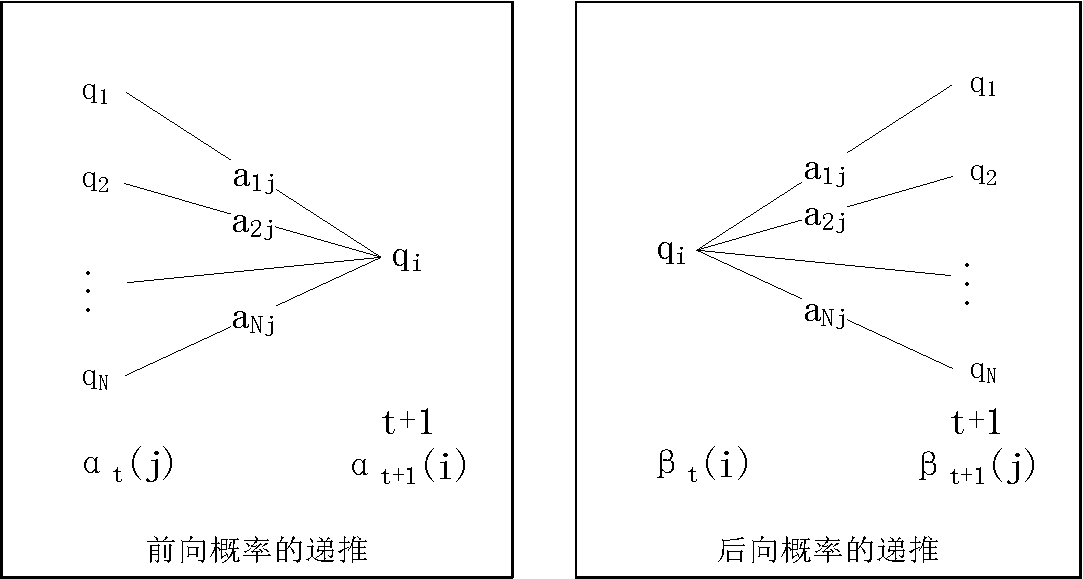
\includegraphics[width=0.9\textwidth]{figures/chapter2/forback-crop}
        \caption{前向后向概率计算示意图}
        \label{fig:forback}
        \end{figure}

        \subsubsection{后向算法}
        \begin{definition}[后向算法]
         给定隐马尔科夫模型$\lambda$,定义在时刻$t$状态为$q_i$的条件下,从$t+1$到$T$的部分观测序列为$({o_{t+1}},{o_{t+2}},\cdots,{o_T})$的概率为后向概率,记作
             \begin{equation}
                 {\beta _t}(i) = P({o_{t + 1}},{o_{t + 2}}, \cdots ,{o_T}|{i_t} = {q_i},\lambda )
             \end{equation}
        \end{definition}

        则可递推地求得后向概率${\beta _t}(i)$及观测序列概率$P(O|\lambda )$,算法描述如下:
        \begin{enumerate}
            \item 初值
                \begin{equation}
                    {\beta _T}(i) = 1,i = 1,2, \cdots ,N
                \end{equation}
            \item 后向递推,对于$t = T - 1,T - 2, \cdots ,1$,如图\ref{fig:forback},
                 \begin{equation}
                    {\beta _t}(i) = \sum\limits_{j = 1}^N {{a_{ij}}{b_j}({o_{t + 1}}){\beta _{t + 1}}(j),i = 1,2, \cdots N}
                 \end{equation}
            \item 终止
                \begin{equation}
                    P(O|\lambda ) = \sum\limits_{i = 1}^N {{\pi _i}{b_i}({o_1}){\beta _1}\left( i \right)}
                \end{equation}
        \end{enumerate}

        \subsubsection{新数学符号定义}
        利用前向概率和后巷概率,我们引出以下概念
        \begin{enumerate}
            \item 观测序列概率$P(O|\lambda )$的统一形式:
                \begin{equation}
                    P(O|\lambda ) = \sum\limits_{i = 1}^N {\sum\limits_{j = 1}^N {{\alpha _t}(i)} {a_{ij}}{b_j}({o_{t + 1}}){\beta _{t + 1}}\left( j \right),} t = 1,2, \cdots T - 1
                \end{equation}
            \item 给定模型$\lambda $和观测$O$,在时刻$t$处于状态$q_i$的概率,记
                \begin{equation}
                    {\gamma _t}(i) = P({i_t} = {q_i}|O,\lambda )
                \end{equation}
                可以通过前向后向概率计算。事实上,
                \[{\gamma _t}(i) = P({i_t} = {q_i}|O,\lambda ) = \frac{{P({i_t} = {q_i},O|\lambda )}}{{P(O|\lambda )}}\]
                由前向后向概率定义可知:
                \[{\alpha _t}(i){\beta _t}(i) = P({i_t} = {q_i},O|\lambda )\]
                如图\ref{fig:gamma},于是有:
                \begin{equation}\label{equation:gamma}
                {\gamma _t}(i) = \frac{{{\alpha _t}(i){\beta _t}(i)}}{{P(O|\lambda )}} = \frac{{{\alpha _t}(i){\beta _t}(i)}}{{\sum\limits_{j = 1}^N {{\alpha _t}(j){\beta _t}(j)} }}
                \end{equation}

                \begin{figure}
                \centering
                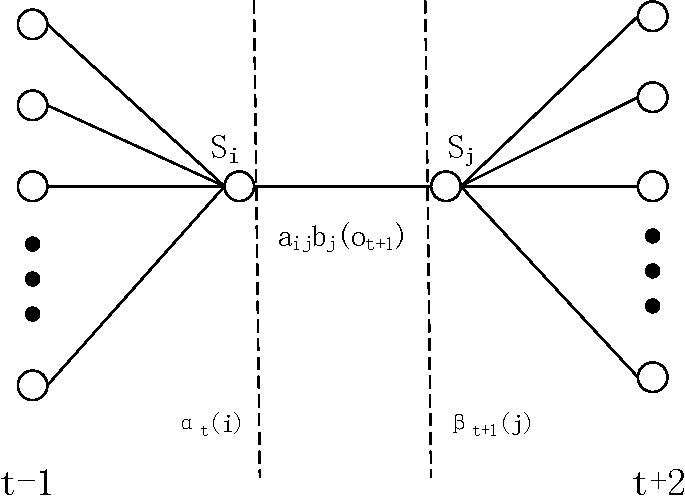
\includegraphics[width=0.7\textwidth]{figures/chapter2/gamma-crop}
                \caption{${\gamma _t}(i)$计算示意图}
                \label{fig:gamma}
                \end{figure}

            \item 定模型$\lambda $和观测$O$,在时刻$t$处于状态$q_i$且在$t+1$时刻处于状态$q_j$的概率记作
                \begin{equation}
                    {\xi _t}(i,j) = P({i_t} = {q_i},{i_{t + 1}} = {q_j}|O,\lambda )
                \end{equation}
                通过前向后向概率计算得:
                \[{\xi _t}(i,j) = \frac{{P({i_t} = {q_i},{i_{t + 1}} = {q_j},O|\lambda )}}{{P(O|\lambda )}} = \frac{{P({i_t} = {q_i},{i_{t + 1}} = {q_j},O|\lambda )}}{{\sum\limits_{i = 1}^N {\sum\limits_{j = 1}^N {P({i_t} = {q_i},{i_{t + 1}} = {q_j},O|\lambda )} } }}\]
                而
                \[P({i_t} = {q_i},{i_{t + 1}} = {q_j},O|\lambda ) = {\alpha _t}(i){a_{ij}}{b_j}({o_{t + 1}}){\beta _{t + 1}}(j)\]
                所以
                \begin{equation}\label{equation:xi}
                {\xi _t}(i,j) = \frac{{{\alpha _t}(i){a_{ij}}{b_j}({o_{t + 1}}){\beta _{t + 1}}(j)}}{{\sum\limits_{i = 1}^N {\sum\limits_{j = 1}^N {{\alpha _t}(i){a_{ij}}{b_j}({o_{t + 1}}){\beta _{t + 1}}(j)} } }}
                \end{equation}
        \end{enumerate}
    \subsection{学习问题}\label{section:learn}
        假设给定训练数据只包含$S$个长度为T的观测序列$\{ {O_1},{O_2}, \cdots ,{O_s}\} $而没有对应的状态序列,目标是学习隐马尔科夫模型$\lambda  = \left( {A,B,\pi } \right)$的参数。我们将观测序列数据看做观测数据$O$,状态序列数据看作不可观测的隐数据$I$,那么隐马尔科夫模型事实上是一个含有隐变量的概率
        模型
        \begin{equation}
        P(O|\lambda ) = \sum\limits_I {P(O|I,\lambda )P(I|\lambda )}
        \end{equation}
        它的学习参数学习可以由EM算法实现。

        EM\ucite{dempster1977maximum}算法是一种迭代算法,1977年由Dempster等人总结提出,用于含有隐变量的概率模型参数的极大似然估计,或极大后验估计。
        EM算法每次迭代由两步组成:E步,求期望
        (Expectation);M步,求极大(Maximization)。
        所以这一算法称为期望极大算法(Expectation Maximization Algorithm),简称EM算法。
        Baum-Welch算法由Baum和Welch提出,是EM算法在隐马尔科夫模型学习中的具体实现。

        下面描述Baum-Welch算法的具体过程。

        Baum-Welch算法输入为观测数据$O = \{ {o_1},{o_2}, \cdots ,{o_T}\}$,输出为隐马尔科夫模型参数。算法步骤如下:
        \begin{enumerate}
            \item 初始化,
                对于$n=0$,选取$a_{ij}^{(0)}$,${b_j}{(k)^{(0)}}$,$\pi _i^{(0)}$,得到模型${\lambda ^{(0)}} = \left( {{A^{(0)}},{B^{(0)}},{\pi ^{(0)}}} \right)$。
            \item 递推,对于$n = 1,2, \cdots $,
                    \[a_{ij}^{(n + 1)} = \frac{{\sum\limits_{t = 1}^{T - 1} {{\xi _t}(i,j)} }}{{\sum\limits_{t = 1}^{T - 1} {{\gamma _t}(i)} }}\]
                    \[{b_j}{(k)^{(n + 1)}} = \frac{{\sum\limits_{t = 1,{o_t} = {v_k}}^T {{\gamma _t}(j)} }}{{\sum\limits_{t = 1}^T {{\gamma _t}(j)} }}\]
                    \[\pi _i^{(n + 1)} = {\gamma _1}(i)\]
                    右端各值按观测$O = \{ {o_1},{o_2}, \cdots ,{o_T}\}$和模型${\lambda ^{(n)}} = \left( {{A^{(n)}},{B^{(n)}},{\pi ^{(n)}}} \right)$计算。
                    式中${{\gamma _t}(j)}$和${{\xi _t}(i,j)}$由式\ref{equation:gamma}和式\ref{equation:xi}给出。
            \item 终止。得到模型参数${\lambda ^{(n + 1)}} = \left( {{A^{(n + 1)}},{B^{(n + 1)}},{\pi ^{(n + 1)}}} \right)$。
        \end{enumerate}

    \subsection{预测问题}\label{section:predict}
    隐马尔科夫模型的预测问题可以由维特比算法(Viterbi算法)解决,下面给出维特比算法。

    维特比算法实际是用动态规划解隐马尔科夫模型预测问题,即用动态规划求最大概率路径(最优路径)。这时求解出的一条路径对应一个状态序列。

    根据动态规划原理,最优路径具有这样的特性;如果最优路径在时刻$t$通过节点${i_t}^*$,那么这一路径从节点${i_t}^*$到终点${i_T}^*$的部分路径,
    对于从${i_t}^*$到${i_T}^*$的所有可能的部分路径来说,必须是最优的。因为如果不是这样,那么从${i_t}^*$到${i_T}^*$就有另一条更好的部分路径
    存在,如果把它和从${i_1}^*$到达${i_t}^*$的部分路径连接起来,就会形成比原来路径更优的路径,这是矛盾的。依据这一原理,我们只需从$t=1$时刻
    开始,递推地计算在时刻$t$状态为$i$的各条部分路径的最大概率,直至得到时刻$t=T$状态为$i$的各条路径的最大概率。时刻$t=T$的最大概率即为最大
    概率即为最有路径的概率${P^*}$,最优路径的终结点${i_T}^*$也同时得到。之后,为了找出最优路径的各个节点,从终结点${i_T}^*$开始,由后向前逐步
    求得节点${i_{T - 1}}^*, \cdots ,{i_1}^*$,得到最优路径${I^*} = ({i_1}^*,{i_2}^*, \cdots ,{i_{T - 1}}^*,{i_T}^*)$,这就是维特比算法。

    算法首先导入两个变量$\delta $和$\psi $。定义在时刻$t$状态为$i$的所有单个路径$({i_1},{i_2}, \cdots ,{i_t})$中概率最大值为
        \begin{equation}
            {\delta _t}(i) = \mathop {\max }\limits_{{i_1},{i_2}, \cdots ,{i_{t - 1}}} P({i_t} = i,{i_{t - 1}}, \cdots ,{i_1},{o_t}, \cdots ,{o_1}|\lambda ),i = 1,2,, \cdots ,N
        \end{equation}

    由定义可得变量$\delta $的递推公式:
        \begin{equation}
            \begin{array}{l}
            {\delta _{t + 1}}(i) = \mathop {\max }\limits_{{i_1},{i_2}, \cdots ,{i_t}} P({i_{t + 1}} = i,{i_t}, \cdots ,{i_1},{o_{t + 1}}, \cdots ,{o_1}|\lambda )\\
            \;\;\;\;\;\;\;\;\; = \mathop {\max }\limits_{1 \le j \le N} \left[ {{\delta _t}(j){a_{ji}}} \right]{b_i}({o_{t + 1}}),i = 1,2, \cdots ,N;t = 1,2, \cdots,T - 1
        \end{array}
        \end{equation}

    定义在时刻$t$状态为$i$的所有单个路径$({i_1},{i_2}, \cdots ,{i_t})$中概率最大的路径第$t-1$个节点为:
         \begin{equation}
            {\psi _t}(i) = arg\mathop {\max }\limits_{1 \le j \le N} [{\delta _{t - 1}}(j){a_{ji}}],i = 1,2, \cdots, N
        \end{equation}

    下面描述Viterbi算法的具体过程。

    算法输入为观测数据$O = \{ {o_1},{o_2}, \cdots ,{o_T}\}$和模型参数$\lambda  = \left( {A,B,\pi } \right)$,输出为最优路径${I^*} = ({i_1}^*,{i_2}^*, \cdots ,{i_{T - 1}}^*,{i_T}^*)$。算法步骤如下:
    \begin{enumerate}
        \item 初始化
            \[{\delta _1}(i) = {\pi _i}{b_i}({o_1}),i = 1,2, \cdots ,N\]
            \[{\psi _1}(i) = 0,i = 1,2, \cdots ,N\]
        \item 递推,对于$t = 1,2, \cdots,T$,
            \[{\delta _t}(i) = \mathop {\max }\limits_{1 \le j \le N} \left[ {{\delta _{t - 1}}(j){a_{ji}}} \right]{b_i}({o_t}),i = 1,2, \cdots ,N\]
            \[{\psi _t}(i) = arg\mathop {\max }\limits_{1 \le j \le N} [{\delta _{t - 1}}(j){a_{ji}}],i = 1,2, \cdots ,N\]
        \item 终止
             \[{P^*} = \mathop {\max }\limits_{1 \le i \le N} {\delta _T}(i)\]
             \[{i_T}^* = arg\mathop {\max }\limits_{1 \le i \le N} \left[ {{\delta _T}(i)} \right]\]
        \item 最优路径回溯。对于$t = T-1,T-2, \cdots,1$
            \[{i_t}^* = {\psi _{t + 1}}({i_{t + 1}}^*)\]
            从而求得最优路径${I^*} = ({i_1}^*,{i_2}^*, \cdots ,{i_{T - 1}}^*,{i_T}^*)$
    \end{enumerate}



\section{连续密度的隐马尔科夫模型}

    以上讨论中,我们都假定观测输出概率,也就是$B$参数的分布是离散的,本节介绍连续密度的隐马尔科夫模型(Continuous HMM,CHMM)。
    在连续密度隐马尔科夫模型中,观测输出概率是连续的,而不是有限的,所以不能用观测矩阵来表示输出概率,而要改用概率密度函数来表示。
    假设$\bm{X}$为观测向量,则$[b_{j}(\bm{X})d\bm{X}]$表示在$\bm{X}$和$\bm{X}+d\bm{X}$之间观察矢量的输出概率。这里$b_{j}(\bm{X})$
    称为参数$\bm{X}$的概率密度分布函数,输出$\bm{X}$的概率可以通过$b_{j}(\bm{X})$计算。$b_{j}(\bm{X})$一般用高斯概率密度函数,由于
    $\bm{X}$是多维矢量,所以要用多元高斯密度函数,如式\ref{equation:gm}所示。
    \begin{equation}\label{equation:gm}
       {b_j}(\bm{X}) = \frac{1}{{{{(2\pi )}^{p/2}}{|{\bm{\Sigma}} |_j^{ - 1}}}}\exp \left\{ { - \frac{1}{2}(\bm{X} - {{\bm{\mu}} _j}) {\bm{\Sigma}}_j^{ - 1}{{(\bm{X} - {{\bm{\mu}}_j})}^T}} \right\}
    \end{equation}

    另一方面,在实际应用中,仅用一个高斯概率密度函数不足以表述语音参数$\bm{X}$的输出概率分布,所以常用多个高斯函数的叠加组合来表示输出概率
    密度函数,称为混合高斯模型,如式\ref{equation:gmm}所示。
    \begin{equation}\label{equation:gmm}
       {b_j}(\bm{X}) = \sum\limits_{m = 1}^M {{\omega _{jm}}} \frac{1}{{{{(2\pi )}^{p/2}}|{\bm{\Sigma}} |_{jm}^{ - 1}}}\exp \left\{ { - \frac{1}{2}(\bm{X} - {{\bm{\mu}} _{jm}}){\bm{\Sigma}}_{jm}^{ - 1}{{(\bm{X} - {{\bm{\mu}} _{jm}})}^T}} \right\}
    \end{equation}

    其中$M$表示混合高斯数,即使用$M$个高斯叠加组合描述输出概率密度函数,${\omega_{jm}}$是混合系数,表示第$m$个高斯所占权重。混合高斯的引入,极大的增强了模型
    的描述能力。


\section{HMM在语音识别中的应用}
    结合HMM的三个基本问题和连续密度的HMM,本节介绍HMM在语音识别中的模型建立、训练过程和识别过程的基本应用。

    首先,要明确在语音识别任务中观测是什么、状态是什么。观测是人所发出的一段语音信号,人在说不同词时会产生不同的语音信号,不同的语音信号对应不同的信号特征(
    如幅度、频率、过零率等),我们对语音信号进行特征提取,即可作为HMM模型的观测向量。人在发出不同音素时对应不同的发音过程,状态即是对不同发音过程的描述。
    由于人的发音过程不可逆,即状态跳转不可逆,语音识别任务中使用特殊的HMM模型,称为左右模型,如图\ref{fig:left_right}所示,可以看出仅能跳转到
    自身或更高的状态。若以音素为基本单位建立HMM模型,则一般使用3状态的HMM描述,如图\ref{fig:asr_hmm}所示,其中1、5状态为扩展状态,1状态为起始状态,只能跳转到其它
    状态;5状态为结束状态。1、5状态均不产生任何观测输出,只是为了描述的方便,特别在HMM模型连接中非常有用。

    \begin{figure}
    \centering
    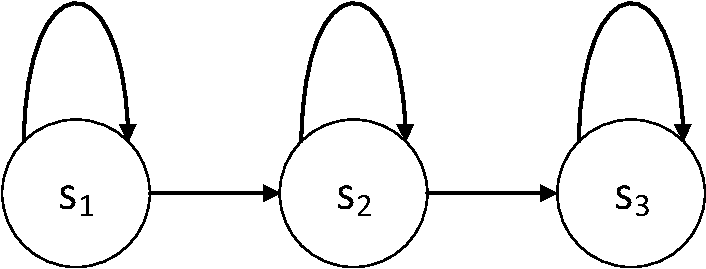
\includegraphics[width=0.5\textwidth]{figures/chapter2/left_right-crop}
    \caption{左右模型HMM}
    \label{fig:left_right}
    \end{figure}

    \begin{figure}
    \centering
    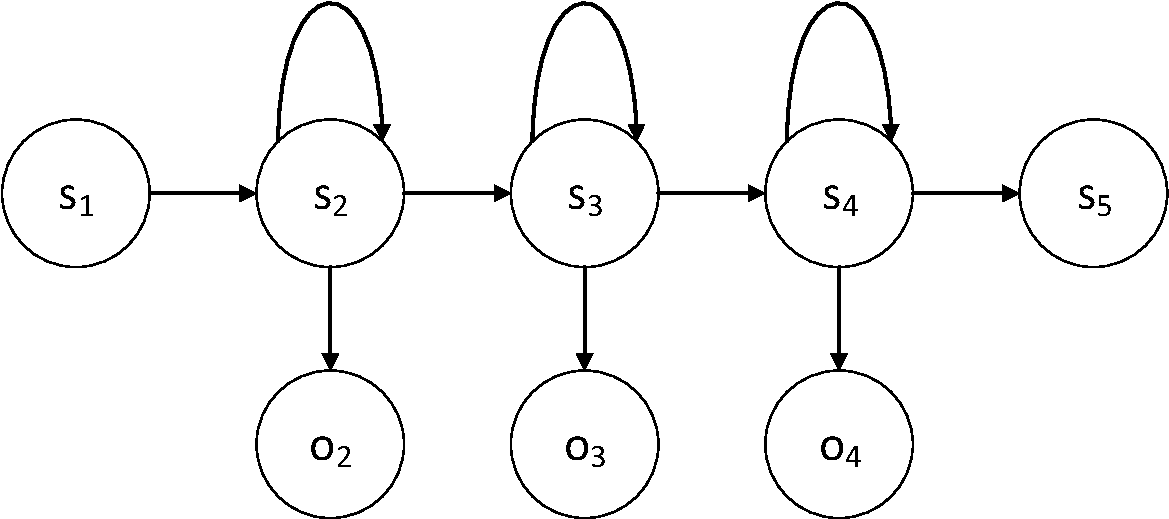
\includegraphics[width=0.8\textwidth]{figures/chapter2/asr_hmm-crop}
    \caption{语音识别中的5状态HMM}
    \label{fig:asr_hmm}
    \end{figure}

    模型的训练是一个不断迭代的过程,目的是求得各个HMM模型的参数。以音素为基本单位的训练过程如下:
    首先,对每个音素建立一个HMM模型,并对模型参数$\lambda $进行初始化。
    每一轮的训练过程中,根据HMM模型参数,先使用前向后向算法计算(HMM概率问题\ref{section:probability})在所有时间$t$上的前向得分和后向得分,随后进行Baum-Welch
    算法(HMM学习问题\ref{section:learn})对模型参数进行更新,其中E步计算观测下各状态出现、各状态转移、由状态$i$转移到状态$j$的期望,并计算混合高斯分量权重的期望,
    M步对状态转移矩阵,各状态概率密度函数混合高斯的均值、协方差矩阵参数进行更新。
    重复进行训练过程,直至满足预设条件终止。

    在已经得到各个HMM的模型参数后,识别过程就是计算给定观测在不同HMM模型上的概率,选取概率最大HMM模型对应的状态序列即为识别结果,也就是使用Viterbi算法(HMM预测问题\ref{section:predict})。
    在大词汇量连续语音识别中,为了提高解码效率,会采取一定的剪枝策略,如Beam Search等。

%\section{基于HTK的连续语音识别系统}
%    \subsection{HTK工具包介绍}
%
%    HTK(HMM Tools Kit)\cite{young1997htk}是一个剑桥大学开发的专门用于建立和处理HMM的实验工具包,主要应用于语音识别领域,也可以应用于语音合成、字符识别和
%    DNA排序等领域。HTK经过剑桥大学、Entropic公司及Microsoft公司的不断增强和改进,使其在世界范围内得到广泛应用。并且,HTK源代码开放,
%    基于ANSI C实现,所以具有良好可移植性和跨平台性。HTK由库程序和工具程序两部分组成。库程序提供一系列函数和接口;工具程序为语音分析,
%    HMM训练、测试和结果分析提供一系列实现。
%
%    其中本毕设中主要使用HTK核心模块HEREST(训练工具)和HVite(识别工具)。
%
%
%    \subsection{HTK连续语音识别系统搭建}
%    \begin{figure}[h]
%        \centering
%        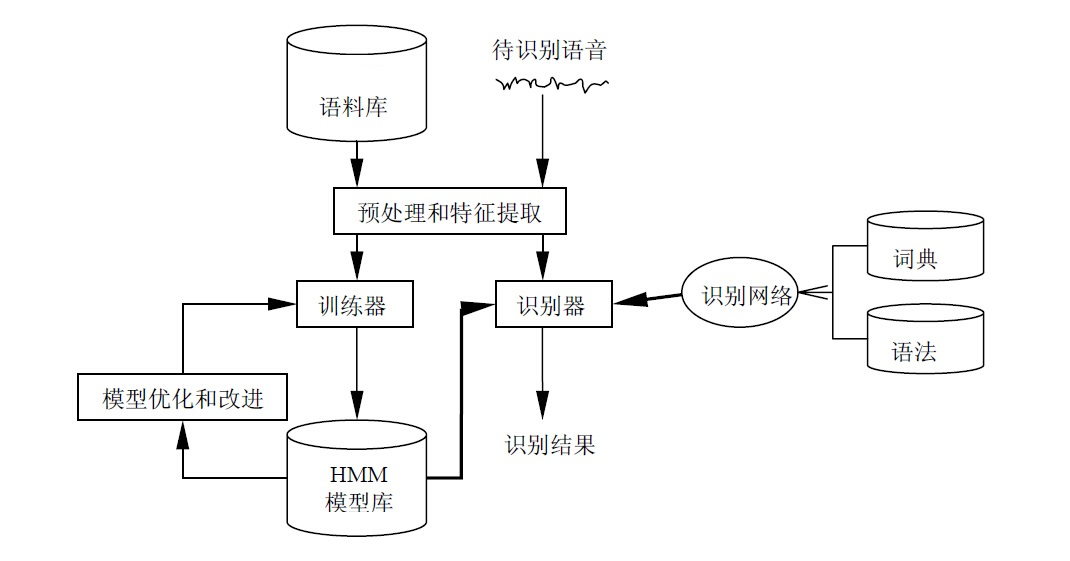
\includegraphics[width=0.8\textwidth]{figures/chapter2/asr_system}
%        \caption{连续语音识别系统框架}
%        \label{fig:asr_system}
%    \end{figure}
%
%    一个连续语音识别系统架构如图\ref{fig:asr_system}所示,由图可以看出,整个系统由训练和识别两大部分组成,在HTK中其对应核心实现部分为HEREST和HVite。
%
%    本节介绍基于HTK连续语音识别系统搭建的数据准备、模型训练和识别系统。
%
%    数据准备部分主要准备字典、词典和语音数据及其对应标注抄本。本毕设中主要依托实验室的资源。
%
%    模型训练过程为:对语音数据进行特征提取;创建单音素模型;加入上下文信息创建三音素模型,三音素模型状态绑定,最后对HMM模型逐步增加混合高斯数。
%    训练过程中重复使用到HEREST。
%
%    识别系统首先定义任务所需的词网络,根据训练过程中产生的模型文件,先对输入语音进行特征提取,然后由识别器词网络在上根据声学模型和语言模型进行打分,进而
%    得到识别结果。识别过程核心为HVite,为了移植HVite到DSP,本毕设对HVite源代码进行了解析。


% !Mode:: "TeX:UTF-8"

\chapter{基于深度学习的声学建模}\label{intro_dl}


深度学习在语音识别中的引入,替代了经典HMM-GMM系统中采用GMM对状态概率密度进行建模的方法,
使用深度神经网络对状态的概率分布进行建模,称之为基于HMM-DNN(HMM-Deep Neural Network)的语音识别系统。

本章介绍深度学习的基本原理及其在语音识别中的基本应用。
首先介绍几种常见的神经网络结构全接连的神经网络DNN、
卷积神经网络CNN、循环神经网络RNN等深度学习网络的基本结构;
然后研究这些深度学习网络在声学模型这个特定任务中的使用方式,改进和组合使用(CLDNN)等;
最后本章给出这几种深度学习方法的相关语音识别实验。

\section{HMM-DNN系统}\label{section:hmmdl}

在经典HMM-GMM的语音识别系统中,为每个状态建立一个GMM模型来描述其概率分布,
在识别时,通过各自状态的GMM可以直接计算$t$时刻的观测$o_t$在状态$s_i$上的概率
$p(o_t|s_i)$,$p(o_t|s_i)$HMM系统识别时必须的依赖。

深度学习引入语音识别后,使用深度神经网络来替代GMM对每个状态进行建模,
在深度神经网络中,这是一个典型的分类任务,即当新的一帧语音到来时,
通过深度神经网络计算其在每个状态上的概率。
与GMM系统为每个状态建立独立的GMM模型不同,深度神经网络本身为紧凑模型,即所有状态共享一个模型。
通过深度神经网络直接计算出的是$p(s_i|o_t)$,而非$p(o_t|s_i)$,
这是基于GMM和神经网络对声学模型进行建模的一个本质上的不同。

通过贝叶斯公式有:
\begin{equation}
p(o_t|s_i) = \frac{p(s_i|o_t)p(o_t)}{p(s_i)}
\end{equation}
在识别的解码过程中,为防止概率连乘导致下溢,概率计算一般转到$log$域,取$log$有:
\begin{equation} \label{equation:hmmdnn}
\begin{array}{l}
\log{p(o_t|s_i)} = \mathop {\log{p(s_i|o_t)} + \log{p(o_t)} - \log{p(s_i)}} \\
\;\;\;\;\;\;\;\;\;\;\;\;\;\;\;\;\; = \mathop {\log{p(s_i|o_t)} - \log{p(s_i)}}
\end{array}
\end{equation}
其中$p(o_t)$为$o_t$发生的概率,对所有的状态相同,因此可以忽略。
$p(s_i)$为状态$s_i$出现的概率,称之为状态先验,一般可以通过对训练数据集作状态统计得到。
通过公式\ref{equation:hmmdnn},便可以计算得到$p(o_t|s_i)$,这是基于HMM-DNN系统进行语音
识别的基本原理。
如图\ref{fig:hmmdnn}所示,原始语音信号经过特征提取,输入到神经网络,
计算当前信号在每个状态上的概率,然后结合该概率在HMM系统中进行语音识别解码。


\begin{figure}[htbp]
\centering
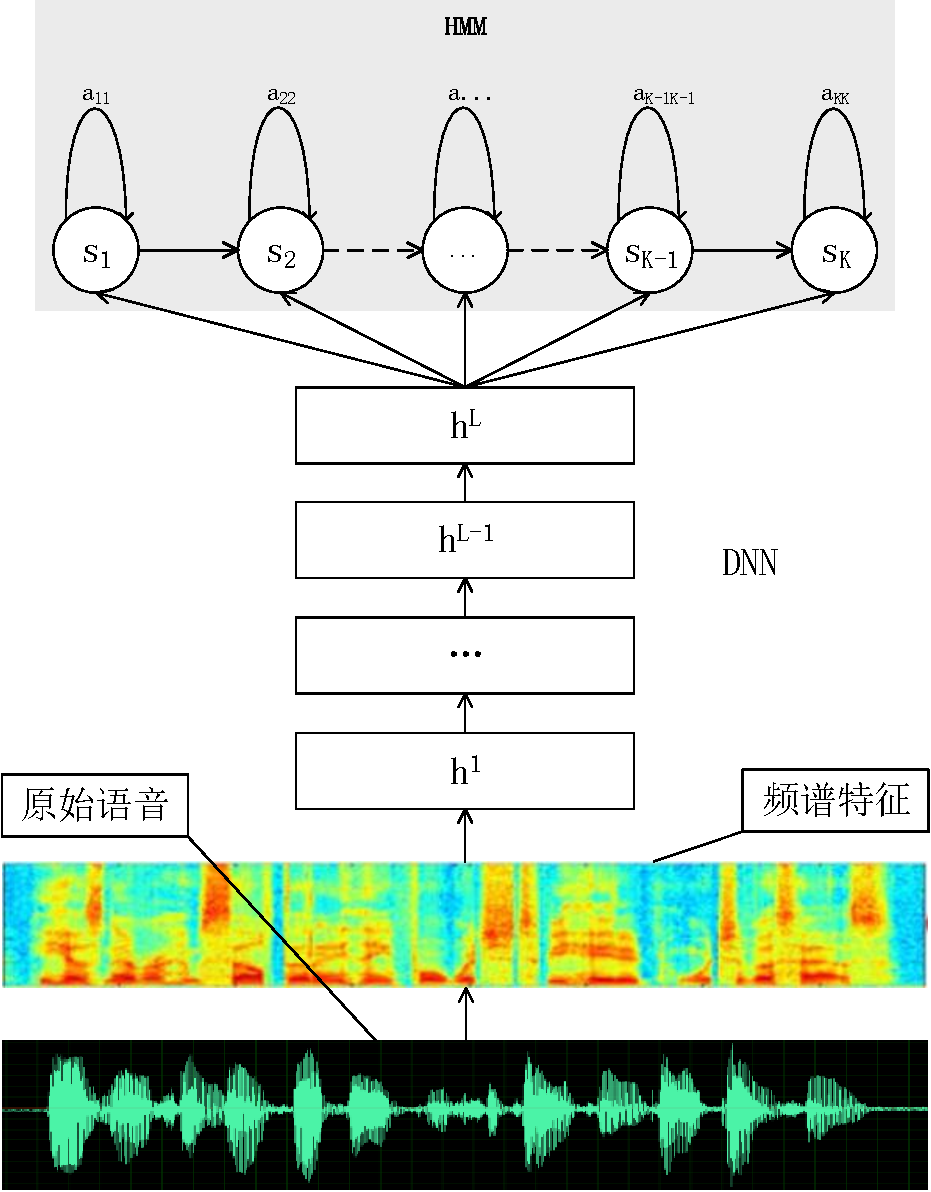
\includegraphics[width=0.5\textwidth]{figures/chapter3/hmmdnn-crop}
\caption{HMM-DNN系统的基本原理}
\label{fig:hmmdnn}
\end{figure}


\section{全连接神经网络DNN}

深度神经网络DNN\ucite{bengio2012practical}(Deep Neural Network)是有多个(一般均大于2层)隐层的传统的多层感知机MLP(Multi-Layer Perceptron)。
一个典型的神经网络由输入层;中间多个隐层和输出层组成。
如图\ref{fig:dnn}所示DNN,含有3个隐层,每个隐层有5个节点。
在一个$L+1$层的DNN中,我们定义输入层为第$0$层,输出层为第$L$层。

\begin{figure}[htbp]
\centering
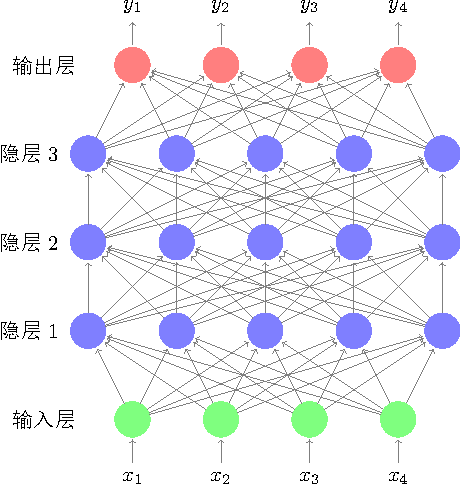
\includegraphics[width=0.5\textwidth]{figures/chapter3/dnn-crop}
\caption{DNN示例(该DNN由输入层、3个隐层和输出层组成)}
\label{fig:dnn}
\end{figure}

对于任意隐层$l$的任意节点$j$,有:
\[\begin{array}{l}
a_j^l = \sum\limits_{i = 1}^N {w_{ji}^l {x_i}^{l-1}+ b_j^l} \\
z_j^l = h(a_j^l)
\end{array}\]
其中,$i = 1,...,N$表示$l-1$层的节点数目,$a_j^l$表示第$l$层第$j$个节点的激励,
$a_j^l$经过激活函数$h(.)$作用得到$z_j^l$。
通常$h(.)$为非线性的、可导函数,
通过非线性函数增强神经网络的非线性映射能力,可导性则可以使神经网络通过梯度的方法行优化。

\subsection{激活函数}

在深度神经网络的实际应用中,最常用的激活函数是$sigmoid$函数:
\begin{equation}
s(z) = \frac{1}{{1 + {e^{ - z}}}}
\end{equation}
或者$tanh$函数:
\begin{equation}
\tanh (z) = \frac{{{e^z} - {e^{ - z}}}}{{{e^z} + {e^{ - z}}}}
\end{equation}
$sigmoid$函数将输入通过非线性函数映射到空间$(0,1)$;$tanh$函数的值域空间为$(-1,1)$,
其映射空间具有对称性。$ReLU$\ucite{glorot2011deep}是近年深度学习技术流行之后,又一个非常有效的激活函数:
\begin{equation} \label{equation:relu}
{\mathop{\rm Re}\nolimits} LU(z) = \max (0,z)
\end{equation}
$ReLU$激活函数预测具有稀疏性,这中预测特性提高了网络的泛化能力;另一方面,
如式\ref{equation:relu},$ReLU$的梯度形式简单,非0即1,有效的缓解了深度神经网络
训练中的梯度弥散问题;而且$ReLU$激活函数的计算更加简单,速度更快。
三种激活函数如图\ref{fig:activation}所示。

\begin{figure}[htbp]
\centering
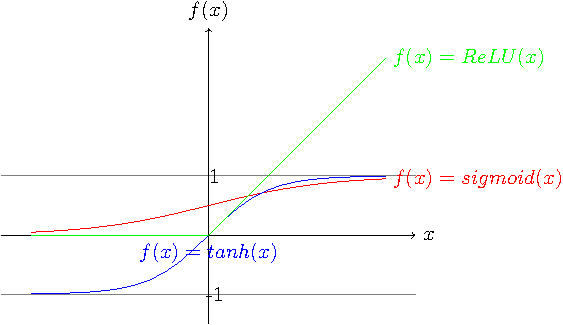
\includegraphics[width=0.6\textwidth]{figures/chapter3/activation-crop}
\caption{激活函数$sigmoid$、$tanh$和$ReLU$对比}
\label{fig:activation}
\end{figure}

激活函数的选择和深度神经网络密切相关,因此设计更好的激活函数也成为当下深度学习研究的热点之一,
最近的实验\ucite{zhang2014improving, zhang2015parameterised}表明,经过精心设计的激活函数能够
在一定程度上提高深度神经网络的性能。

\subsection{DNN训练}

DNN的训练即在损失函数确定后,使用误差方向传播BP(Back Propagation)算法计算参数梯度,
使用随机梯度下降SGD(Stochastic Gradient Descent)对模型中的参数进行更新。

一般来说,对于回归任务,使用最小均方误差MSE(Mean Suqare Error)损失函数:
\begin{equation}
E({\rm{w}}) = \frac{1}{2}\sum\limits_{n = 1}^N {\{ {y_n}}  - {t_n}{\} ^2}
\end{equation}
其中$y_n$为网络输出,$t_n$为标注,$N$为样本总数。

对于分类任务,应用softmax函数:
\begin{equation}
\label{equation:softmax}
{y_k} = \frac{{\exp ({a_k})}}{{\sum\limits_j {\exp ({a_{\rm{j}}})} }}
\end{equation}
计算在每个类别上的归一化后的概率,然后使用交叉熵CE(Cross Entropy)准则计算损失:
\begin{equation}
E(w) =  - \sum\limits_{n = 1}^N {\sum\limits_{k = 1}^K {{t_{kn}}\ln {y_k}} }
\end{equation}

根据\ref{section:hmmdl},基于深度神经网络的声学建模为典型的分类任务,
在输出层使用$softmax$函数做概率归一,使用交叉熵作为损失函数。

\section{卷积神经网络}

CNN最早应用在图像领域,在基础DNN的结构上,CNN引进了局部滤波器,池化层和权值共享三个新思想。
深度学习在语音识别领域获得成功后,研究人员开始探索CNN在语音识别任务上的应用。

语音信号在频域上具有一定的局部特性,不同的音素在不同的局部频带上能量比较集中。
例如,非静音的音素在不同频带上有一定的共振峰。
在这些频带上应用局部滤波器或许能够提供对这些局部特征结构的更有效的表示,
这个特点是CNN能够应用在语音识别任务上的基础。

在语音识别中,CNN中使用卷积层能够对局部频域特征建模。
将输入语音信号分频带规整好之后,卷积层中每个卷积核的输入都为一定频段的语音信号。
假设输入信号$\textbf{x}$被分为$N$个频带$\textbf{x}= [\textbf{x}_1, \textbf{x}_2, ..., \textbf{x}_N]$,
其中向量$\textbf{x}_n$代表频段$n$。如图\ref{fig:cnn}所示,这个$\textbf{x}_n$可以包含原始频谱,一阶差分和二阶差分。
卷积层的激励被分为$K$个子带,每个频带包含$J$个滤波器的激励。
将每个子带的激励记作$\textbf{q}_k$ = $[q_{k,1}, q_{k,2}, ..., q_{k, J}]$,则有:
\begin{equation}
{{\rm{q}}_{k,j}} = h(\sum\limits_{n = 1}^{s - 1} {{\textbf{w}_{n,j}}\textbf{x}_{n{\rm{ + k}}}^T + {b_j})}
\end{equation}
其中,$h(.)$表示激活函数,$s$表示局部滤波器的宽度,$\textbf{w}_{n,j}$表示第$j$个滤波器的的第$n$维权重向量。


\begin{figure}[htbp]
\centering
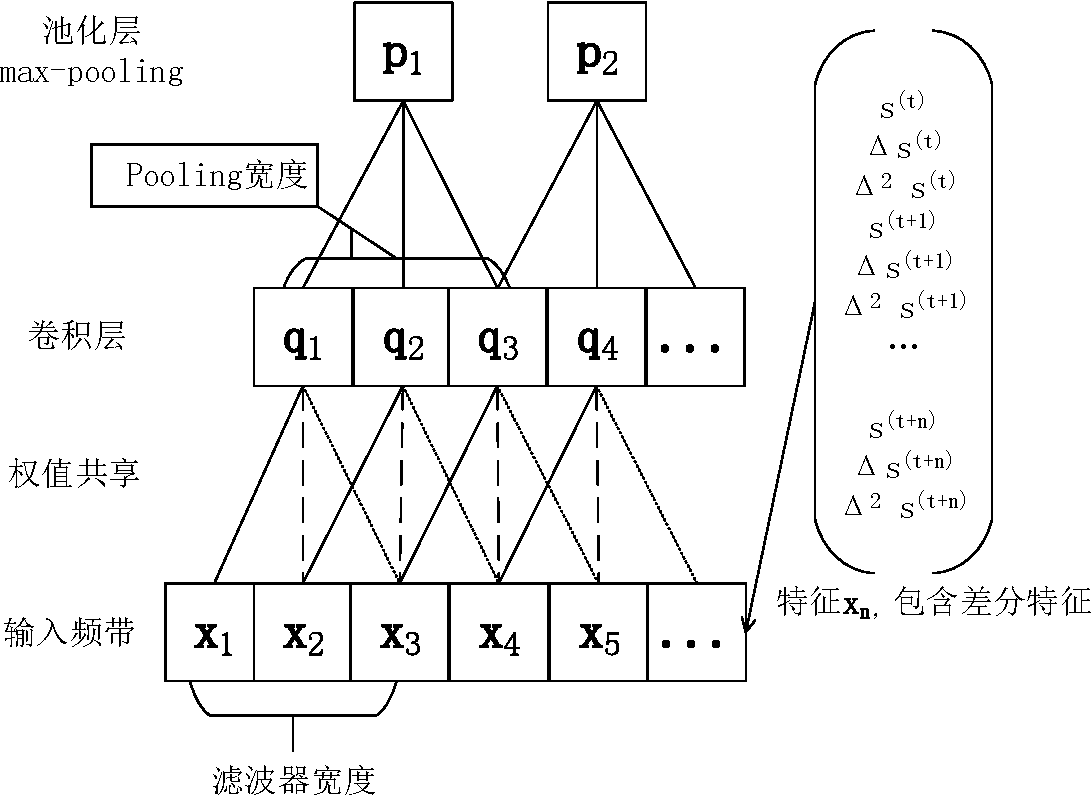
\includegraphics[width=0.6\textwidth]{figures/chapter3/cnn-crop}
\caption{CNN基本结构示意}
\label{fig:cnn}
\end{figure}

在CNN中,使用max-pooling(最大池化层)来保证局部不变性,max-pooling层一般位于卷积层之后,
作用在卷积层的激励输出上。max-pooling通过对局部激励取最大(max)操作,从而得到低分辨率的卷积层的输出,
这种表示更为抽象,更为鲁棒,随后作为高层神经网络的输入处理。
假设max-pooling操作共产生$M$个子带,将第$m$个子带的激励记作
$\textbf{p}_m$ = $[p_{m,1}, q_{m,2}, ..., q_{m, J}]$,则有:
\begin{equation}
{p_{m,j}} = \mathop {\max }\limits_{k = 1}^r ({q_{m \times n + k,j}})
\end{equation}
其中,$r$是pooling的大小,$n$是pooling的步长,一般小于$r$(这样允许临近的pooling操作可以有重叠),
图\ref{fig:cnn}中,pooling的大小为3,步长为2.

基于CNN的语音识别网络如图\ref{fig:cnnasr}所示。如上分析,CNN的输入为频域特征,
Fbank(Filter bank)特征是目前最为常用的频谱特征。
神经网络的底层为一层或者多层的CNN,用作频谱特征的抽取,之后会连接普通的DNN神经网络。
基于CNN的语音识别也是目前识别领域的研究热点之一,
一种趋势是直接CNN直接对原始音频Raw进行建模\ucite{palaz2015convolutional, sainath2016factored},
另一种趋势应用已经在图像上应用获得成功的Deep CNN\ucite{yu2016deep, xiong2016microsoft, sercu2016very, saon2015ibm}的结构到语音识别任务中。


\begin{figure}[htbp]
\centering
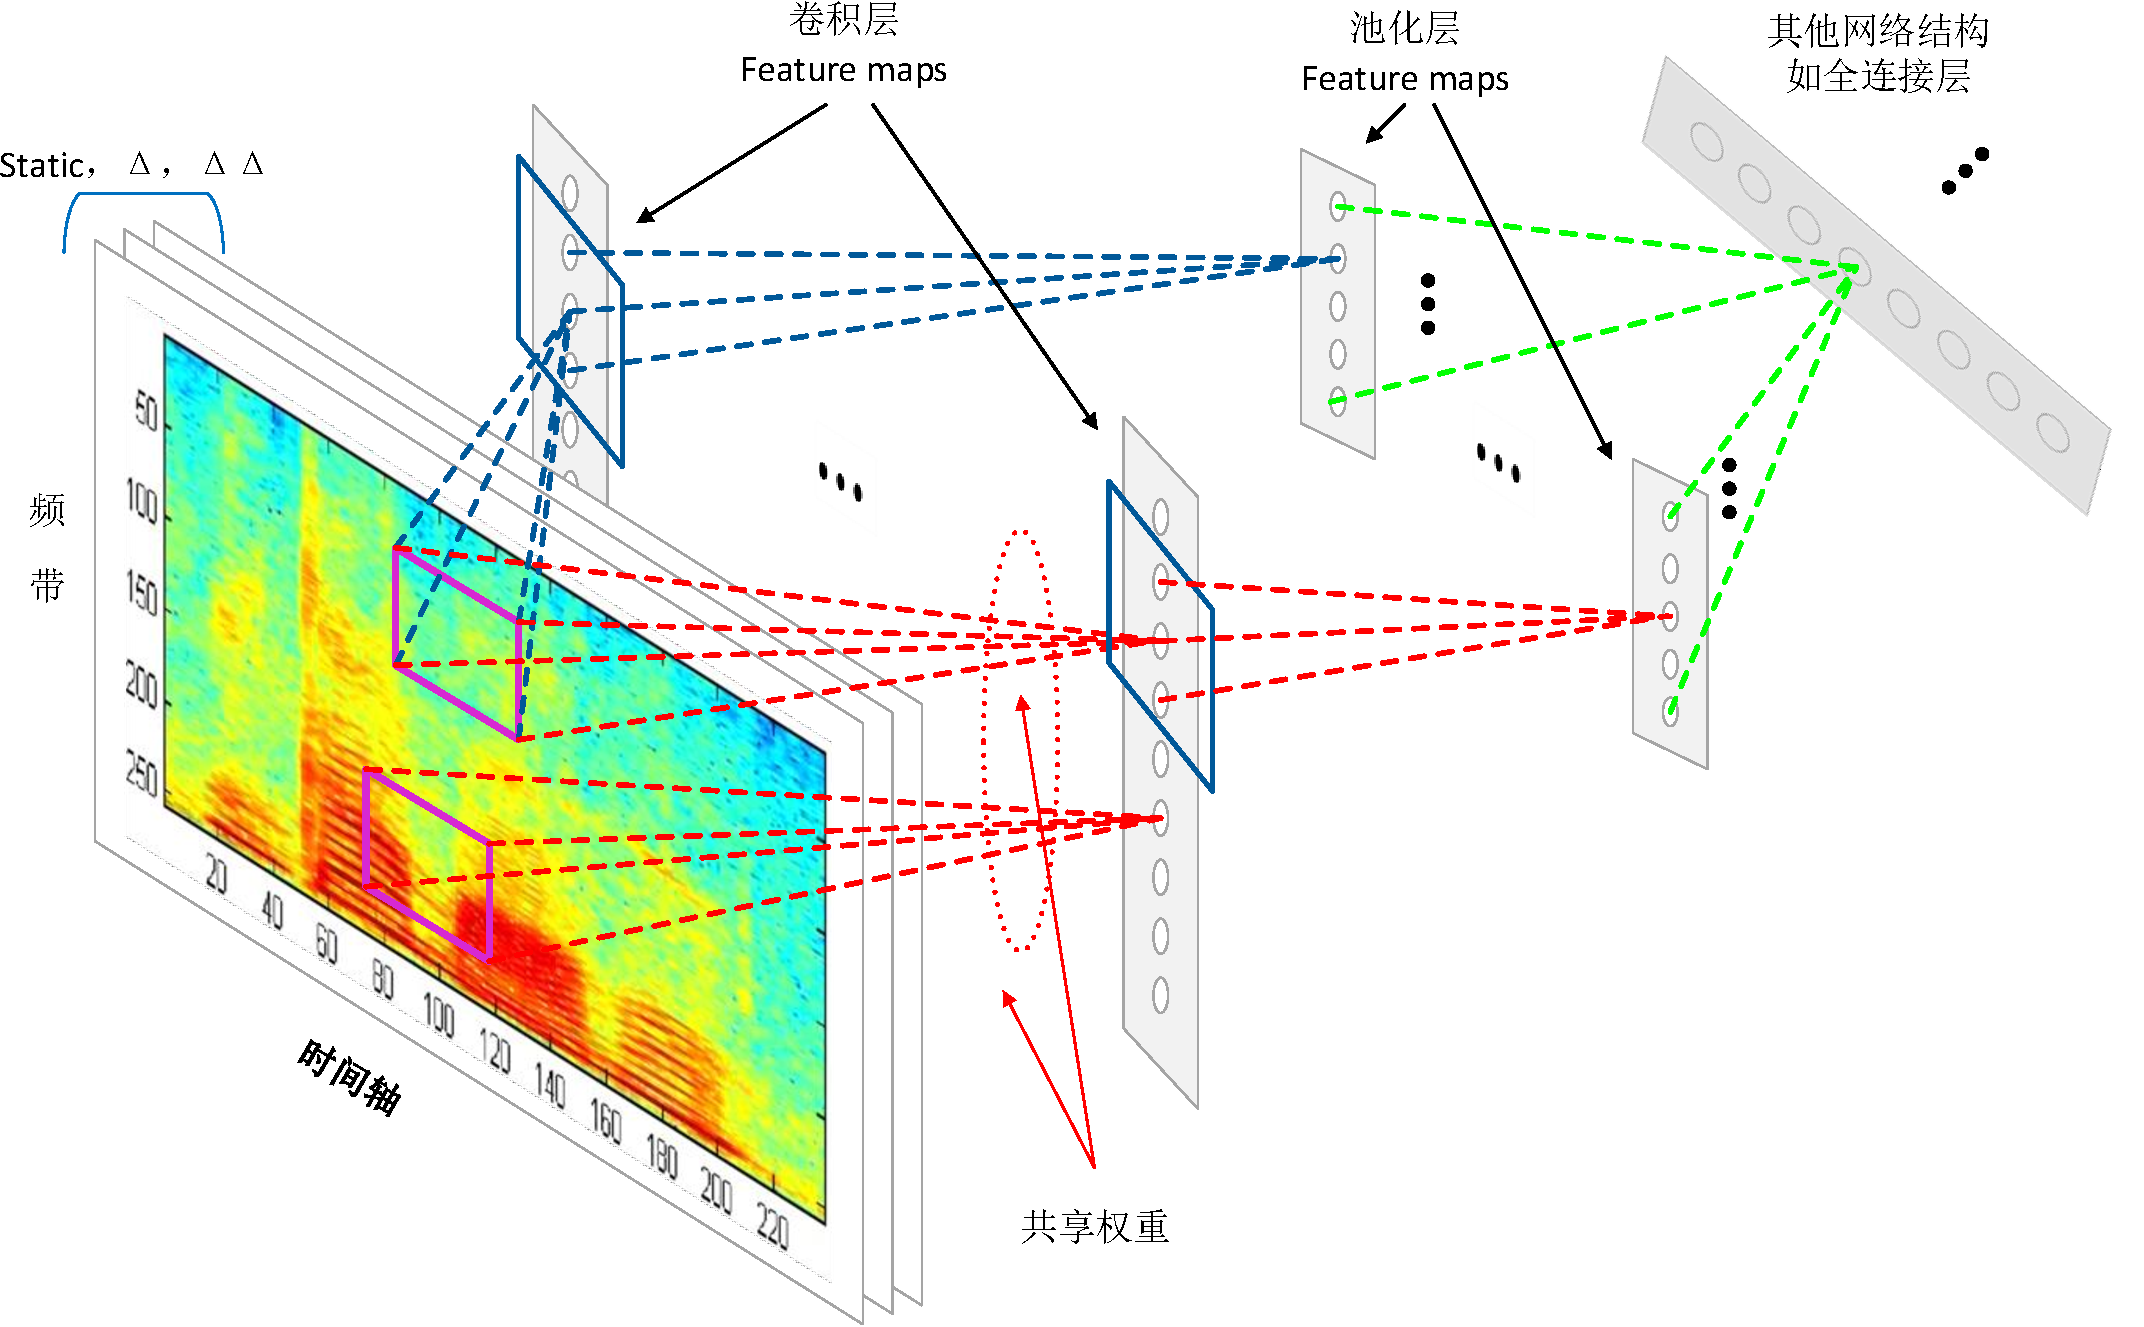
\includegraphics[width=0.8\textwidth]{figures/chapter3/cnnasr-crop}
\caption{基于CNN的声学模型}
\label{fig:cnnasr}
\end{figure}

\section{循环神经网络}

循环神经网络RNN是一种带有Recurrent层的神经网络,循环Recurrent层中的神经元通过连接组成了一个有向环,
有向环使得循环神经网络有了内部状态和记忆单元的结构,从而赋予了循环神经网络记忆功能和对时序动态建模的能力。
如图\ref{fig:rnn}所示,循环神经网络RNN中循环层与全连接层的不同之处在于RNN的输出不仅是当前时刻下一层的输入,
同时还有上一时刻该循环层的输出,通过这样的结构,RNN能够在内部表示和学习序列中的历史信息。

语音识别任务是天然的时序序列标注任务,即把一段语音数据识别为相应的文本序列,
这是RNN能够成功应用在语音识别任务的基础。

RNN有许多变种的结构,这里我们介绍简单循环神经网络(记为RNN)和当前最为流行的长短时记忆(LSTM)的循环神经网络。


\begin{figure}[htbp]
\centering
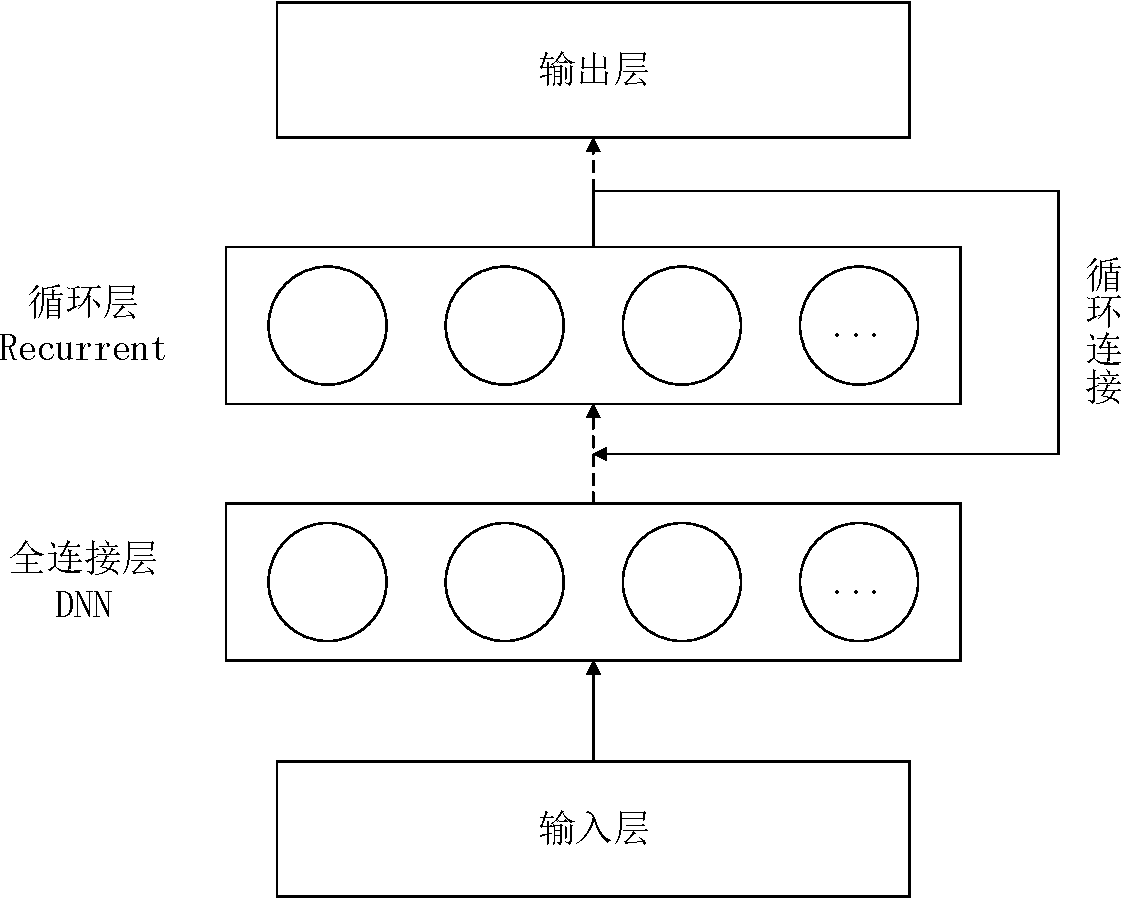
\includegraphics[width=0.5\textwidth]{figures/chapter3/rnn-crop}
\caption{循环神经网络RNN的基本结构}
\label{fig:rnn}
\end{figure}

\subsection{简单循环神经网络}

简单循环神经网络RNN的结构和图\ref{fig:rnn}所示相同。
在任意时刻$t$,使用$\textbf{x}_t$表示前一层的$M$维输出,$\textbf{h}_t$是$N$维的隐状态向量,
则循环层RNN的输出可以表示为:
\begin{equation}
\textbf{h}_t = f({\textbf{W}_{xh}}{\textbf{x}_t} + {\textbf{W}_{hh}}{\textbf{h}_{t-1}})
\end{equation}
其中$f(.)$表示激活函数, $\textbf{W}_{xh}$是$N \times M$的连接前一层的权值矩阵,
$\textbf{W}_{hh}$是$N \times N$的连接$t-1$时刻该循环层输出$\textbf{h}_{t-1}$的权值矩阵,
$\textbf{h}_{t-1}$即是RNN的内部状态。

\subsection{长短时记忆}

RNN的结构相对简单,具有一定的对序列、时间轨迹建模能力,但在序列长度更大、问题更为复杂的任务中,
其建模能力则十分有限;此外,简单RNN的训练容易出现梯度爆炸或者弥散的问题,训练不够稳定。

为了解决上述问题,1997年,Hochreiter等人提出了LSTM\ucite{hochreiter1997long},
LSTM通过引入门结构复杂化RNN的基本结构,强化了建模能力;通过引入CEC(Constant Error Carousel)单元解决RNN训练中的不稳定问题。


LSTM的基本结构如图\ref{fig:lstm}左图所示,它的基本思想是利用不同类型的门来控制网络中的信息流。
LSTM结构中含有输入门、输出门、遗忘门三种基本门结构,门的基本输入为网络上一层的输出和该Recurrent层上一时刻的输出;
同时LSTM结构中引入cell单元,cell单元和隐层输出一起作用强化RNN的记忆功能。
LSTM的数据流向如下:
\begin{equation}
\begin{array}{l}
{{\rm{i}}_t} = \sigma ({W_{ix}}{x_t} + {W_{ih}}{h_{t - 1}}{\rm{ + }}{b_i})\\
{f_t} = \sigma ({W_{fx}}{x_t} + {W_{fh}}{h_{t - 1}}{\rm{ + }}{b_f})\\
{o_t} = \sigma ({W_{ox}}{x_t} + {W_{oh}}{h_{t - 1}}{\rm{ + }}{b_o})\\
{c_t} = {f_t} \odot {c_{t - 1}} + {i_t} \odot \tanh ({W_{cx}}{x_t} + {W_{ch}}{h_{t - 1}}{\rm{ + }}{b_c})\\
{h_t} = {o_t} \odot \tanh ({c_t})
\end{array}
\end{equation}
其中$i_t$表示输入门,$f_t$表示遗忘门,$o_t$表示输出门;$c_t$表示cell的内部值;
$\sigma$表示sigmoid激活函数;
$W$均为权值矩阵。

\begin{figure}[htbp]
\centering
\subfigure[LSTM]{
\begin{minipage}[b]{0.4\textwidth}
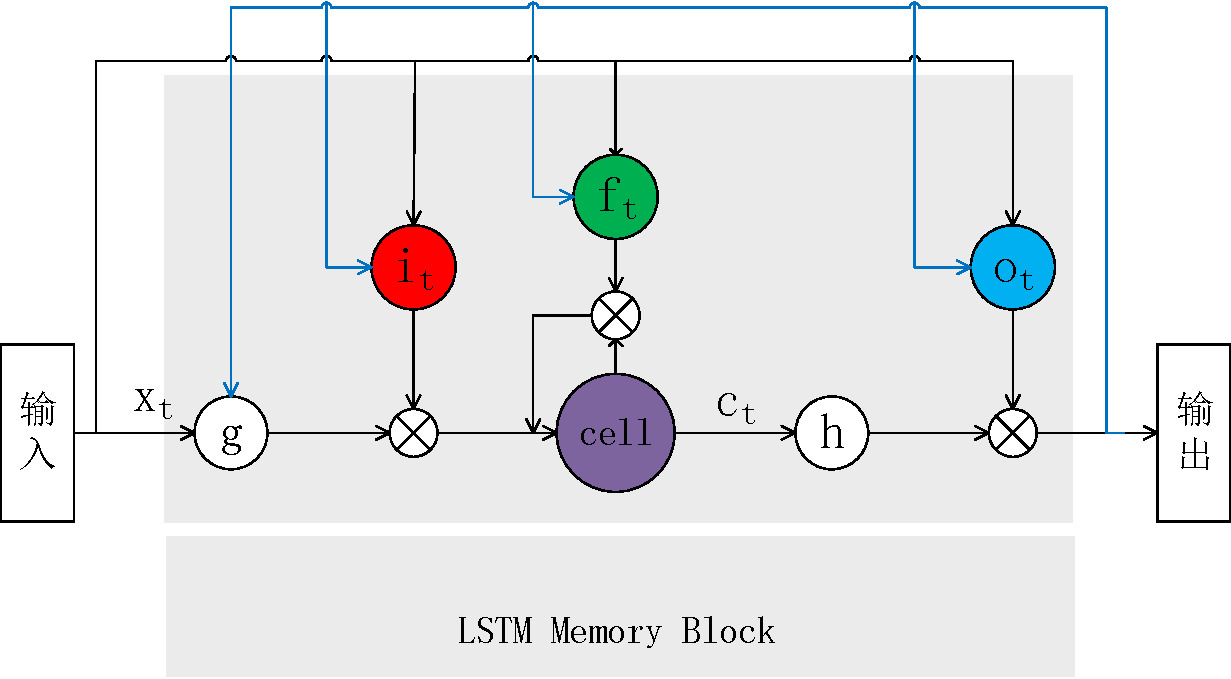
\includegraphics[width=1\textwidth]{figures/chapter3/lstm-crop}
\end{minipage}
}
\subfigure[LSTMP]{
\begin{minipage}[b]{0.45\textwidth}
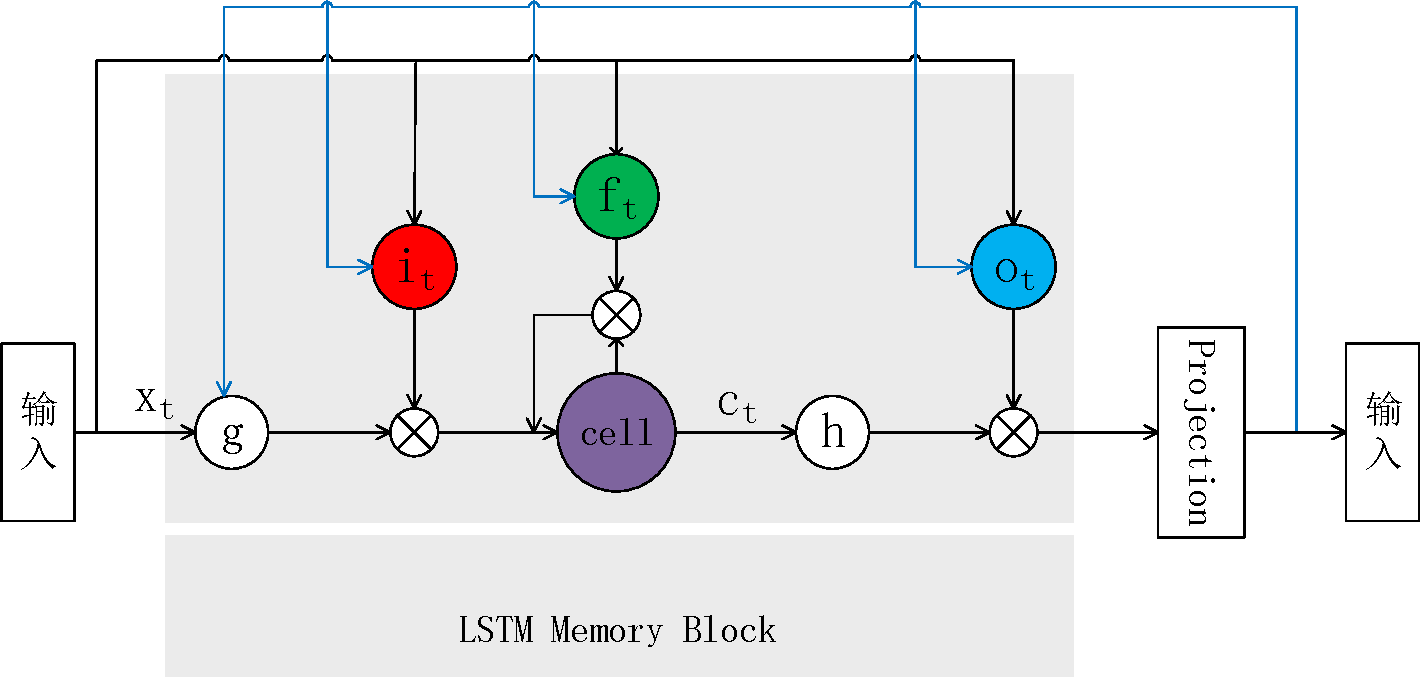
\includegraphics[width=1\textwidth]{figures/chapter3/lstmp-crop}
\end{minipage}
}
 \caption{LSTM的基本结构示意} \label{fig:lstm}
\end{figure}

标准的LSTM中,循环的连接直接从Memory Block的输出连接至Memory Block的输入和各个控制门。
2014年,Google首次将LSTM应用于大词汇量连续语音识别\ucite{sak2014long, sak2014long_lvsr},
Google研究人员将标准LSTM的输出连接到一个Projection层,然后将Projection的输出作为循环连接
到Memory Block的输入和控制门,这种结构成为LSTMP(LSTM with Projection),如图\ref{fig:lstm}
右图所示。在一般的设置中,LSTMP中的Projection层的节点数小于LSTMP中Memory Block的个数(比如Memory Block数量为1024,Projection可设为512),
这样有效减小了循环连接矩阵的大小。
通过Projection层,一方面减小了网络的参数数量,另一方面这种改进在声学模型上比标准LSTM取得更好的效果。
LSTMP的数据流向如下:
\begin{equation}
\label{equation:lstmp}
\begin{array}{l}
{{\rm{i}}_t} = \sigma ({W_{ix}}{x_t} + {W_{ih}}{h_{t - 1}}{\rm{ + }}{b_i})\\
{f_t} = \sigma ({W_{fx}}{x_t} + {W_{fh}}{h_{t - 1}}{\rm{ + }}{b_f})\\
{o_t} = \sigma ({W_{ox}}{x_t} + {W_{oh}}{h_{t - 1}}{\rm{ + }}{b_o})\\
{c_t} = {f_t} \odot {c_{t - 1}} + {i_t} \odot \tanh ({W_{cx}}{x_t} + {W_{ch}}{h_{t - 1}}{\rm{ + }}{b_c})\\
{{\rm{m}}_t} = {o_t} \odot \tanh ({c_t})\\
{h_t} = {W_m}{m_t}
\end{array}
\end{equation}
其中,$W_m$为Projection层的变换矩阵。由式\ref{equation:lstmp}可以看出,在LSTMP中Memory Block的输出$m_t$并不直接回连到自身,
而是先通过Projection层的$W_m$做矩阵变化后,再回连到Memory Block。

\section{混合神经网络}

目前,在大多数语音识别任务上,基于CNN和LSTM的声学模型均能取得比基于DNN的声学模型更好的效果。
那么一个很自然的想法就是,能否将三者结合使用,各取所长,相互补充。
CNN对频率各种变化具有较好的不变性,长于提取局部特性和特征;
LSTM有记忆功能,长于对时序序列建模;
DNN长于特征抽象和映射。
2015年,Google的工作\ucite{sainath2015convolutional}表明,通过三种网络结合的混合结构CLDNN(CNN+LSTM+DNN),
在大词汇量连续语音识别任务上,相比LSTM得到更低的语音识别错误率。

\subsection{CLDNN的基本结构}

Google提出的CLDNN的基本结构如图\ref{fig:cldnn}左图所示。
首先,为了对频率变化更好的建模,在网络底层使用1层或多层的卷积层CNN,使用卷积和池化操作;
网络中间是多层的LSTM结构,对CNN的输出进行时序建模;
LSTM层之后紧接多层的DNN,用于深化网络结构,提供更强大的建模能力。

\begin{figure}[htbp]
\centering
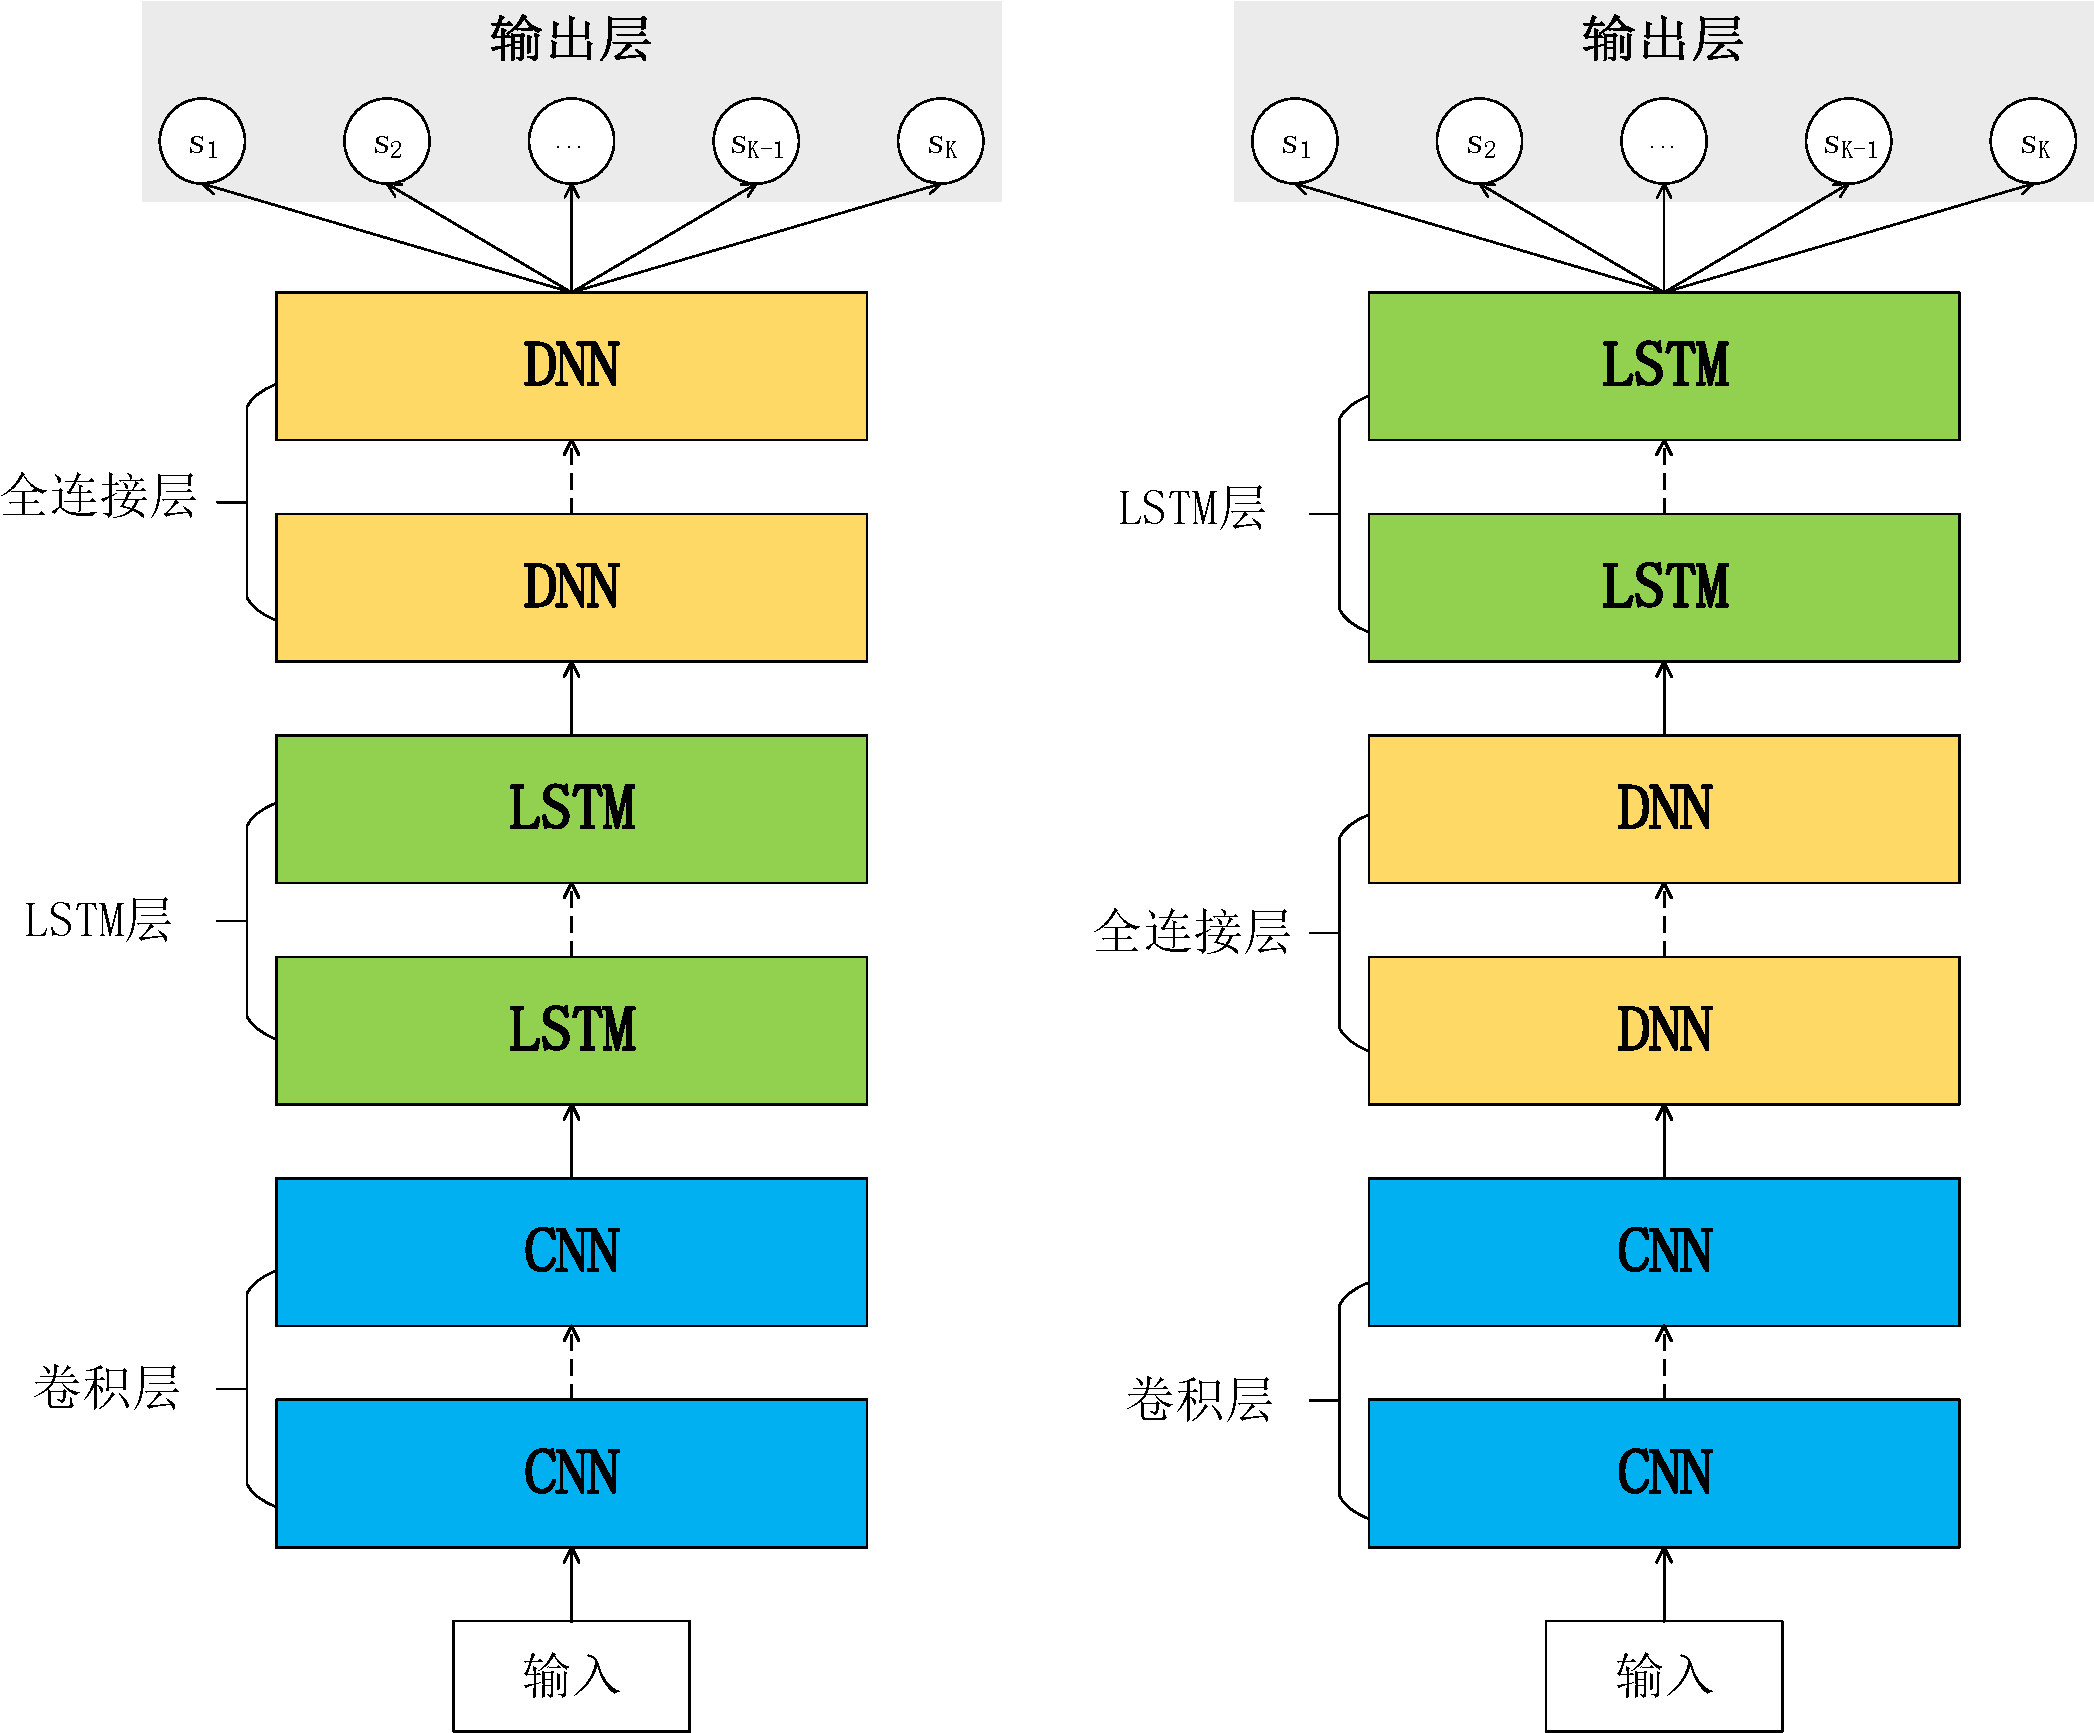
\includegraphics[width=0.8\textwidth]{figures/chapter3/cldnn-crop}
\caption{CLDNN的基本结构}
\label{fig:cldnn}
\end{figure}

在实际的应用过程中,我们发现可以做一些顺序上的调整。
声学模型的输入是频谱特征,所以长于频谱建模的CNN必须置于网络最下层。
但是DNN和LSTM层的位置是可调的,LSTM层也可以放在CNN和DNN之后,如图\ref{fig:cldnn}右图所示,
目前证明两种结构均能取得不错的效果。LSTM层放在CNN之后一个潜在的优点是相对DNN,
LSTM的梯度更不稳定,根据误差反向传播原理,深度神经网络梯度传递到低层时容易出现梯度爆炸或弥散的问题,
LSTM位置越靠近顶层,反馈回来的梯度稳定性能更好一点,从而整个网络的稳定性更好;
另一个潜在的优点是,基于已有DNN和CNN的识别网络(相当于已经预训练好的深层结构),
可以直接在其输出层之前插入多层的LSTM,快速得到CLDNN的结构训练并部署,
并与之前的系统进行比较。


\subsection{CLDNN跳帧训练}

基于DNN的声学模型在通用语音识别上的取得成功后,人们迫切的希望将其应用于手机等的嵌入式设备。
但DNN计算量庞大,在这些设备上往往是性能瓶颈,在实际应用时如何减小和优化DNN的计算量成为硬需。
跳帧训练最早在基于DNN\ucite{vanhoucke2013multiframe}的语音识别任务中提出,
当时在保证性能基本不下降的情况下,成倍的减小了计算量。

CNN、LSTM和CLDNN应用成功,使跳帧训练的应用更为广泛。
CNN的输入基于频谱特征,在输入层上需要依赖当前帧的左右上下文(Context),即需要特征拼帧输入,
这样在一帧的输入中,其实已经包含了左右几帧的特征信息。
LSTM的强大的序列建模能力,比DNN能够更好的进行跳帧时的平滑预测;
CLDNN结合了两者的优点,跳帧预测能力则更强。
一般语音训练的语料平均长度在4至6秒,语音识别特征以10ms为帧移,所以特征的帧率为100帧/秒,
且通过拼帧后,相邻帧之间还会有特征重叠。
近来的研究\ucite{sak2015fast, amodei2015deep, miao2016simplifying}表明,这样的高帧率和重叠实际上是有冗余的。

\begin{figure}[htbp]
\centering
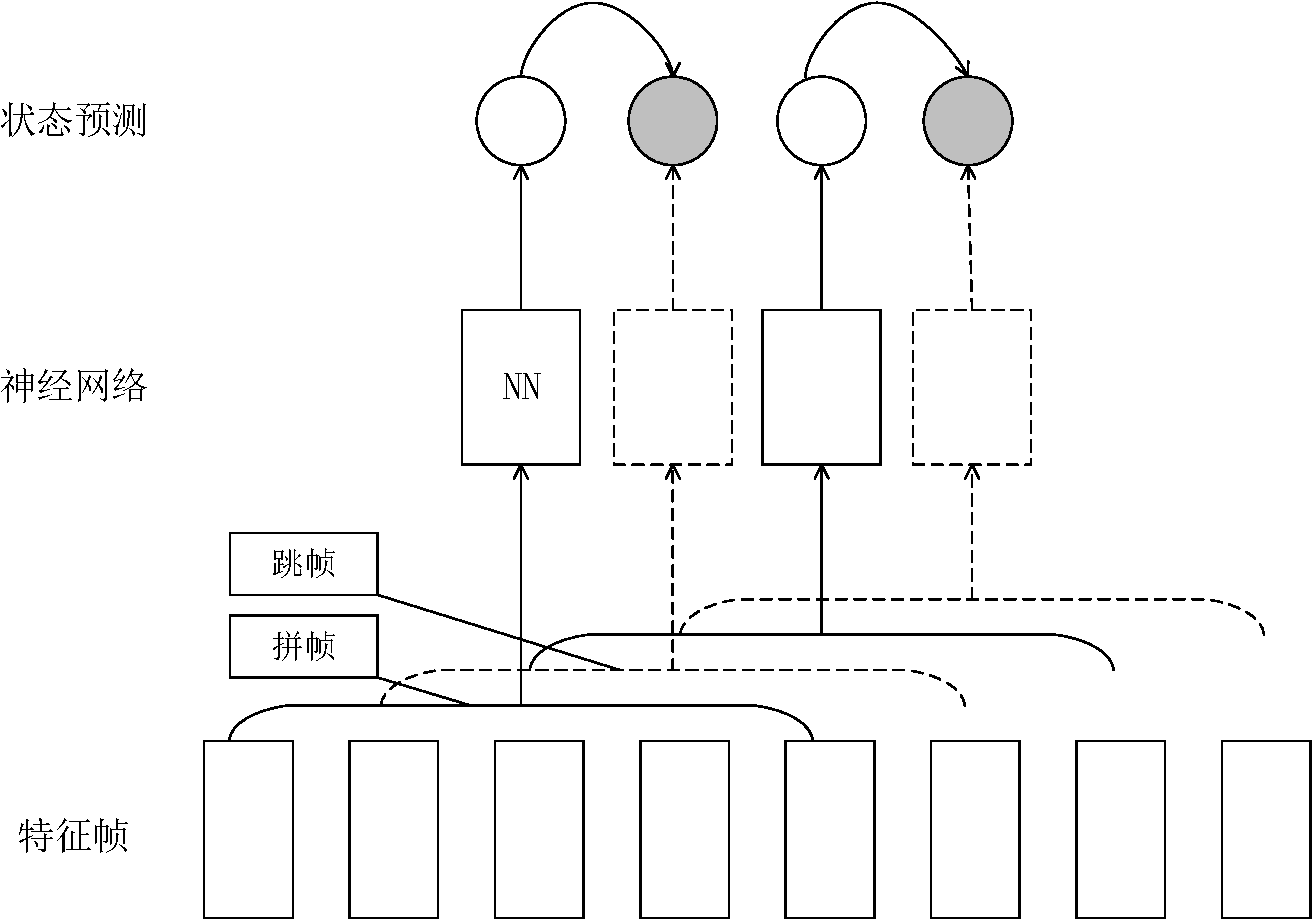
\includegraphics[width=0.5\textwidth]{figures/chapter3/skip-crop}
\caption{跳帧训练(跳1帧,虚线表示被跳过的训练数据)}
\label{fig:skip}
\end{figure}


跳帧训练的基本结构如图\ref{fig:skip}所示,网络输入层通过拼帧形成宽上下文,图中共拼5帧,每2帧跳1帧,
图中虚线表示被跳过的训练数据。跳帧训练时忽略被跳过的训练数据,所以能够有效成倍减小训练序列长度,
相当于对拼帧后的训练数据进行了降采样。
在识别预测时,有两种方法。
第一,仅使用选中帧(图中实线)进行预测,被跳过状态(图中灰色圈)的预测直接拷贝前一个选中帧的神经网络预测,称之为Copy模式;
第二,假设跳帧训练设置为N帧跳1帧,则将预测序列按按顺序分为N份$\{0, N, 2N, ...\}$, $\{1, N+1, 2N+1, ...\}$, ..., $\{N-1, 2N-1, 3N-1, ...\}$,
分别在网络中进行前向打分,最后将N份预测按顺序组织起来作为整体的预测,即$\{0, 1, ..., N, ..., 2N, ...\}$,称之为Split模式。


跳帧训练能有效的减小序列长度,提高训练速度,并加倍减少识别时神经网络的计算量。
在CTC的训练任务中,通过跳帧训练减小输入序列的长度,能有效提高CTC的训练的稳定性。

\section{Batch Normalization}

一般在准备深度神经网络的训练数据时,需要对训练数据进行归一化预处理。
最常用的的归一化操作使均值方差归一化MVN(Mean Variance Normalization),
即将训练数据通过减均值除以标准差的操作归一化到标准的正态分布。
通过归一化MVN操作,将输入映射到标准的高斯空间,利于训练的收敛性和模型效果。

2015年,Google的工作\ucite{ioffe2015batch}表明,同样可以在神经网络的中间层的输入上进行类似的MVN操作。
训练深度神经网络是个复杂多变的过程,神经网络中每一层的输入的分布都会随着训练逐渐改变,
这导致了神经网络的收敛速度慢,并且需要设置较小的学习率和更精细的初始化来保证神经网络的收敛性。
所以,类似输入层的归一化,可以通过归一化网络每一层的输入来解决该问题。

在训练中,对每一层的输入进行归一化时,由于计算全局的归一化代价很高,并且不可导,即不能使用梯度方法进行优化。
神经网络在训练过程中,使用mini-batch训练方法,mini-batch中含有多个训练样本。
基于mini-batch可以在归一化时,对归一化进行如下简化:
\begin{enumerate}
\item 使用mini-batch的归一化,即使用mini-batch的均值和方差替代全局的均值和方差。
\item 假设各维输入独立不相关,对每一层输入的每一维进行独立的归一化。
\end{enumerate}

假设mini-batch~${\rm B}$的大小为N,假设$x_k$表示${\rm B}$中任意一维输入的第$k$个样本,即
\begin{equation}
{\rm B}{\rm{ = }}\{ {x_1},{x_2},...,{x_N}\}
\end{equation}
计算每一维的均值和方差:
\begin{equation}
\begin{array}{l}
{\mu _{\rm B}} = \frac{1}{N}\sum\limits_{i = 1}^N {{x_i}} \\
\sigma _{\rm B}^2 = \frac{1}{N}\sum\limits_{i = 1}^N {({x_i} - } {\mu _{\rm B}}{)^2}
\end{array}
\end{equation}
则归一化的输出${\hat x}_i$可以表示为:
\begin{equation}
{{\hat x}_i} = \frac{{{x_i} - {\mu _{\rm B}}}}{{\sqrt {\sigma _{\rm B}^2 + \varepsilon } }}
\end{equation}
其中,$\varepsilon$是为防止除0引入的常量加项。

注意到仅仅使用这种简单的归一化可能会改变神经网络层的表征能力。
例如,tanh的输入通过这种简单归一化后,其激励会集中在坐标轴附近,
如图\ref{fig:activation},在坐标轴附近,tanh函数为近似的线性函数,
所以简单归一化必然降低了tanh的非线性映射能力。
为了解决该问题,使得变化满足镜像变换的能力,即从自身映射到自身,
对于每一维输入$x_i$引入一对参数$\gamma _i$和$\beta _i$,并且:
\begin{equation}
{y_i}{\rm{ = }}{\gamma _i}{{\hat x}_i} + {\beta _i}
\end{equation}
$y_i$是最终Batch Normalization的输出,当
${\gamma _i} = \sqrt {\sigma _{\rm B}^2 + \varepsilon }$
并且${\beta _i} = {\mu _{\rm B}}$时:
\begin{equation}
{y_i} = {x_i}
\end{equation}
即实现了镜像变换。$\gamma _i$和$\beta _i$是可以训练的参数,并且可导,
可以通过神经网络的优化同步训练。

在训练过程中,可以统计所有训练数据在神经网络每一层输入做前向时产生的均值和方差。
因此,在测试时,可以直接使用由训练数据统计的均值和方差。
假设训练过程中统计的任意一维输入$x_i$的全局均值为$E\left[ {{x_i}} \right]$,
全局方差为$Var[{x_i}]$,则在预测时:
\begin{equation}
\begin{array}{l}
{{\hat x}_i} = \frac{{{x_i} - E\left[ {{x_i}} \right]}}{{\sqrt {Var[{x_i}] + \varepsilon } }}\\
{y_i}{\rm{ = }}{\gamma _i}{{\hat x}_i} + {\beta _i}
\end{array}
\end{equation}

在深度神经网络中,对于普通的全连接层,Batch Normalization的位置在线性变换之后,激活函数之前,即:
\begin{equation}
y = f(BN(Wx + b))
\end{equation}
在卷积神经网络CNN中,对卷积后的每维输出均进行归一化,所以Batch Normalization的位置在卷积层和Max Pooling层
之间。对于LSTM,研究\ucite{laurent2015batch}表明,在多个位置做归一化并不有效,而仅对输入做Batch Normalization
证明有效。

众多的实验\ucite{ioffe2015batch, laurent2015batch, amodei2015deep}表明,使用Batch Normalization不仅可以设置更大的学习率,而且可以加快网络的收敛速度,
并进一步提高模型的效果。因此,在神经网络的训练过程中如若遇到收敛速度慢或者梯度问题导致无法
收敛时,可以尝试使用Batch Normalizaiton来解决。目前,Batch Normalization已作为深度神经网络
优化的标配之一。

\section{实验}

本节给出基于DNN、CNN、LSTM和CLDNN的声学建模实验,并在CLDNN基础上给出跳帧实验结果,并进行实验分析。

\subsection{数据和模型}

本实验使用的数据集为西北工业大学音频语音与语言处理研究组ASLP(Audio Speech and Language Processing, ASLP)标准数据集aslp128。
aslp128为中文普通话朗读数据,来自手机和桌面录音,共128小时,69689句,单句平均时长为6.61s,其中66205句作为训练,剩余3484句作为交叉验证集。
测试集使用西北工业大学音频语音与语言处理研究组标准测试集test3000,共3063句。

本实验使用语音识别工具Kaldi\ucite{povey2011kaldi},深度神经网络使用的对齐由aslp128数据集的GMM-HMM系统产生,共有CD-State状态5365个。
GMM-HMM系统使用39维的MFCC特征,所有深度神经网络均使用40维FBank(Filter Bank)特征。

实验中,使用5隐层的DNN,隐层节点为1024,使用特征为40维Fbank特征,左右各拼5帧以更好的利用上下文信息,所以输入特征共440维。

CNN中在网络输入层使用1层的CNN,上面叠加4层的DNN,DNN的隐层节点数同样为1024。CNN中同样使用40维Fbank特征,
不使用差分特征,左右各拼5帧,共440维输入特征。CNN中的卷积层的滤波器数量,滤波器的大小、步长和步移为可调参数;
Max Pooling层的Pooling的宽度和步移为可调参数。

LSTM可以自动学习到上下文信息,因此输入特征不使用拼帧,直接使用40维FBank特征。
由于LSTMP(图\ref{equation:lstmp})在语音识别任务中优于LSTM,本文中使用的LSTM均为LSTMP结构。
其中LSTMP的Cell为1024,Projection为512。

在CLDNN中,使用(CNN+DNN+LSTM)的结构,即CNN在网络最下层,DNN在中间,LSTM在上层的CLDNN结构。
所以,CLDNN中的输入特征配置与CNN相同,即40维FBank特征,左右各拼5帧,共440维输入特征。

本实验中,CNN、LSTM、CLDNN均存在多个可调参数,以下直接给出最优的参数配置。
CNN中卷积层使用128个滤波器,其中滤波器大小为$11 \times 9$,滤波器步移为1;
Max Pooling层的步长为4,步移为4,CNN的输出为1024维。
根据Google\ucite{sak2014long, sak2014long_lvsr}的工作,LSTM中使用2层的LSTMP,Cell为1024,Projection为512。
CLDNN使用1层的CNN,1层的DNN和2层的LSTM,其中CNN配置与CNN网络类似,DNN节点数位1024,
LSTM同样使用Cell1024,Projection512。

实验中,CNN和DNN所用激活函数为Simoid激活函数。相邻层之间,使用Batch Normalization做输入的归一化。

\subsection{帧识别率分析}

基于交叉熵CE的声学模型训练中,评价声学模型性能的一个重要指标是帧识别率Frame Accuracy,即对单帧的语音特征进行状态分类的正确率。
一般来说,帧识别率越高,单帧语音特征分类正确率越高,最终语音识别率也会越准确。
当然,最终的语音识别率是声学模型、语言模型、解码算法共同作用的结果。
图\ref{fig:acc}给在aslp128数据集的训练过程中,DNN、CNN、LSTM和CLDNN在交叉验证集(Cross Validition)的帧识别率。

\begin{figure}[htbp]
\centering
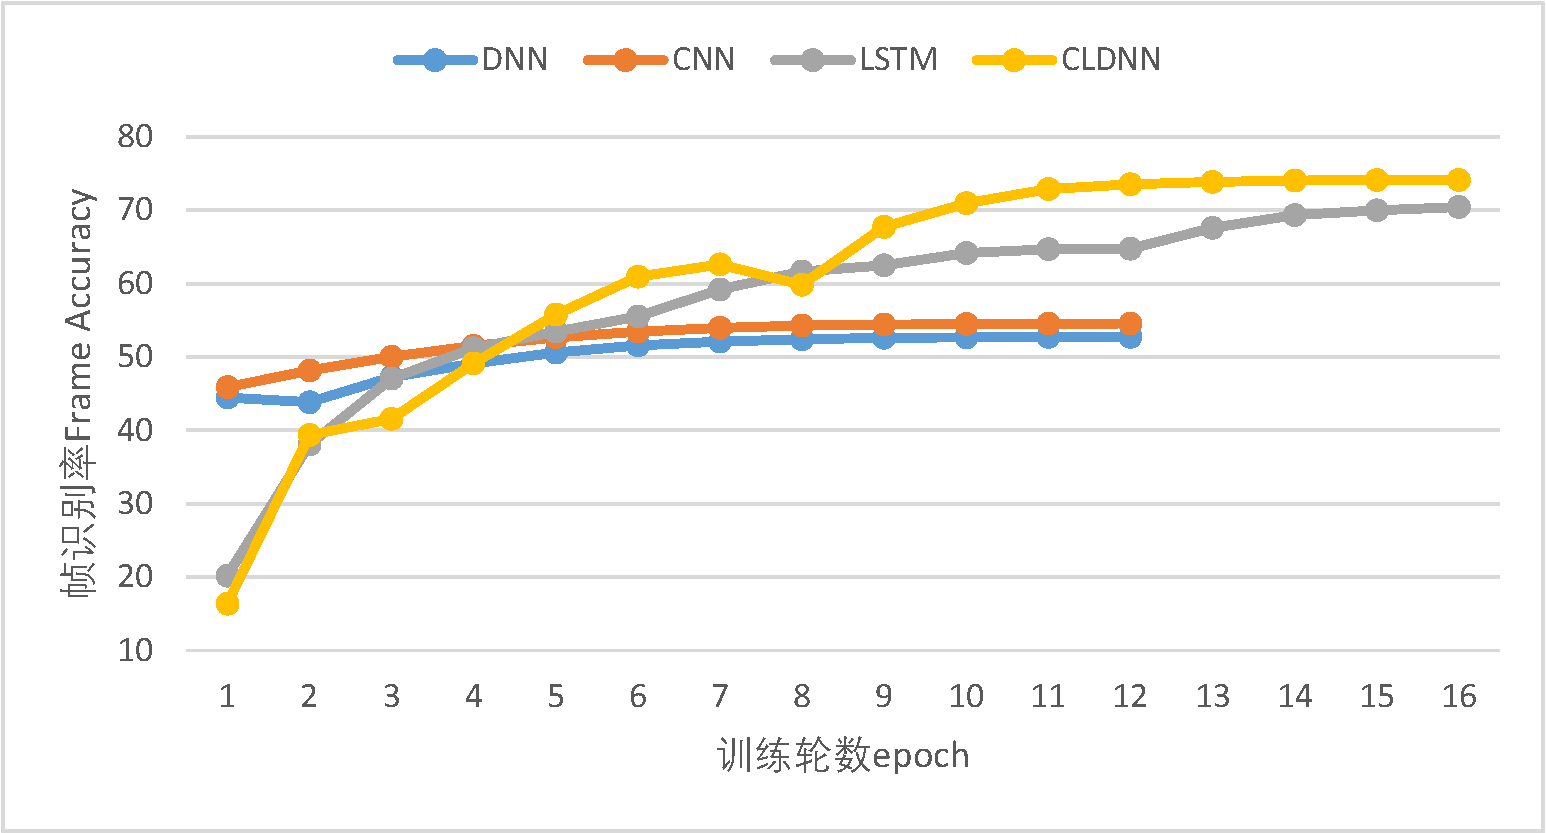
\includegraphics[width=0.8\textwidth]{figures/chapter3/acc-crop}
\caption{aslp128数据集DNN、CNN、LSTM和CLDNN训练中的帧识别率}
\label{fig:acc}
\end{figure}

由图\ref{fig:acc}可以看出,在训练中,CNN的帧识别率略好于DNN。
在LSTM中,得益于其出色的时间序列建模能力,LSTM的帧识别率远远高于DNN和CNN,LSTM的帧识别率相对于DNN提升近20个百分点。
CLDNN结合了CNN、DNN和LSTM的优点,帧识别率比LSTM的效果更好。

\subsection{实验结果与分析}

表\ref{table:aslp128-cldnn}给出aslp128数据集上DNN、CNN、LSTM和CLDNN识别结果,
其中CER为中文语音识别字错误率(Character Error Rate),CER列中括号内的数值表示错误率相对DNN的下降百分比。
参数量为该深度神经网络所含参数量,以M(百万)为单位。

\begin{table}[htbp]
\centering
\caption{aslp128数据集DNN、CNN、LSTM和CLDNN识别结果}
\fontsize{10.5pt}{10.5pt}\song \vspace{0.5em}
%\begin{tabularx}{\textwidth}{*4{>{\centering\arraybackslash}X}@{}}
\begin{tabularx}{\textwidth}{cYcc}
\toprule
编号 & 模型结构         & 参数量(M) & CER  \\ \midrule
1  & DNN(5DNN)              & 9.12   & 11.25         \\
2  & CNN(1CNN\_4DNN)    & 8.68   & 10.81(3.39\%) \\
3  & LSTM(2LSTMP)         & 10.27  & 11.05(1.78\%) \\
4  & 2DNN+2LSTM   & 12.78  & 10.63(5.51\%) \\
\textbf{5}  & \textbf{CLDNN(1CNN\_1DNN\_2LSTMP)} & \textbf{12.75}  & \textbf{10.23(9.07\%)} \\ \bottomrule
\end{tabularx}
\label{table:aslp128-cldnn}
\end{table}

由表\ref{table:aslp128-cldnn}可以看出,在aslp128数据集上,CNN相对基线系统DNN提升3.39\%;
直接使用2层LSTM在该数据集上作用不明显,分析可能是网络仅有2层、参数也有限导致,
因此在2层LSTM基础上结合DNN使用,同时增加了网络的深度和参数量,CER获得明显提升;
CLDNN在该数据集上取得最好效果,相对基线系统提升9.07\%。

\subsection{跳帧}

在CLDNN基础上,进一步在aslp128数据集上研究跳帧对CLDNN的影响。
在该实验中,使用\ref{table:aslp128-cldnn}中CLDNN的基本配置,即1CNN\_1DNN\_2LSTMP的网络结构,参数量为12.75M。
解码时分别使用Copy和Split模式解码,
通过设置不同的跳帧宽度,得到表\ref{table:aslp128-skip}实验结果。

\begin{table}[htbp]
\centering
\caption{aslp128 CLDNN跳帧实验}
\fontsize{10.5pt}{10.5pt}\song \vspace{0.5em}
\begin{tabularx}{\textwidth}{YYYY}
\toprule
编号 & Skip Width & CER(Copy) & CER(Split)     \\ \midrule
1  & no skip    & \multicolumn{2}{c}{10.23}  \\
2  & skip 2     & 10.32     & \textbf{10.13} \\
3  & skip 3     & 11.08     & 10.56          \\
4  & skip 4     & 11.79     & 11.05          \\ \bottomrule
\end{tabularx}
\label{table:aslp128-skip}
\end{table}

通过分析表\ref{table:aslp128-skip}可以得出以下结论,
\begin{enumerate}
\item 跳帧训练通过合适的配置在同一数据集上能达到与不跳帧相当的模型精度,甚至可能更好的模型效果,
    例如表中通过2帧跳1帧的训练方式和Split解码,最终识别结果优于不跳帧的CLDNN。
\item 通过比较解码模式,解码使用Split模式要优于简单的Copy模式。
\end{enumerate}
如前文所述,使用Skip能减少句子序列长度,有效提高训练速度和训练稳定性。
此外,Copy模式的解码可以有效的成倍减少解码时神经网络的计算量。

\subsection{更大的数据量}

更进一步,我们在更大的数据集上进行CLDNN的实验,进一步验证CLDNN和跳帧的效果。
本节实验使用地平线机器人科技hr400朗读数据集,训练集共400小时,测试集为9000句。
并且在该数据集训练中,CLDNN直接使用跳帧训练,跳帧宽度为3,以提高训练速度。
实验中模型配置我们在模型结构中注明,实验结果如表\ref{table:hr400-cldnn}

\begin{table}[htbp]
\centering
\caption{hr400数据集DNN、CNN、LSTM和CLDNN(跳帧)识别结果}
\fontsize{10.5pt}{10.5pt}\song \vspace{0.5em}
\begin{tabularx}{\textwidth}{cYcc}
\toprule
编号         & 模型结构                                                       & 参数量(M)           & CER                     \\ \midrule
1          & 5DNN(hidden1024)                                           & 5.43          & 18.31                   \\
2          & CNN(1CNN\_4DNN\_128filter)                                 & 4.12          & 17.27(5.68\%)           \\
3          & 2LSTM(Cell760\_Projection380)                              & 5.49          & 14.52(20.69\%)          \\
\textbf{4} & \textbf{CLDNN(1CNN\_1DNN\_2LSTMP\_Cell700\_Projection350)} & \textbf{5.81} & \textbf{14.12(22.88\%)} \\ \bottomrule
\end{tabularx}
\label{table:hr400-cldnn}
\end{table}

比较aslp128数据集上的结果,
在hr400数据集中,网络改进所带来的收益更大。
2层LSTM单独使用就能取得20.69\%的CER的收益,这与公开的LSTM声学模型的收益相当。
通过跳帧后的CLDNN更取得了22.88\%的收益,跳帧的效果进一步得到验证。

尽管两个数据集带来的收益大小不同,但我们看到,通过CLDNN,通过适应数据集的模型调试和参数调试,最终均能得到稳定的收益。

% !Mode:: "TeX:UTF-8"

\chapter{基于CD-Phone和CTC的语音识别}

无论是经典的HMM-GMM识别系统,还是基于HMM-DL的识别系统,均属于HMM的识别框架。
RNN的强大的时序序列建模能力在一定程度上可以学习HMM框架中的状态变化和跳转,
因此识别任务中RNN的引入,逐步淡化了HMM框架的作用。
HMM框架经过几十年的发展,已经非常的完善,
并且庞杂,深度学习引入识别任务后,
识别系统的结构进一步复杂,进行识别任务所需的步骤流程也越来越长。

因此,如何打破HMM框架,简化识别系统的流程,
进一步挖掘深度学习在语音识别任务上的能力成为目前语音识别研究的新热点之一\ucite{hannun2014deep, amodei2015deep, miao2015eesen}。
基于CD-Phone和CTC的语音识别是这些研究中的代表。
Phone和CD-Phone建模打破了经典的基于HMM状态CD-State建模的方法;
CTC的end-to-end的建模能力可以使基于深度学习的语音识别系统无需依赖经典的HMM-GMM框架,可以大幅度简化现有识别系统的流程。

本章分别介绍基于CD-Phone和CTC的语音识别,及其在声学建模中的应用。

\section{CD-Phone}

\subsection{传统建模单元CD-State} \label{seg:cdstate}

状态是HMM的基本建模单元,基于HMM的语音识别系统中每个音素Phone一般使用3状态的HMM。
在一般的语音识别系统中,音素的个数一般为几十个至上百个,例如TIMIT中音素数目为48,
汉语的语料库中即使带调的音素也不超过200。所以建模的单元数量少,建模不够精细。
为了对音素进行精确建模,可以进一步考虑音素所处的上下文,一般考虑音素所处位置的
前一个音素和后一个音素。例如对于音素b,我们可以建立a-b+c的三音素模型,其中a表示b
左边的音素,c表示b右边的音素。假设共有$N$个音素,考虑所有的上下文,一共可以得到$N^3$个三音素,
这样就解决了建模单元不够多,建模不够精细的问题。

然而,这样引进了新的问题。第一,建模单元太多,在训练数据固定的情况下,每个建模单元得到的训练数据不够充分;
第二,有一些三音素可能未在训练数据中出现,例如在汉语语料中,一般不会出现连续三个辅音的三音素,例如b-b+b,
z-z+z等。

\subsubsection{状态绑定Tied-State}

在经典的语音识别系统中,使用决策树和状态绑定(Tied-State)来解决这个问题。
状态绑定是指对于一个单音素的任意一个状态,该状态的一些三音素可以共享一个概率密度分布,即共享一个状态号,
例如a-b+a,e-b+a,i-b+a,o-b+a可以共享一个状态,因为他们的左上文\{a, e, i, o\}均为元音,
很可能在发音上具有相近性。通过状态绑定,一些发音相近的三音素状态可以共享相同的训练数据,
训练数据中未出现的三音素状态也可以绑定到已经出现的三音素上状态上,
这样即解决了训练数据稀疏和未出现三音素状态的建模问题。
最终,将决策树和状态绑定形成的三音素状态称为CD-State(Context Dependent State),以表明基本的聚类单元是状态,
并且状态是上下文相关的。

\begin{figure}[htbp]
\centering
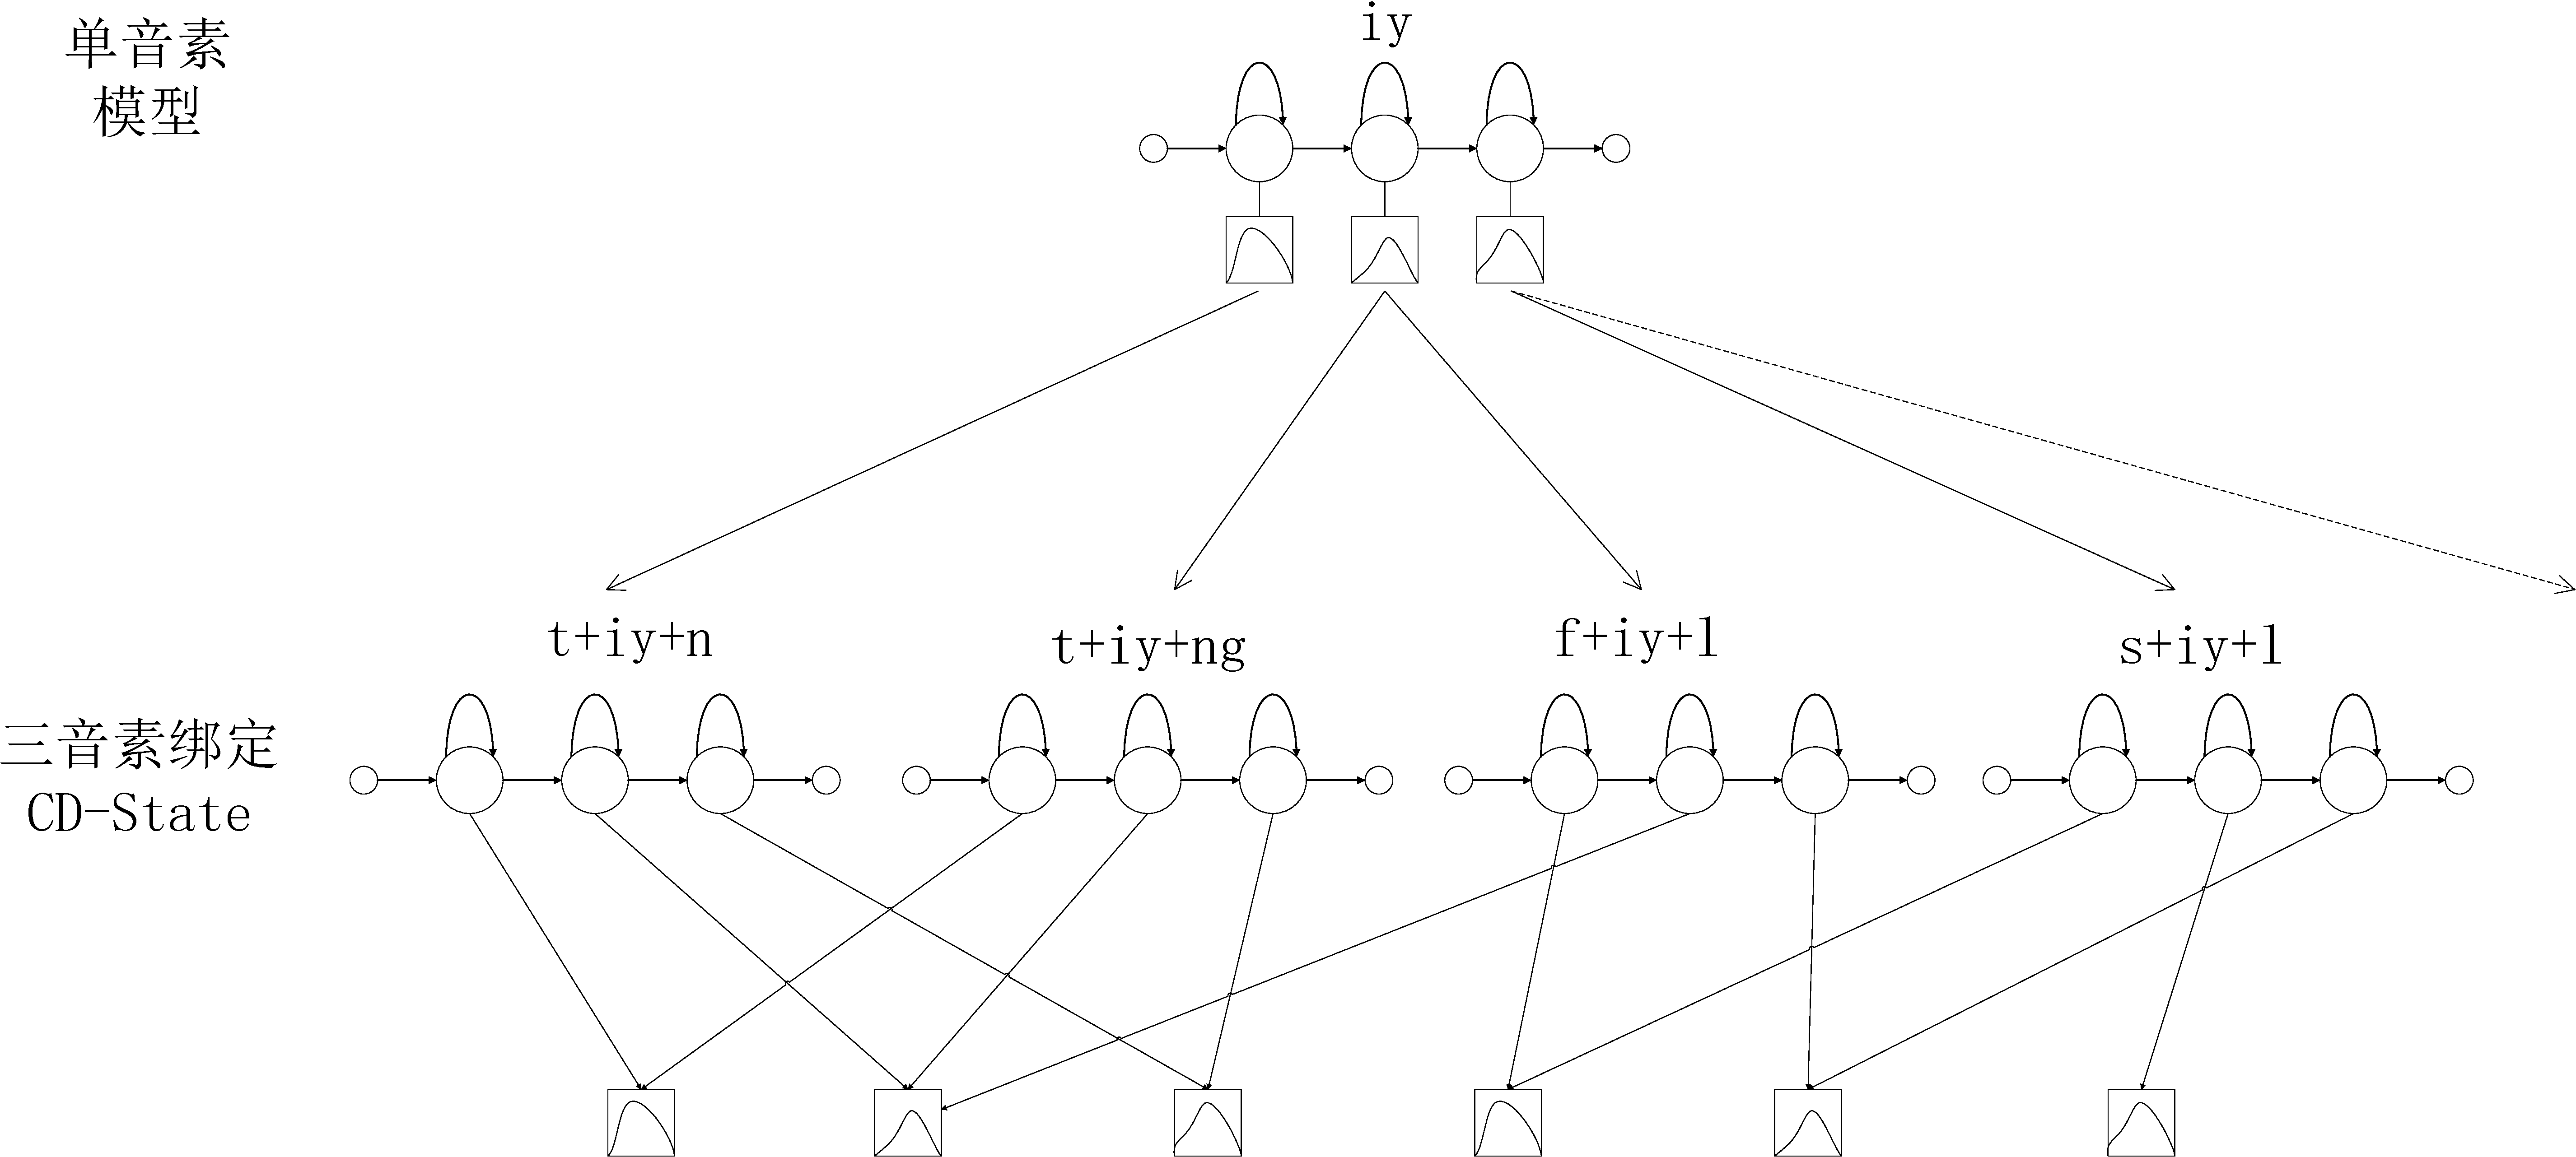
\includegraphics[width=1.0\textwidth]{figures/chapter4/cdstate-crop}
\caption{CD-State构建过程}
\label{fig:cdstate}
\end{figure}

HMM系统中CD-Stae的建立过程如图\ref{fig:cdstate}所示:
    \begin{enumerate}
        \item 首先建立和训练三状态的单音素的HMM模型。
        \item 使用已有单音素或三音素的模型得到三音素对齐,通过决策树建立状态绑定的三音素模型,迭代训练该模型。
        \item 重复2,直至模型训练充分。
    \end{enumerate}

\subsubsection{决策树}

上文提到建立CD-State的基本方法是决策树聚类。决策树是一个二叉树,在每个节点上都有相应的问题。
该问题相当于一个位置信息和一个音素集合,表示在当前层次,这个集合中的音素发音具有相近性。
对于三音素a-b+c,决策树会首先查看该节点的位置信息,通过位置信息确定是要判断b左边的音素还是右边的音素,
确定之后,然后判断该音素是否在该节点的音素集合中,若找到,
则走该节点的左子树,反之则走右子树。决策树的叶子节点表示最终三音素状态绑定的结果,
即该节点上的三音素共享相同的状态号。
对于任意一个三音素的给定HMM状态,通过该决策树就能查找到其最终的聚类结果。

\begin{figure}[htbp]
\centering
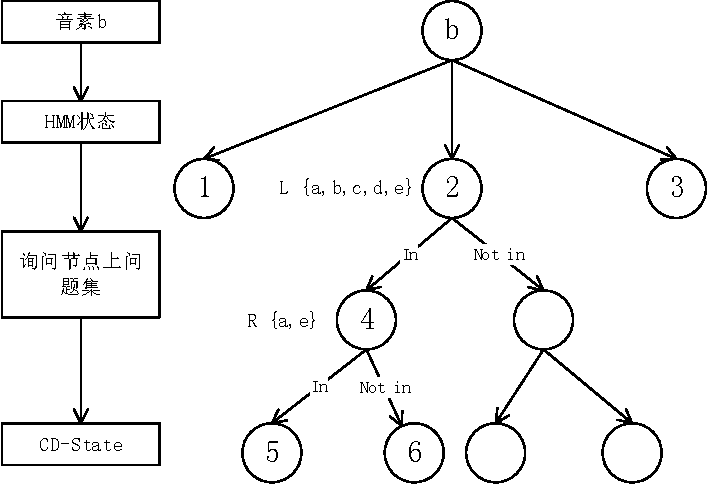
\includegraphics[width=0.6\textwidth]{figures/chapter4/tree-crop}
\caption{决策树示例}
\label{fig:tree}
\end{figure}

一个决策树的示例如图\ref{fig:tree}所示。根节点表示单音素,第二层表示单音素的三个状态,
第三层及其一下表示决策树状态决策过程。例如,对于三音素a-b+c的第二个状态,首先查找到状态2;
状态2上会看b的左边的音素是否在集合\{a, b, c, d, e\}中,判断为是,走到状态4;
接着判断a+b-c的右边状态是否在集合\{a, e\}中,判断为否,转到状态6;
状态6已经是叶子节点,查找结束。6即是三音素a-b+c的第二个HMM状态的聚类结果。

那么该决策树又是如何构建的呢?决策树是一个自上而下逐步构建的过程\ucite{young1994tree}。
首先,在单音素HMM状态的根节点上,所有的状态都被假设归位一类,然后计算其似然;
假设训练数据集为$S = ({x_1},...,{x_M}) \in ({R^N})$,其中$M$表示特征样本总数,$N$表示特征维度,
且各维特征相互独立(HMM-GMM系统中使用MFCC特征,使用对角高斯描述),则对于特征$\textbf{x}$,其似然为:
\begin{equation}
[P(x) = \frac{1}{{\prod\nolimits_{k = 1}^N {{{(2\pi \sigma _k^2)}^{1/2}}} }}\prod\limits_{k = 1}^N {\exp ( - \frac{1}{2}} \frac{{{{({x_k} - {\mu _k})}^2}}}{{\sigma _k^2}})
\end{equation}
对于集合$S$,其log似然为:
\begin{equation}
\begin{array}{l}
L(S) =  - \frac{1}{2}\sum\limits_{i = 1}^M {\left[ {\sum\limits_{k = 1}^N {\log (2\pi \sigma _k^2)}  + \sum\limits_{k = 1}^N {\frac{{{{({x_{ik}} - {\mu _k})}^2}}}{{\sigma _k^2}}} } \right]} \\
{\kern 1pt} {\kern 1pt} {\kern 1pt} {\kern 1pt} {\kern 1pt} {\kern 1pt} {\kern 1pt} {\kern 1pt} {\kern 1pt} {\kern 1pt} {\kern 1pt} {\kern 1pt} {\kern 1pt} {\kern 1pt} {\kern 1pt} {\kern 1pt} {\kern 1pt} {\kern 1pt} {\kern 1pt} {\kern 1pt} {\kern 1pt} {\kern 1pt} {\kern 1pt} {\kern 1pt} {\kern 1pt} {\kern 1pt}  =  - \frac{1}{2}\left[ {M\sum\limits_{k = 1}^N {\log (2\pi \sigma _k^2) + M} \sum\limits_{k = 1}^N {\frac{{\sigma _k^2}}{{\sigma _k^2}}} } \right]\\
{\kern 1pt} {\kern 1pt} {\kern 1pt} {\kern 1pt} {\kern 1pt} {\kern 1pt} {\kern 1pt} {\kern 1pt} {\kern 1pt} {\kern 1pt} {\kern 1pt} {\kern 1pt} {\kern 1pt} {\kern 1pt} {\kern 1pt} {\kern 1pt} {\kern 1pt} {\kern 1pt} {\kern 1pt} {\kern 1pt} {\kern 1pt} {\kern 1pt} {\kern 1pt} {\kern 1pt} {\kern 1pt}  =  - \frac{1}{2}\left[ {MN(1 + \log (2\pi ) + M\sum\limits_{k = 1}^N {\log (\sigma _k^2)} } \right]
\end{array}
\end{equation}
其中$\mu _k$表示集合$S$第$k$维的均值,$\sigma _k^2$表示集合$S$第$k$维的方差。
然后通过问题集中的一个问题将该节点分为两部分$S_l$和$S_r$,分别计算这两部分的似然和;
\begin{equation}
L({S_l}) + L({S_r}) =  - \frac{1}{2}\left[ {MN(1 + \log (2\pi ) + {M_l}\sum\limits_{k = 1}^N {\log (\sigma _{lk}^2) + {M_r}\sum\limits_{k = 1}^N {\log (\sigma _{rk}^2)} } } \right]
\end{equation}
遍历所有的问题集,选出似然增益和最大的问题作为最优问题;
\begin{equation}
\begin{array}{l}
{q^*} = \mathop {\arg \min }\limits_q L({S_{lq}}) + L({S_{rq}}) - L(S)\\
{\kern 1pt} {\kern 1pt} {\kern 1pt} {\kern 1pt} {\kern 1pt} {\kern 1pt} {\kern 1pt} {\kern 1pt} {\kern 1pt} {\kern 1pt} {\kern 1pt} {\kern 1pt} {\kern 1pt}  = \mathop {\arg \min }\limits_q \left[ {{M_l}\sum\limits_{k = 1}^N {\log (\sigma _{lk}^2) + {M_r}\sum\limits_{k = 1}^N {\log (\sigma _{rk}^2)} } } \right]
\end{array}
\end{equation}
其中$q^*$表示最优问题,并将根节点分为两部分。
然后递归的对所有分裂出来的新节点执行上述算法,
终止条件一般为,第一,每个节点上的在训练数据中的统计量已在小于设定临界值(避免该状态没有得到充分的训练数据);
第二,似然增益已小于设定阈值(该状态上所有绑定的三音素已足够相近); 两个条件满足其一即可。

\subsubsection{问题集}

在构建决策树时需要使用问题集,一个问题由一组声学上相近的音素组成,多个问题形成的集合即为问题集。
问题集的构建有两种方式:
\begin{enumerate}
\item 人工设计,根据语音和语言学的知识进行设计,与特定语言和任务相关,例如HTK\ucite{young2002htk}中即使用这种问题集。
\item 自动生成问题集,根据训练数据中的单音素对齐得到各个音素的发音特征,然后进行树聚类得到问题集。
\end{enumerate}
Kaldi\ucite{povey2011kaldi}中既可以使用人工设计的问题集,同时也能自动生成问题集,也可以两者结合使用。

\subsection{Phone和CD-Phone建模单元}

HMM建模的一个前提假设是状态的独立假设。在GMM和DNN中,当前时刻的状态预测仅与当前时刻的输出特征相关,
而在RNN中,因为RNN的内部状态,当前时刻预测输出不仅与当前时刻相关,而且还依赖历史时刻的输入。
所以,这一前提假设已经不成立,而且RNN强大的时序建模能力已经能够拟合HMM所描述的状态变化和跳转过程。
所以,直接使用Phone进行建模,使用RNN表述Phone的变化过程成为一种新思路。

使用Phone作为建模单元的过程如下:
\begin{enumerate}
\item 通过HMM-GMM系统得到状态对齐,进一步得到Phone对齐;
\item 直接Phone对齐训练基于Phone的RNN的声学模型。
\end{enumerate}
在解码时,HMM中的三状态约束使一个Phone至少持续三帧数据,基于Phone的解码时也要类似限制Phone的最小持续时间,
来保证解码出来的Phone的具有明确的时长持续变化,如图\ref{fig:duration}所示。

\begin{figure}[htbp]
\centering
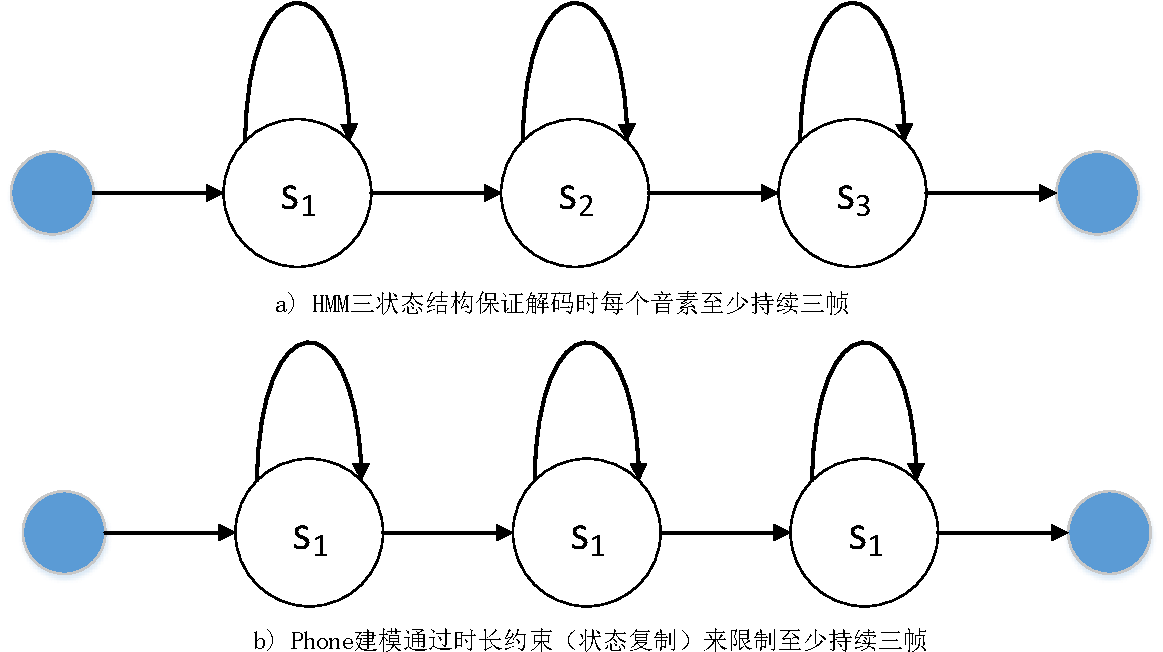
\includegraphics[width=0.6\textwidth]{figures/chapter4/duration-crop}
\caption{基于Phone的解码}
\label{fig:duration}
\end{figure}

在中文中,音节Syllable是发音的基本单元,中文汉字发音为声韵母的组合。
因此在中文数据集中,可以使用Syllable作为基本建模单元。

但是,直接使用Mono Phone建模存在着与Mono Phone HMM状态建模相似的问题,即建模单元太少,建模不够精细。
使用与CD-State相似的概念,我们使用CD-Phone(Context Dependent Phone),给Phone加入上下文,
再通过聚类来结解决该问题。

CD-State聚类时,直接使用帧级状态对齐特征进行聚类。然而,Phone是一个有内部变化的建模单元,
在做聚类时需要考虑Phone的变化过程。Google在其CD-Phone\ucite{senior2015context}的工作中提出,
使用HMM-GMM系统中Phone的三个状态来描述Phone特征,使用三状态对齐的中值(均值)作为该Phone的特征,
如图\ref{fig:3middle}使用三状态的中值来表示Phone的聚类特征。

\begin{figure}[htbp]
\centering
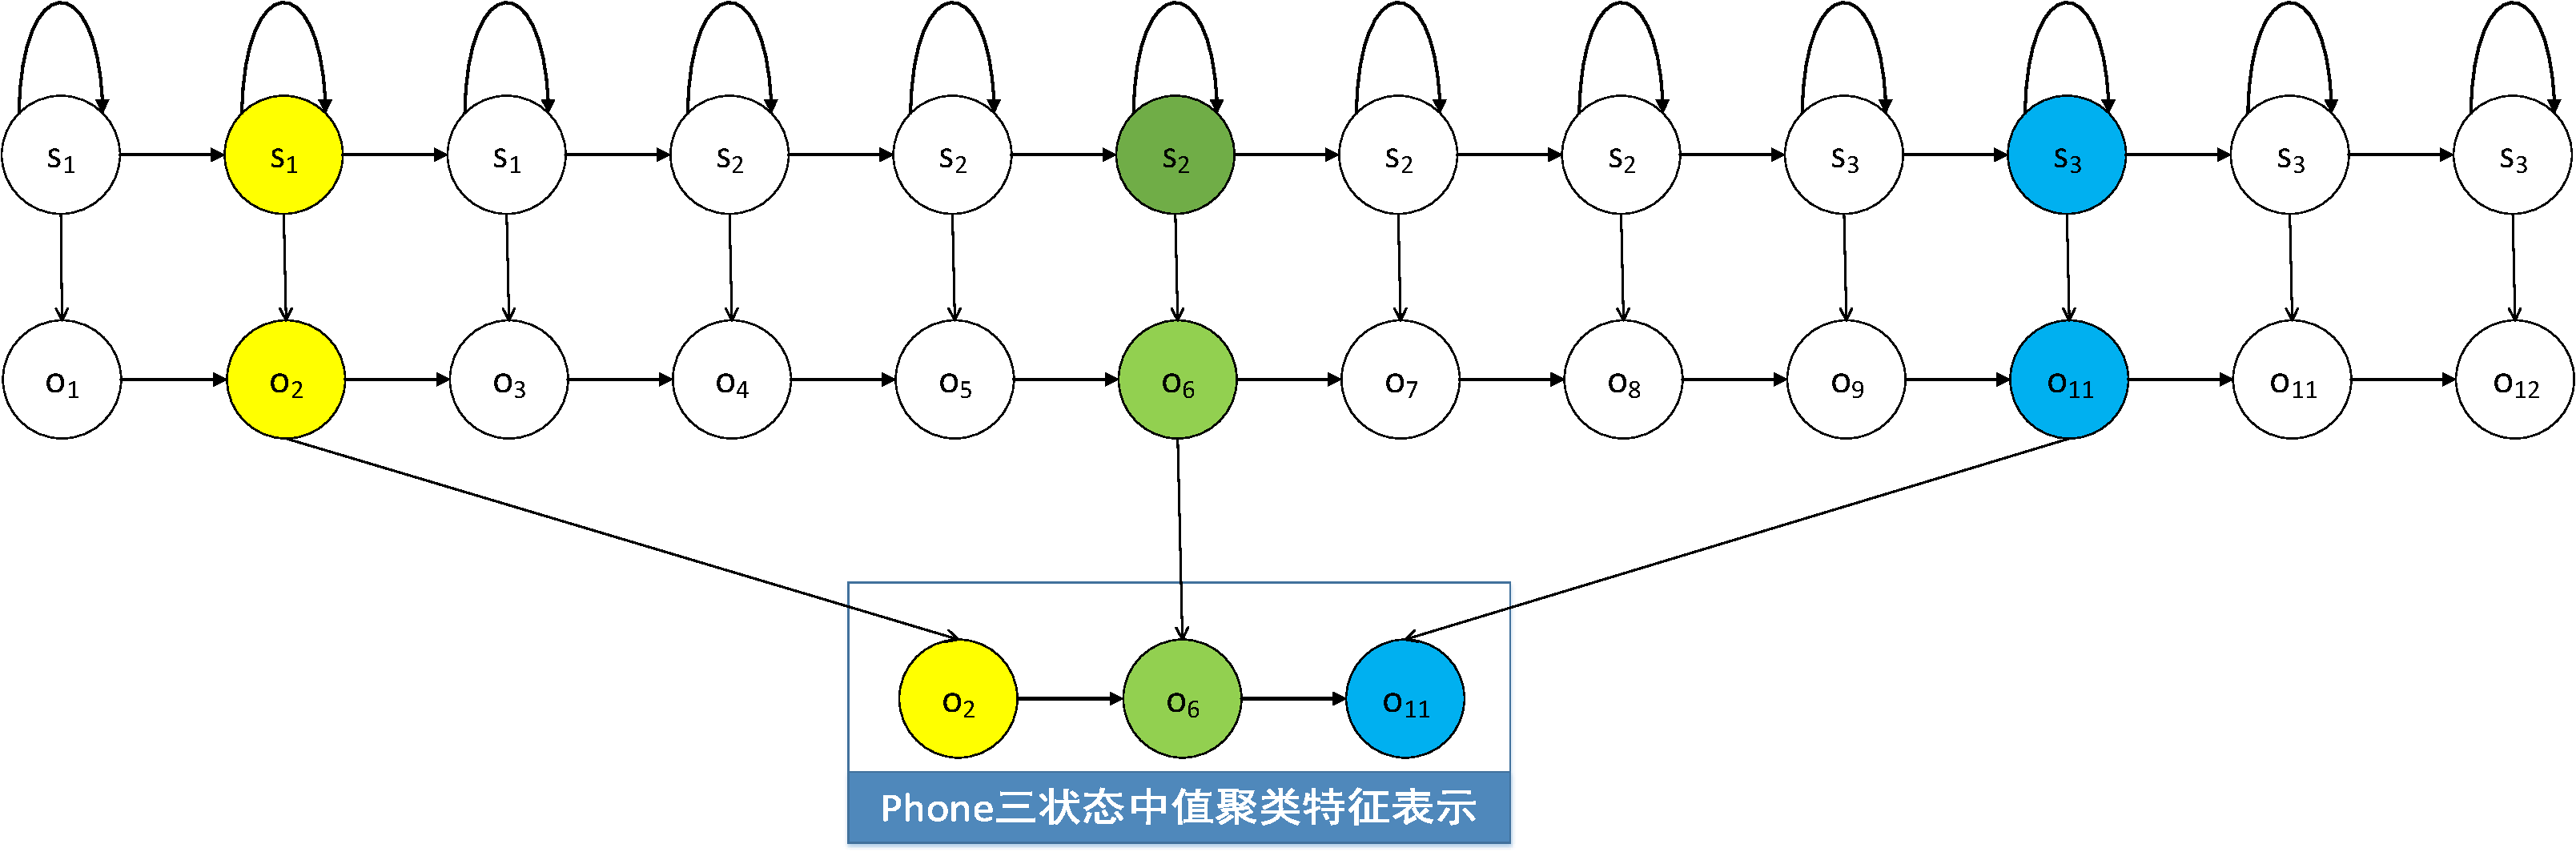
\includegraphics[width=0.8\textwidth]{figures/chapter4/3middle-crop}
\caption{CD-Phone聚类中Phone的特征表示}
\label{fig:3middle}
\end{figure}


使用CD-Phone作为建模单元的过程如下,
\begin{enumerate}
\item 通过HMM-GMM系统得到三音素状态CD-State对齐;
\item 按如上方法进行Phone特征统计,然后使用\ref{fig:cdstate}节类似方法使用问题集和决策树方法进行聚类;
\item 将CD-State对齐转换为CD-Phone的对齐;
\item 使用CD-Phone对齐训练基于RNN的CD-Phone的声学模型。
\end{enumerate}
在解码时,与Phone的解码类似,同样需要约束CD-Phone的最小持续时长。


\section{CTC}

如前文所述,基于深度神经网络的语音识别系统需要依赖HMM-GMM系统生成的状态对齐,复杂化了语音识别系统的流程。
语音识别本质上也是个序列标注任务,HMM方法是解决序列标注任务的一种经典方法之一。
CTC(Connectionist Temporal Classificatio)\ucite{graves2006connectionist, graves2012neural},
于2006年由Alex Graves提出,则是解决序列标注任务的另一种经典方法。

\subsection{基本概念}

在序列标注任务中,假设字符表的大小为$L$,CTC的softmax层输出则共有$L+1$个单元。
在给定输入的情况下,其中后$L$个用于预测当前时刻分别处在这$L$个字符上的概率;
另外一个为辅助单元,称之为blank(空白),用于预测在当前时刻不产生任何输出的概率,即空白。
所以,CTC在同一时刻的输出,可以使字母表中的任意一个字符,也可以是blank。

假设训练集为$S$,给定输入序列$\textbf{x}$,其长度为$T$,其对应字符标注序列记为$textbf{l}$,
$y_k^t$表示在$t$时刻观测到字符$k$的概率,其中$k<=L$; $k=0$表示输出blank单元的概率。
则序列$\textbf{x}$的任意一个等价序列$\pi$出现的概率可以表示为:
\begin{equation}
\label{euqation:ctcpath}
{\rm{p}}(\pi |\bf{x},S) = \prod\limits_{t = 1}^T {{\rm{y}}_{{\pi _t}}^t}
\end{equation}
其中$\pi  \in {L^{'T}}$,$L^{'T}$表示在输入序列$\textbf{x}$的标注中任意位置插入任意长度的blank,直至其总长度为$T$。
在后面介绍中,省略训练数据$S$,将$\rm{p}(\pi |\bf{x},S)$简记为$\rm{p}(\pi|\bf{x})$。

定义映射函数{\rm B},表示将CTC的预测序列经过消除连续出现的字符和去除blank之后的序列。
例如${\rm B}(a - ab - ) = {\rm B}( - aa -  - abb) = abb$。
直观上看,当从连续的字符到一个新字符,或者由blank到一个非blank字符时,即认为是新的字符。
我们称之为序列等价性。这个性质使CTC可以使用未分段的数据,因为该性质无需预先知道字符出现的时刻。
这里可以看出blank的另一个作用,即允许预测序列出现两个连续相同的字符,只要这两个字符之间存在blank即可。

根据序列等价性,$\bf{l}$的条件概率可以表示为:
\begin{equation}
\label{euqation:ctcallpath}
p({\bf{l}}|{\bf{x}}) = \sum\limits_{\pi  \in {{\rm B}^{ - 1}}({\bf{l}})}^{} {p(\pi |{\bf{x}})}
\end{equation}

理论上,CTC可以使用任意结构的RNN,但为了对当前字符做更精准的预测,一般使用双向的RNN,
这样可以有效的利用前向和后向所有历史信息。

\subsection{前向后向算法}

在给出$p({\bf{l}}|{\bf{x}})$ 的形式之后,
我们可以使用与HMM的前向后向算法\ref{section:probability}类似的动态规划思想来计算$p({\bf{l}}|{\bf{x}})$的概率。
即该问题具有最优子结构,可以通过迭代填表的方式求得。

首先,定义${{\bf{l'}}}$表示在$\bf{l}$的开始,结束和相邻两个字符之间插入blank后的序列,则${{\bf{l'}}}$的长度为$2|{\bf{l}}| + 1$。
在计算过程中,我们允许从当前一个字符直接跳到下一个字符;或者从当前字符跳到自身;或者从当前字符跳到blank。

定义${\alpha _{\rm{t}}}(s)$表示$t$时刻到达第$s$个字符的前向概率和,则
\begin{equation}
{\alpha _{\rm{t}}}(s) = P({\pi _{1:t}}:B({\pi _{1:t}}) = {{\bf{l}}_{1:s/2}},{\pi _t} = {{l'}_s}{\rm{|}}{\bf{x}}{\rm{) = }}\sum\limits_{\scriptstyle{\kern 1pt} {\kern 1pt} {\kern 1pt} {\kern 1pt} {\kern 1pt} {\kern 1pt} {\kern 1pt} {\kern 1pt} {\kern 1pt} {\kern 1pt} {\kern 1pt} {\kern 1pt} {\kern 1pt} {\kern 1pt} \pi :\hfill\atop
\scriptstyle\beta ({\pi _{1:t}}) = {{\bf{l}}_{1:s/2}}\hfill} {\prod\limits_{t' = 1}^t {y_{{\pi _{t'}}}^{t'}} }
\end{equation}
$s/2$表示去掉blank的标注。

由以上定义,标注序列$\bf{l}$的概率可以表示为$t$时刻处在最后一个字符或者其后blank上的概率和,表明允许以最终字符或者blank结束:
\begin{equation}
p({\bf{l}}|{\bf{x}}) = {\alpha _T}(|{\bf{l'}}|) + {\alpha _T}(|{\bf{l'}}| - 1)
\end{equation}
同理,允许序列可以以第一个字符或者blank起始,则可以得到${\alpha _{\rm{t}}}(s)$的初始值:
\begin{equation}
\begin{array}{l}
{\alpha _1}(1) = y_b^1\\
{\alpha _1}(2) = y_{{l_1}}^1\\
{\alpha _1}(s) = 0,\forall s > 2
\end{array}
\end{equation}
${\alpha _{\rm{t}}}(s)$可以由${\alpha _{\rm{t-1}}}(s)$,${\alpha _{\rm{t-1}}}(s-1)$,${\alpha _{\rm{t-1}}}(s-2)$递推计算:
\begin{equation}
\label{equation:alpha}
{\alpha _{\rm{t}}}(s) = y_{{{l'}_s}}^t\left\{ \begin{array}{l}
\sum\nolimits_{i = s - 1}^s {{\alpha _{{\rm{t - 1}}}}(i){\kern 1pt} ;} {\kern 1pt} {\kern 1pt} {\kern 1pt} {\kern 1pt} {\kern 1pt} {\kern 1pt} {\kern 1pt} {\kern 1pt} {\kern 1pt} {\kern 1pt} {\kern 1pt} {\kern 1pt} {\kern 1pt} {{l'}_s} = b{\kern 1pt} {\kern 1pt} {\rm{or}}{\kern 1pt} {\kern 1pt} {{l'}_{s - 2}} = {{l'}_s}\\
\sum\nolimits_{i = s - 2}^s {{\alpha _{{\rm{t - 1}}}}(i){\kern 1pt} ;} {\kern 1pt} {\kern 1pt} {\kern 1pt} {\kern 1pt} {\kern 1pt} {\kern 1pt} {\kern 1pt} {\kern 1pt} {\kern 1pt} {\kern 1pt} {\kern 1pt} {\kern 1pt} {\rm{otherwise}}
\end{array} \right\}
\end{equation}
CTC前向跳转的一个示意如图\ref{fig:ctcforback}所示,图中给出DOG的CTC状态跳转图。
其中空心圈表示blank,实心圈表示字符,横向为时间轴,纵向为字符轴。
从左上角到右下角即为一个可能的路径。


\begin{figure}[htbp]
\centering
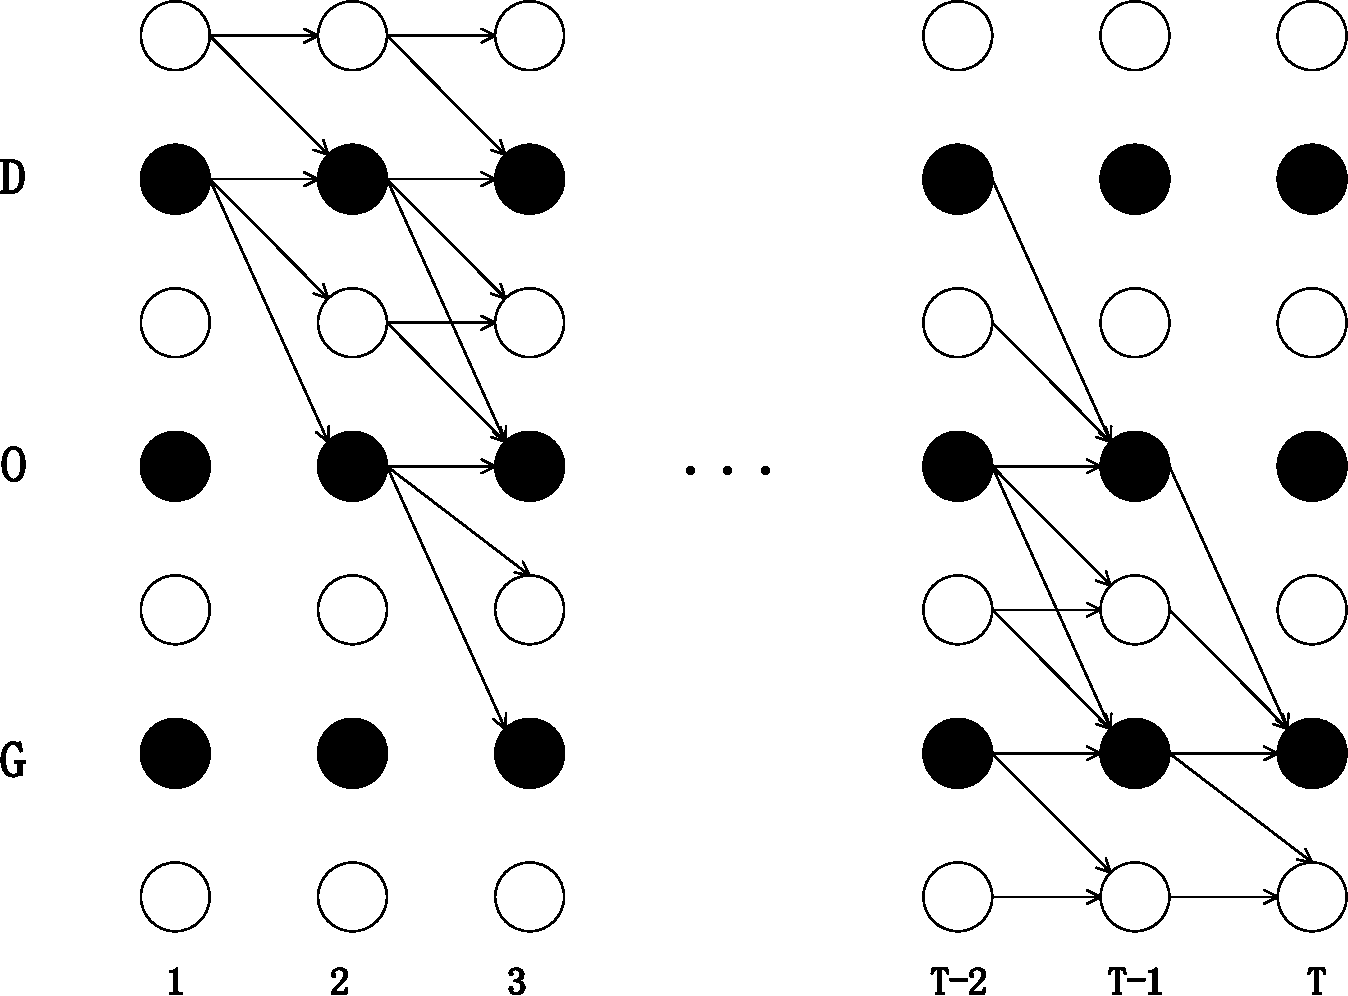
\includegraphics[width=0.6\textwidth]{figures/chapter4/forback-crop}
\caption{CTC前向状态跳转}
\label{fig:ctcforback}
\end{figure}

定义${\beta _{\rm{t}}}(s)$表示$t$时刻到达第$s$个字符的后向概率和,则
\begin{equation}
{\beta _{\rm{t}}}(s) = P({\pi _{{\rm{t}} + 1:T}}:B({\pi _{t:T}}) = {{\bf{l}}_{s/2:{\rm{|}}{\bf{l}}|}},{\pi _t} = {{l'}_s}{\rm{|}}{\bf{x}}{\rm{) = }}\sum\limits_{\scriptstyle{\kern 1pt} {\kern 1pt} {\kern 1pt} {\kern 1pt} {\kern 1pt} {\kern 1pt} {\kern 1pt} {\kern 1pt} {\kern 1pt} {\kern 1pt} {\kern 1pt} {\kern 1pt} {\kern 1pt} {\kern 1pt} \pi :\hfill\atop
\scriptstyle\beta ({\pi _{t:T}}) = {{\bf{l}}_{s/2:{\rm{|}}{\bf{l}}|}}\hfill} {\prod\limits_{t' = t + 1}^T {y_{{\pi _{t'}}}^{t'}} }
\end{equation}
同理,允许序列可以以最后一个字符或者其后的blank结束,则可以得到${\beta _{\rm{t}}}(s)$的初始值:
\begin{equation}
\begin{array}{l}
{\beta _T}(|{\bf{l'}}|) = 1\\
{\beta _T}(|{\bf{l'}}| - 1) = 1\\
{\beta _T}(s) = 0,\forall s < |{\bf{l'}}| - 1
\end{array}
\end{equation}
${\beta _{\rm{t}}}(s)$的递推计算公式为:
\begin{equation}
\label{equation:beta}
{\beta _{\rm{t}}}(s) = y_{{{l'}_s}}^t\left\{ \begin{array}{l}
\sum\nolimits_{i = s}^{s + 1} {{\beta _{{\rm{t + 1}}}}(i){\kern 1pt} y_{{{l'}_s}}^{t + 1};} {\kern 1pt} {\kern 1pt} {\kern 1pt} {\kern 1pt} {\kern 1pt} {\kern 1pt} {\kern 1pt} {\kern 1pt} {\kern 1pt} {\kern 1pt} {\kern 1pt} {\kern 1pt} {\kern 1pt} {{l'}_s} = b{\kern 1pt} {\kern 1pt} {\rm{or}}{\kern 1pt} {\kern 1pt} {{l'}_{s + 2}} = {{l'}_s}\\
\sum\nolimits_{i = s}^{s + 2} {{\beta _{{\rm{t + 1}}}}(i){\kern 1pt} y_{{{l'}_s}}^{t + 1};} {\kern 1pt} {\kern 1pt} {\kern 1pt} {\kern 1pt} {\kern 1pt} {\kern 1pt} {\kern 1pt} {\kern 1pt} {\kern 1pt} {\kern 1pt} {\kern 1pt} {\kern 1pt} {\rm{otherwise}}
\end{array} \right\}
\end{equation}


实际应用中,由于计算机字长限制,上述概率的连乘运算会很快下溢。
所以该概率计算一般转到$log$域,上述递推公式\ref{equation:alpha}~\ref{equation:beta}中也存在加法,
$log$域中加法的一个有用等式是:
\begin{equation}
\ln (a + b) = \ln (a + \ln (1 + {e^{\ln b - \ln a}}))
\end{equation}
这样即解决了前向后向算法中的数值问题。

\subsection{CTC目标函数}

如上文所述,CTC的目标函数由最大似然的方法得到。并且,CTC的目标函数可导,
因此可以通过梯度的方法对CTC进行优化。
CTC的下层网络结构为RNN,同样可以通过梯度方法优化。
因此CTC在计算得到梯度后,通过反向传播的方法回传给网络,
进一步进行基于CTC损失函数的RNN网络的优化。

定义目标函数$O$表示整个训练集的负log域的概率和,则$O$可以表示为:
\begin{equation}
{\rm{O}} =  - \ln (\prod\limits_{({\bf{x}},{\bf{z}}) \in S} {p({\bf{z}}|{\bf{x}})} ) =  - \sum\limits_{({\bf{x}},{\bf{z}}) \in S}^{} {\ln p({\bf{z}}|{\bf{x}})}
\end{equation}
首先,计算$O$对网络输出的梯度:
\begin{equation}
\label{equation:o}
\frac{{\partial O}}{{\partial y_k^t}} =  - \frac{{\partial \ln p({\bf{z}}|{\bf{x}})}}{{\partial y_k^t}} =  - \frac{1}{{p({\bf{z}}|{\bf{x}})}}\frac{{\partial p({\bf{z}}|{\bf{x}})}}{{\partial y_k^t}}
\end{equation}
使用前向后向算法有:
\begin{equation}
{\alpha _{\rm{t}}}(s){\beta _{\rm{t}}}(s) = \sum\limits_{\scriptstyle\pi  \in {{\rm B}^{ - 1}}({\bf{z}})\hfill\atop
\scriptstyle{\kern 1pt} {\kern 1pt} {\kern 1pt} {\kern 1pt} {\pi _t} = {{z'}_s}\hfill} {\prod\limits_{t = 1}^T {y_{{\pi _t}}^t} }
\end{equation}
由\ref{euqation:ctcpath}有:
\begin{equation}
{\alpha _{\rm{t}}}(s){\beta _{\rm{t}}}(s) = \sum\limits_{\scriptstyle\pi  \in {{\rm B}^{ - 1}}({\bf{z}})\hfill\atop
\scriptstyle{\kern 1pt} {\kern 1pt} {\kern 1pt} {\kern 1pt} {\pi _t} = {{z'}_s}\hfill} {p(} \pi |{\bf{x}})
\end{equation}
由\ref{euqation:ctcallpath},通过全概率公式(在$t$时刻可以输出${\bf{z}}$序列中的任意字符),所以:
\begin{equation}
\label{equation:alls}
p({\bf{z}}|{\bf{x}}) = \sum\limits_{s = 1}^{|{\bf{z'}}|} {{\alpha _{\rm{t}}}(s){\beta _{\rm{t}}}(s)}
\end{equation}

为了计算对$y_k^t$的梯度,需要考虑在$t$时刻通过字符$k$的所有路径。
由于相同的字符或者blank可以在一个序列中出现多次,
因此定义$lab({\bf{z}},k) = \{ s:{{z'}_s}{\rm{ = k\} }}$表示序列$\bf{z}$中出现字符$k$的集合:
\begin{equation}
\frac{{\partial {\alpha _{\rm{t}}}(s){\beta _{\rm{t}}}(s)}}{{\partial y_k^t}} = \left\{ \begin{array}{l}
\frac{{{\alpha _{\rm{t}}}(s){\beta _{\rm{t}}}(s)}}{{y_k^t}},if{\kern 1pt} k{\kern 1pt} {\kern 1pt} in{\kern 1pt} {\kern 1pt} {\bf{z'}}\\
0,{\kern 1pt} {\kern 1pt} {\kern 1pt} otherwise
\end{array} \right\}
\end{equation}
对\ref{equation:alls}求导得:
\begin{equation}
\frac{{\partial p({\bf{z}}|{\bf{x}})}}{{\partial y_k^t}} = \frac{1}{{y_k^t}}\sum\limits_{s \in lab({\bf{z}},k)}^{} {{\alpha _{\rm{t}}}(s){\beta _{\rm{t}}}(s)}
\end{equation}
代入\ref{equation:o}得:
\begin{equation}
\label{equation:ctcloss}
\frac{{\partial O}}{{\partial y_k^t}} =  - \frac{1}{{p({\bf{z}}|{\bf{x}})y_k^t}}\sum\limits_{s \in lab({\bf{z}},k)}^{} {{\alpha _{\rm{t}}}(s){\beta _{\rm{t}}}(s)}
\end{equation}
最后,计算对输出层$a_k^t$的梯度,$a_k^t$为softmax函数之前$t$时刻第$k$个字符单元的激励,
\begin{equation}
\label{equation:alldiff}
\frac{{\partial O}}{{\partial a_k^t}} = \sum\limits_{k'} {\frac{{\partial O}}{{\partial y_{k'}^t}}} \frac{{\partial y_{k'}^t}}{{\partial a_k^t}}
\end{equation}
根据softmax\ref{equation:softmax}函数,有
\begin{equation}
\label{equation:softmaxdiff}
\frac{{\partial y_{k'}^t}}{{\partial a_k^t}} = y_{k'}^t({\delta _{kk'}} - y_k^t)
\end{equation}
将\ref{equation:ctcloss}和\ref{equation:softmaxdiff}代入\label{equation:alldiff}得:
\begin{equation}
\frac{{\partial O}}{{\partial a_k^t}} = y_k^t - \frac{1}{{p({\bf{z}}|{\bf{x}})}}\sum\limits_{s \in lab({\bf{z}},k)}^{} {{\alpha _{\rm{t}}}(s){\beta _{\rm{t}}}(s)}
\end{equation}

\subsection{CTC的特性}

经过上面的讨论,可以总结出CTC的三点特性:
\begin{enumerate}
\item blank,CTC在建模中引入辅助建模单元blank,表示不作任何输出;
\item 序列等价性,连续的相同的字符可以归约为单个字符,归约后blank被消除;
\item 尖峰(Peak)预测特性,这是CTC在预测时的现象,其在大多数时刻上输出为blank,并且预测时输出呈尖峰状,如图\ref{fig:peak}。
\end{enumerate}

\begin{figure}
\centering
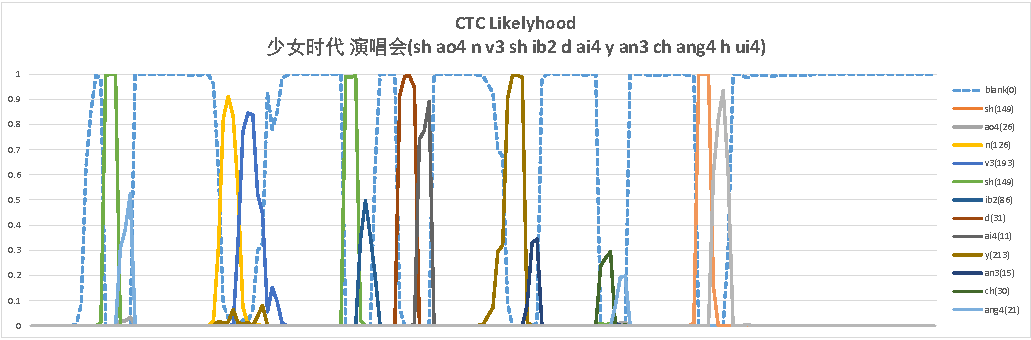
\includegraphics[width=1.0\textwidth]{figures/chapter4/peak-crop}
\caption{CTC Peak预测}
\label{fig:peak}
\end{figure}

\subsection{语音识别中的应用}

语音识别任务是个天然的序列标注任务,因此可以使用CTC预测声学模型中的建模单元。
Alex Graves在2008年已经将CTC应用在TIMIT的音素识别任务上\ucite{graves2012neural}。
2015年,Miao的EESEN\ucite{miao2015eesen}在WSJ数据集上应用CTC。
同年,Google\ucite{sak2015fast}和百度\ucite{amodei2015deep}也均成功将CTC应用在大词汇量连续语音识别任务中。

在这些任务中,建模单元各有不同。
EESEN中使用Phone或者Character作为建模单元,
Google的工作中使用Phone或CD-Phone作为作为建模单元,
百度的Deep Speech 2系统在中文中使用字,英文中使用Character作为建模单元。
本文主要研究使用Phone和CD-Phone作为建模单元的CTC。

在传统的HMM语音系统中,一般使用基于WFST\ucite{mohri2004weighted}的解码器。
基于WSFT的解码器中,将HMM(H),上下文(C,Context)、词典(L,Lexicon)、语言模型(G,Grammar)通过
WFST的组合(Compose)操作构成解码图HCLG\ucite{mohri2002weighted},然后在HCLG的WFST图上进行语音识别的解码算法。

在基于CTC的语音识别中,已经摒弃了HMM,因此需要重新构图。
将CTC的基本单元构图记为T,则T的结构如图\ref{fig:t}所示:
\begin{figure}[htbp]
\centering
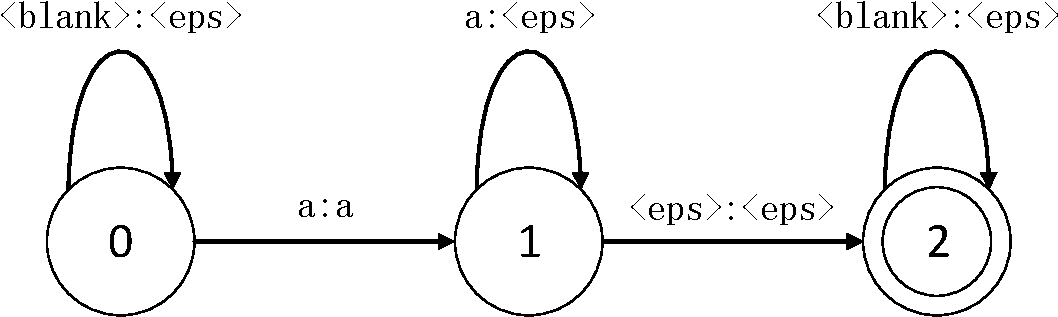
\includegraphics[width=0.5\textwidth]{figures/chapter4/t-crop}
\caption{CTC基本单元的WFST图}
\label{fig:t}
\end{figure}
由图中的跳转可以看出,解码时在一个CTC的基本单元内,
起始状态0可以经过任意个个blank;
从状态0输入a并输出a到达状态1,状态1上可以输入任意个a,输出为空;
状态1也可以经过空跳转<eps>到达状态2;
状态2为终结点,类似状态1,可以输入任意个blank。
通过该WFST,即可以保证CTC的一个建模单元中,前后均可以有任意个blank,
中间有任意个单元a,并且整个单元的输出为1个a,满足序列等价归约的性质。

在得到T的结构后,与HCLG类似。我们可以使用WFST的组合操作使T和更高层次的
上下文C(可选),词典L和语言模型G进行组合。
假设T中含上下文,则最终解码图WFST图S可以表示为:
\begin{equation}
{\rm{S = T}} \circ {\rm{min(det(L}} \circ {\rm{G))}}
\end{equation}
若不含上下文,S可以表示为:
\begin{equation}
{\rm{S = T}} \circ {\rm{min(det(C}} \circ {\rm{L}} \circ {\rm{G))}}
\end{equation}
其中det表示WFST的确定化操作,min表示WFST的最小化操作。

近来,Google、百度的研究\ucite{senior2015context, sak2015fast, sak2015learning, hannun2014deep, amodei2015deep}表明,
CTC不仅可以进一步提升声学建模的精度;
并且由于CTC尖峰预测的特性,CTC在主路径上的打分很强,可以远远超过竞争路径。
语音识别的解码中一般使用Beam Search\ucite{young1989token}的方法进行剪枝,
在同样的beam阈值条件下,相对于交叉熵CE的模型,
CTC解码中的竞争路径会被更快的裁剪,因此基于CTC的语音识别解码具有非常快的解码速度。
这对大幅度提升语音识别系统的响应速度和提供线上系统的吞吐量均具有重要意义。

\section{实验}

本节介绍基于Phone、CD-Phone和Syllable的声学建模实验,
并给出在这三种建模单元基础上结合CTC在中文语音识别任务上的实验结果。

\subsection{数据和模型}

以Phone、Syllable和CD-Phone为建模单元的声学模型和CTC都依赖于大量的数据。所以
本实验使用数据量更大的数据集aslp688。
aslp688\label{data:aslp688}数据集为西北工业大学音频语音与语言处理研究组ASLP(Audio Speech and Language Processing, ASLP)标准数据集,
共688小时,语料类型为中文普通话朗读数据,共402838句,平均时长为6.20s,其中3484句作为交叉验证集,剩余部分全部作为训练集。
测试集使用西北工业大学音频语音与语言处理研究组ASLP标准测试集test3000,共3063句。

本实验使用语音识别工具Kaldi\ucite{povey2011kaldi},深度神经网络使用的对齐由aslp688数据集的GMM-HMM系统产生,共有CD-State状态5389个。
GMM-HMM系统使用39维的MFCC特征,所有深度神经网络均使用40维FBank(Filter Bank)特征。

本节中,使用的网络基本结构均为CLDNN结构,含有1层CNN,2层的DNN和2层的LSTM。
其中CNN中使用40维Fbank特征,不使用差分特征,左右各拼5帧,共440维输入特征,
CNN的卷积层使用128个滤波器,其中滤波器大小为$11×9$,滤波器步移为1,Max Pooling层的步长为4,步移为4,CNN的输出为1024维;
DNN隐层节点为1024;LSTM同样使用LSTMP结构,其中Cell 1024,Projection 512。

同样,CNN和DNN所用激活函数为Simoid激活函数。相邻层之间,使用Batch Normalization做输入的归一化。

本节使用的中文Phone为带调的Phone,共216个。
使用的Syllable为带调音节,音节中同样存在稀疏问题,采用绑定策略对稀疏音节绑定后共1310个音节。
CD-Phone的个数可以通过阈值调整,本节中最终的CD-Phone的聚类数为2384个。

\subsection{Phone、Syllable和CD-Phone交叉熵训练实验}

使用Phone、Syllable和CD-Phone 交叉熵训练的实验结果如表\ref{table:unit-ce}所示,
为方便性能比较,表中同样给出CD-States的DNN和CLDNN实验结果。

\begin{table}[htbp]
\centering
\caption{aslp688 Phone、Syllable和CD-Phone交叉熵训练}
\fontsize{10.5pt}{10.5pt}\song \vspace{0.5em}
\begin{tabularx}{\textwidth}{cYcc}
\toprule
编号         & 模型结构                                          & 参数量(M)           & CER           \\ \midrule
1          & DNN\_CDState5389(7DNN)                        & 7.95          & 9.23          \\
\textbf{2} & \textbf{CLDNN\_CdState5389(1CNN+2DNN+2LSTMP)} & \textbf{13.81} & \textbf{8.31} \\
3          & CLDNN\_Phone216(1CNN+2DNN+2LSTMP)             & 11.15          & 8.95          \\
4          & CLDNN\_CdPhone2384(1CNN+2DNN+2LSTMP)          & 12.26          & 11.03         \\
5          & CLDNN\_Syllable1310(1CNN+2DNN+2LSTMP)         & 11.71          & 10.66         \\ \bottomrule
\end{tabularx}
\label{table:unit-ce}
\end{table}

从表\ref{table:unit-ce}可以看出,以Phone为建模单元的交叉熵训练效果已经超过CD-States DNN的效果,
并且接近CD-States CLDNN的效果。而以Syllable和CD-Phone为建模单元的效果要略差,总体效果上Phone优于Syllable,再优于CD-Phone。

\subsection{CTC实验}

以表\ref{table:unit-ce}中的交叉熵CE模型为初始模型,使用CTC准则迭代训练,
得到表\ref{table:ctc}的实验结果,表中直接给出最优的实验结果。

\begin{table}[htbp]
\centering
\caption{aslp688 Phone、Syllable和CD-Phone CTC训练}
\fontsize{10.5pt}{10.5pt}\song \vspace{0.5em}
\begin{tabularx}{\textwidth}{cYcc}
\toprule
编号         & 模型结构                                                 & 参数量(M)           & CER           \\ \midrule
1          & 6DNN\_CDState5389(7DNN)                              & 7.95          & 9.23          \\
\textbf{2} & \textbf{CLDNN\_CdState5389(1CNN+2DNN+2LSTMP)}        & \textbf{13.81} & \textbf{8.31} \\
\textbf{3} & \textbf{CLDNN\_CTC\_Phone216(1CNN+2DNN+2LSTMP)} & \textbf{11.15} & \textbf{8.53} \\
4          & CLDNN\_CTC\_CdPhone2384(1CNN+2DNN+2LSTMP)           & 12.26          & 12.01         \\
5          & CLDNN\_CTC\_Syllable1310(1CNN+2DNN+2LSTMP)           & 11.71          & 10.34         \\ \bottomrule
\end{tabularx}
\label{table:ctc}
\end{table}

分析表\ref{table:ctc}的结果可以得到,以Phone和Syllable为建模单元的CTC训练的模型性能进一步得到提升。
基于Phone的CTC的效果已经与CD-States CLDNN的效果相当(相差0.1个百分点即认为是模型浮动),并且基于Phone的模型中由于输出层更小,
其参数比CD-State的CLDNN模型也要小一些。

 \begin{figure}
  \centering
  \subfigure[CE预测]{
    \label{fig:ce-predict} %% label for first subfigure
    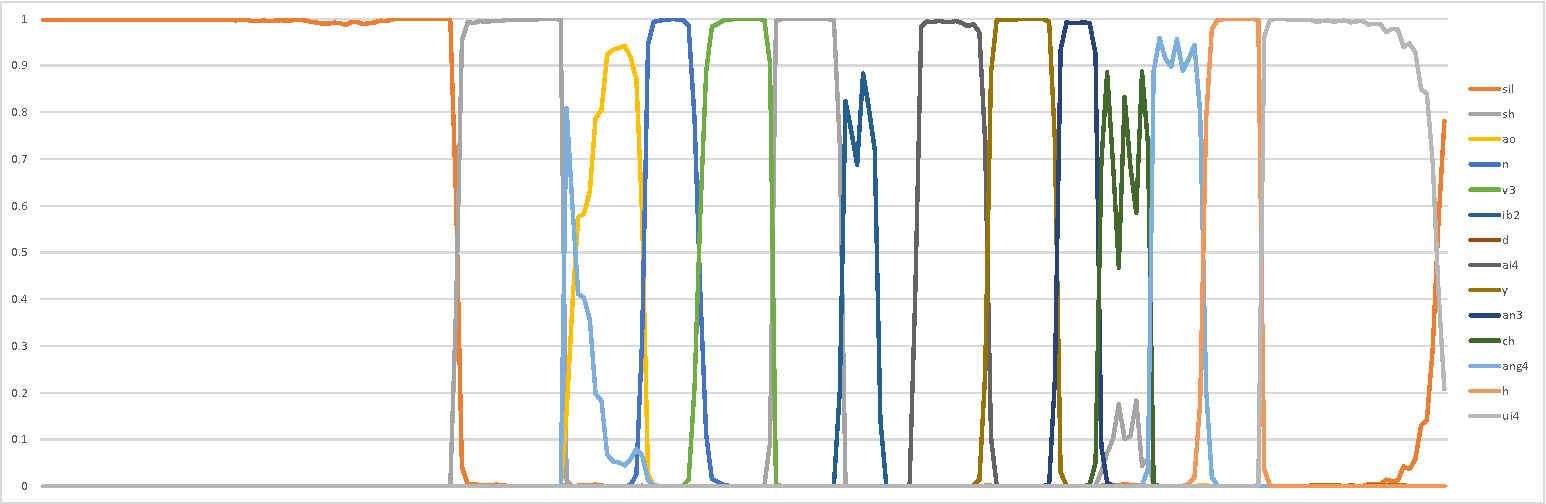
\includegraphics[width=1.0\textwidth]{figures/chapter4/ce-crop}}
  \hspace{1in}
  \subfigure[CTC Peak预测]{
    \label{fig:ctc-predict} %% label for second subfigure
    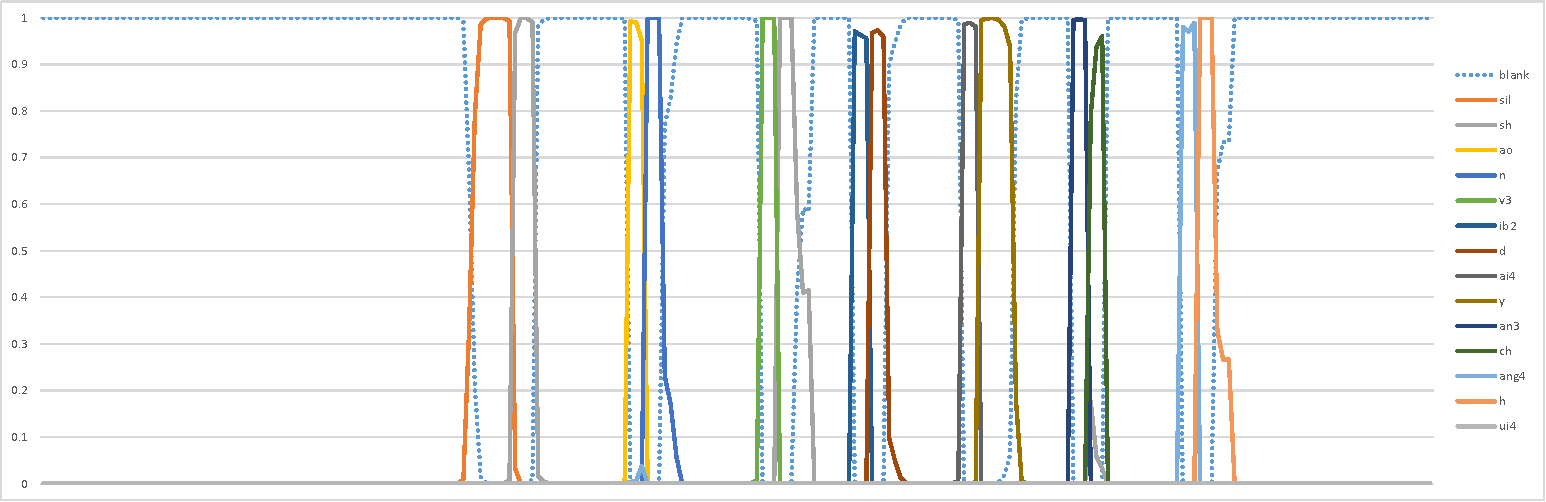
\includegraphics[width=1.0\textwidth]{figures/chapter4/ctc-crop}}
  \caption{CE和CTC预测比较}
  \label{fig:predict} %% label for entire figure
\end{figure}

图\ref{fig:predict}中给出交叉熵CE和CTC预测对比图。
可以看出,CE预测比较平滑,它在字符对应的特征区间(即对齐)内预测都趋向于1,
某些区间内还会存在混叠即竞争,表明该区间内在这些竞争字符上的概率都很高。
CTC的预测呈尖峰状,并且在大部分时刻上均输出blank,
在字符区间对应的特征上仅输出一个尖峰或者类尖峰,
在该区间上竞争字符的概率也要远远低于主字符。
即是说,CTC的Peak预测更鲁棒,区分性更好。


\subsection{CTC声学模型权重}

基于CTC的语音识别解码中,需要对语言模型和声学模型的权重进行调节,以期更好的识别结果。
使用表\ref{table:ctc}以Phone为建模单元的CTC模型CLDNN\_CTC\_Phone216(1CNN+2DNN+2LSTMP)为基础模型进行声学模型权重调节,
得到表\ref{table:ctc}结果。

\begin{table}[htbp]
\centering
\caption{CTC声学模型权重调节}
\fontsize{10.5pt}{10.5pt}\song \vspace{0.5em}
\begin{tabularx}{\textwidth}{YY}
\toprule
声学模型权重        & CER           \\ \midrule
0.50          & 9.20          \\
0.55          & 8.82          \\
0.58          & 8.71          \\
0.60          & 8.60          \\
0.63          & 8.54          \\
\textbf{0.65} & \textbf{8.53} \\
0.70          & 8.68          \\ \bottomrule
\end{tabularx}
\label{table:ctc}
\end{table}

在\ref{table:ctc}中,当声学模型权重为0.65时,基于Phone的CTC声学模型取得最佳识别结果。
而在CD-State的语音识别解码中,最佳模型的声学模型权重仅为0.06667。
可以看出,基于Phone和CTC的声学模型权重相比CD-State的模型提高了近10倍。
这得益于CTC的Peak预测特性,提高了声学模型在识别系统中的比重。

\subsection{blank打分调节}

基于CTC的声学模型在预测时,blank的打分很强,所以要对blank打分进行预处理,然后进一步进行识别解码。
本实验中先统计插入blank后的训练数据标注的先验,在得到CTC的打分之后,先减去各个字符的先验(log域),
然后再对blank打分进行调整(同样是减去某个值)。
同样使用表\ref{table:ctc}以Phone为建模单元的CTC模型CLDNN\_CTC\_Phone216(1CNN+2DNN+2LSTMP)为基础模型,
经过该处理,得到表\ref{table:blank}的结果。

\begin{table}[htbp]
\centering
\caption{CTC blank打分调节}
\fontsize{10.5pt}{10.5pt}\song \vspace{0.5em}
\begin{tabularx}{\textwidth}{YY}
\toprule
blank scale & CER           \\ \midrule
-2.0        & 8.79          \\
-1.0        & 8.54          \\
-0.5        & 8.56          \\
\textbf{0}  & \textbf{8.53} \\
0.5         & 8.62          \\
1.0         & 8.73          \\
2.0         & 9.26          \\ \bottomrule
\end{tabularx}
\label{table:blank}
\end{table}

可以看出,对blank打分进行scale操作对最终识别结果影响很大。
在该处理中,blank的先验很高,减先验相当于已经进行过scale。
所以再scale效果不是很明显,scale为0时效果最好。
如若不进行减先验处理,则scale效果会比较明显。

\subsection{CTC解码效率}

本节研究CTC的解码效率,研究CTC的Peak预测特性在语音识别解码中的作用。
本实验中,同样使用表\ref{table:ctc}的CD-States的CLDNN模型
和以Phone为建模单元的CE和CTC模型。

本实验中,使用CLDNN基础模型采用Copy模式解码。
在测试中,使用预先提好特征的测试集test3000。
对整个测试集进行解码,并统计解码的实时率RTF(Real Time Factor,解码时间与语音时长的比值)。
实验所用环境为Dell刀片式服务器,64位Ubuntu系统,24核CPU(4801MIPS),128G内存。
解码使用基于WFST的单线程解码(即每次仅解码一个测试语句)。
测试结果如表\ref{table:ctcrtf}所示。

\begin{table}[htbp]
\centering
\caption{CTC解码实时率}
\fontsize{10.5pt}{10.5pt}\song \vspace{0.5em}
\begin{tabularx}{\textwidth}{cYcc}
\toprule
编号         & 模型结构                                            & 参数量(M)           & RTF               \\ \midrule
1          & CLDNN\_CdState5389(1CNN+2DNN+2LSTMP)            & 13.81          & 0.88          \\
2          & CLDNN\_CE\_Phone216(1CNN+2DNN+2LSTMP)               & 11.15          & 1.50           \\
\textbf{3} & \textbf{CLDNN\_CTC\_Phone216(1CNN+2DNN+2LSTMP)} & \textbf{11.1567} & \textbf{0.25} \\ \bottomrule
\end{tabularx}
\label{table:ctcrtf}
\end{table}

基于深度神经网络的语音识别解码中的主要计算量有两部分,第一部分为深度神经网络的前向计算;
第二部分为识别中的Viterbi Search和Beam Search的时间。
如表\label{table:ctcrtf}所示,基于CTC的解码仅为CE模型CLDNN\_CdState5389的三分之一左右,解码速度非常快。
表中同样列出CLDNN\_CE\_Phone216模型的解码时间,其与CLDNN\_CTC\_Phone216(1CNN+2DNN+2LSTMP)模型的前向计算时间相同,
但其解码速度更慢(可能原因是其输出单元少,预测更为平滑,区分性不强)。
对比该项,即可说明CTC在解码中的优势,其Peak预测特性可以更早的裁剪竞争路径,在更早的时间减小了搜索空间,
这是CTC解码相对于CE解码的核心优势。

\begin{figure}[htbp]
\centering
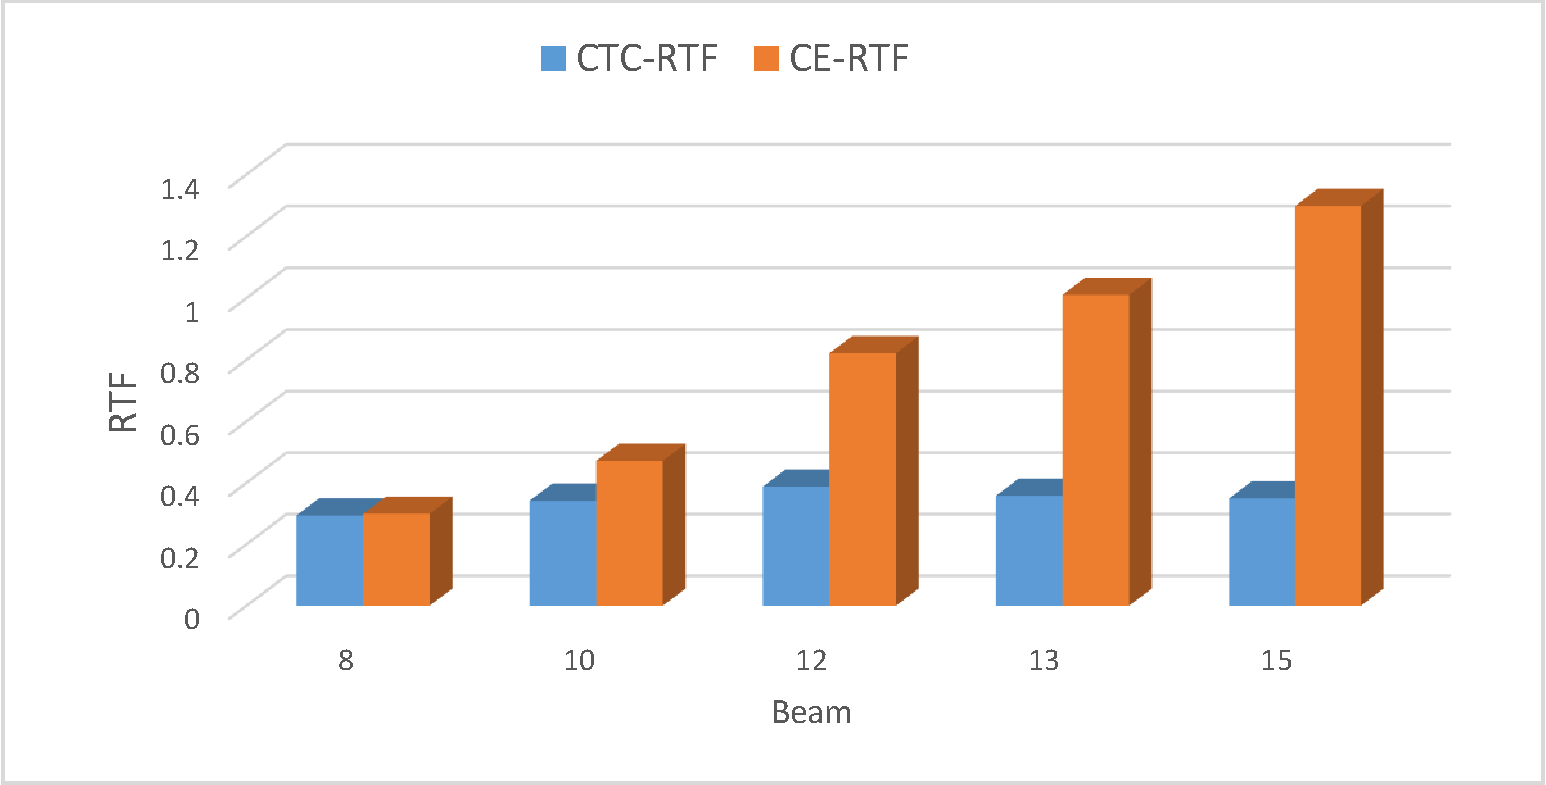
\includegraphics[width=0.6\textwidth]{figures/chapter4/beam-crop}
\caption{CTC和CE Beam对RTF影响}
\label{fig:beam}
\end{figure}

更进一步,本节给出语音识别解码Beam Search的Beam设定对CE和CTC解码的影响。
Beam是一个阈值,在语音识别解码中,
假设某条竞争路径与目前最优路径的打分之差大于该阈值,则该竞争路径即被裁剪,以及时的减小搜索空间。
所以Beam越大,搜索空间越大,语音识别的结果越好,但同时搜索时间也越久,识别时间越长。
最终结果如表\ref{table:ctcbeam}所示,进一步表示为图\ref{fig:beam}。


\begin{table}[htbp]
\centering
\caption{CTC和CE Beam对RTF影响}
\fontsize{10.5pt}{10.5pt}\song \vspace{0.5em}
\begin{tabularx}{\textwidth}{Ycccc}
\toprule
System                                                       & 参数量(M)                   & Beam & CER   & RTF      \\ \midrule
\multirow{5}{*}{CLDNN\_CTC\_Phone216(1CNN+2DNN+2LSTMP)} & \multirow{5}{*}{11.1567} & 8.0  & 11.34 & 0.29 \\
                                                             &                          & 10.0 & 10.41 & 0.34  \\
                                                             &                          & 12.0 & 10.22 & 0.38 \\
                                                             &                          & 13.0 & 9.99  & 0.35  \\
                                                             &                          & 15.0 & 9.75  & 0.34 \\ \midrule
\multirow{5}{*}{CLDNN\_CdState5389(1CNN+2DNN+2LSTMP)}        & \multirow{5}{*}{13.8104} & 8.0  & 9.34  & 0.29 \\
                                                             &                          & 10.0 & 8.76  & 0.47 \\
                                                             &                          & 12.0 & 8.63  & 0.82 \\
                                                             &                          & 13.0 & 8.63  & 1.01   \\
                                                             &                          & 15.0 & 8.64  & 1.29  \\ \bottomrule
\end{tabularx}
\label{table:ctcbeam}
\end{table}

分析可知,CTC解码实时率受Beam影响较小,而普通CE模型解码实时率RTF则严重依赖于beam大小。
因此,在CTC解码时,在保证RTF在可接受范围内的情况下,可以通过进一步放大Beam来提升模型精度。

\subsection{更大的数据}

在上述实验中,以CD-Phone为建模单元的声学模型并未取得理想的效果,期望的CD-Phone的模型效果应该优于Phone。
根据CD-Phone的聚类原理,经分析可能的原因是数据量少CD-Phone聚类不够准确导致的。

\begin{table}
\centering
\caption{CTC解码实时率}
\fontsize{10.5pt}{10.5pt}\song \vspace{0.5em}
\begin{tabularx}{\textwidth}{Ycc}
\toprule
模型                                & 建模单元数          & WER                      \\ \midrule
1CNN+9DNN(CD-State)               & 21046          & 34.9                     \\
1CNN+3LSTM(CD-Phone)              & 12167          & 32.04(8.18\%)          \\
\textbf{1CNN+3LSTM+CTC(CD-Phone)} & \textbf{12167} & \textbf{27.20(22.06\%)} \\ \bottomrule
\end{tabularx}
\label{table:bdctc}
\end{table}

因此在更大的数据集上,进行以CD-Phone为建模单元的实验。
本实验中使用百度(实习工作)2700小时的口语数据集,测试集为1500句。
其中CD-States共21046个,CD-Phone共12167个。
CD-State和CD-Phone均使用近万小时的数据聚类得到。
在该数据集上,得到表\ref{table:bdctc}的结果。


在该口语数据集上,CD-State的CLDNN效果并没有CNN基线系统的效果好,因此表\ref{table:bdctc}中没有给出CD-State的CLDNN的结果。
分析可知,基于CD-Phone的CE建模比基线CNN系统提升8.18\%,之后继续CTC训练,
最终比基线系统提升22.06\%,一方面说明了以CD-Phone作为基本建模单元的有效性,
另一方面说明CTC训练可以带来进一步的模型提升。


% !Mode:: "TeX:UTF-8"
\chapter{深度学习的并行训练}

并行化和分布式计算一直是大规模机器学习中一个让人兴奋的话题, 特别是今天,越来越多的数据被应用到深度神经网络的训练中, 对训练速度提出了很高的要求。
例如,1000h的语音数据的复杂模型(LSTM, BLSTM)训练单卡需要一周左右的时间,而上万小时的数据则需迭代数月才能完成。

而深度学习依赖于大量数据,一般数据量越大,数据覆盖的范围越广,深度学习模型的效果越好。
因此,数据对于深度学习的重要性不言而喻。
海量的训练数据,对深度学习的训练速度提出了更高的要求。
在实际应用中,使用多机多卡(GPU)的解决方案加速深度学习的训练。

主流的深度学习的并行训练大致可以分为两类,基于模型的并行和基于数据的并行。
基于模型的并行,每个Worker分到模型的不同部分,仅负责对局部模型参数的更新,类似Hogwild!\ucite{recht2011hogwild}方法。
数据并行则是将数据分成多份,分别在不同Worker上处理不同的数据,适于大量数据和较小模型的训练方式。

另外一个分类方法是根据模型更新方法可以分为两类,基于梯度的模型更新和直接基于模型的更新。
基于梯度的模型更新,Server的模型更新依赖于梯度计算,如DownpourSGD\ucite{dean2012large}(既DistBelief)和ASGD。
基于模型的更新,Server和Worker的模型更新直接基于模型,通过模型之间的计算更新,如 BSP(Model Average)、EASGD和BMUF等。

本文实现基于MPI(Message Passing Interface) 的BSP、ASGD,EASGD,BMUF四种并行方法。
四种方法均是基于数据并行的方法。
BSP,EASGD和BMUF是基于模型的方法,ASGD是基于梯度的方法。
本章介绍MPI及这四种并行基本原理和实现。

\section{MPI并行计算}

MPI是一个标准化的、可移植的消息传递协议。
它由工业界和学术界联合制定,设计了一组可以在异构计算机集群上进行并行计算的接口。
并且,MPI是跨语言的通讯协议,支持多种语言用于编写并行计算机。支持点对点和广播。
MPI协议包括协议和和语义说明,指明其如何在各种实现中发挥其特性。
MPI的目标是高性能,大规模性,和可移植性。MPI在今天仍为高性能计算的主要模型。
MPI有多种实现,例如MPICH,OpenMPI\ucite{gabriel2004open}等。

深度学习的并行实现需要在多机多卡之间进行通信。
本文选用MPI作为底层通信协议,本文使用OpenMPI的MPI实现。
本文中使用的MPI的基本接口如表\ref{table:mpi}所示。

%\begin{table}
%    \begin{tabular}{ll}
%    MPI Function    & 作用                 \\
%    MPI\_Init       & MPI初始化             \\
%    MPI\_Comm\_rank & 获取MPI的rank id      \\
%    MPI\_Comm\_size & MPI节点总数            \\
%    MPI\_Allreduce  & MPI所有节点都进行reduce操作 \\
%    MPI\_Send       & MPI发送消息            \\
%    MPI\_Recv       & MPI接收消息            \\
%    \end{tabular}
%\end{table}

\begin{table}[th]
	\centering
	\caption{本文使用的MPI的基本接口及其作用}
	\fontsize{10.5pt}{10.5pt}\song \vspace{0.5em}
	\begin{tabularx}{\textwidth}{*2{>{\centering\arraybackslash}X}@{}}
		\toprule
    MPI Function    & 作用                 \\
		\midrule
    MPI\_Init       & MPI初始化             \\
    MPI\_Comm\_rank & 获取MPI的rank id      \\
    MPI\_Comm\_size & MPI节点总数            \\
    MPI\_Allreduce  & MPI所有节点都进行reduce操作 \\
    MPI\_Send       & MPI发送消息            \\
    MPI\_Recv       & MPI接收消息            \\
		\bottomrule
	\end{tabularx}
	\label{table:mpi}
\end{table}




\section{模型平均BSP}

BSP(Bulk Synchronize Parallel),或者称之为模型平均。
其基本思路十分简单,在训练过程中,每隔一段时间对所有Worker上的模型进行同步,
同步的模型是取所有Worker上的模型平均作为更新后的新模型。
假设$w_i$表示同步前每个Worker上的模型,
$\tilde w $表示同步后的模型,$N$为Worker总数。则:
\begin{equation}
\tilde w = \frac{1}{N}\sum\limits_{i = 1}^N {{w_i}}
\end{equation}
基于BSP的并行训练的算法描述如算法\ref{alg:bsp}所示。

\begin{algorithm}
\label{alg:bsp}
\caption{BSP模型平均}
\begin{algorithmic}
\REQUIRE 同步周期$\tau$,学习率$\eta$ 
%\ENSURE

\textbf{Initial:} $\tilde w$随机初始化,$t_i=0, w_i=\tilde w$,$w_i$表示第$i$个Worker上的模型。
\REPEAT
\FOR{$i\in 1,...,N$,\textbf{parallel}}
\STATE 初始化局部模型$w_i = \tilde w$
\STATE 在$\tau$更新周期内,使用本地数据, 利用SGD更新$w_i$
\STATE ${w_i} = {w_i} - \eta \nabla w_i)$, $\nabla w_i$表示Worker$i$在$t_i$时刻由训练样本的计算梯度。
\ENDFOR
\STATE 更新全局模型: $\tilde w = \frac{1}{N}\sum\limits_{i = 1}^N {{w_i}}$
\STATE ${t_i} = {t_i} + 1$
\UNTIL{(所有样本被处理完)}
\end{algorithmic}
\end{algorithm}

基于MPI的BSP算法实现如图\ref{fig:bsp}所示,使用MPI\_Allreduce函数进行Worker间的同步通信。
当到达同步周期时,所有Worker将模型从GPU卡显存复制到CPU的内存中,并除以N,
然后同时调用MPI\_Allreduce函数的SUM操作即可。

\begin{figure}[htb]
\centering
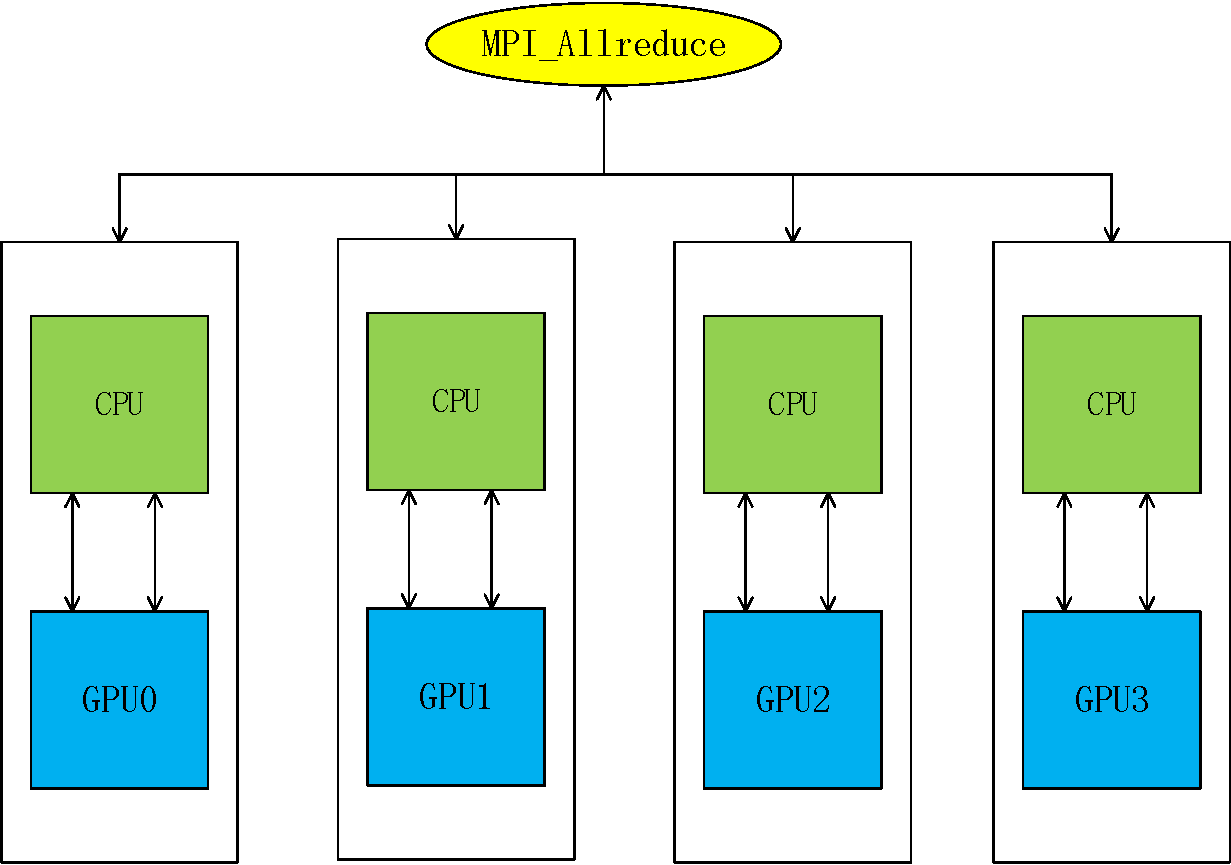
\includegraphics[width=0.5\textwidth]{figures/chapter5/bsp-crop}
\caption{基于MPI的BSP实现}
\label{fig:bsp}
\end{figure}

\section{异步随机梯度下降ASGD}

随机梯度下降SGD(Stochastic Gradient Descent)是深度学习优化的基本原理,
异步随机梯度下降ASGD(Asynchronous SGD)则是随机梯度下降的并行分布式版本。
如图\ref{fig:asgd},ASGD的深度学习系统由两部分组成:
    \begin{enumerate}
        \item 参数服务器Server,负责整体模型的存储和更新。参数服务器Server接收计算节点Worker求得的梯度,
              更新Server上的模型,并把更新后的模型发送给Worker。
        \item $N$个计算节点Worker,Worker根据本地的模型和数据计算出梯度后,将梯度发送给参数服务器,
             并从参数服务器接收最新的模型。
    \end{enumerate}

\begin{figure}[htb]
\centering
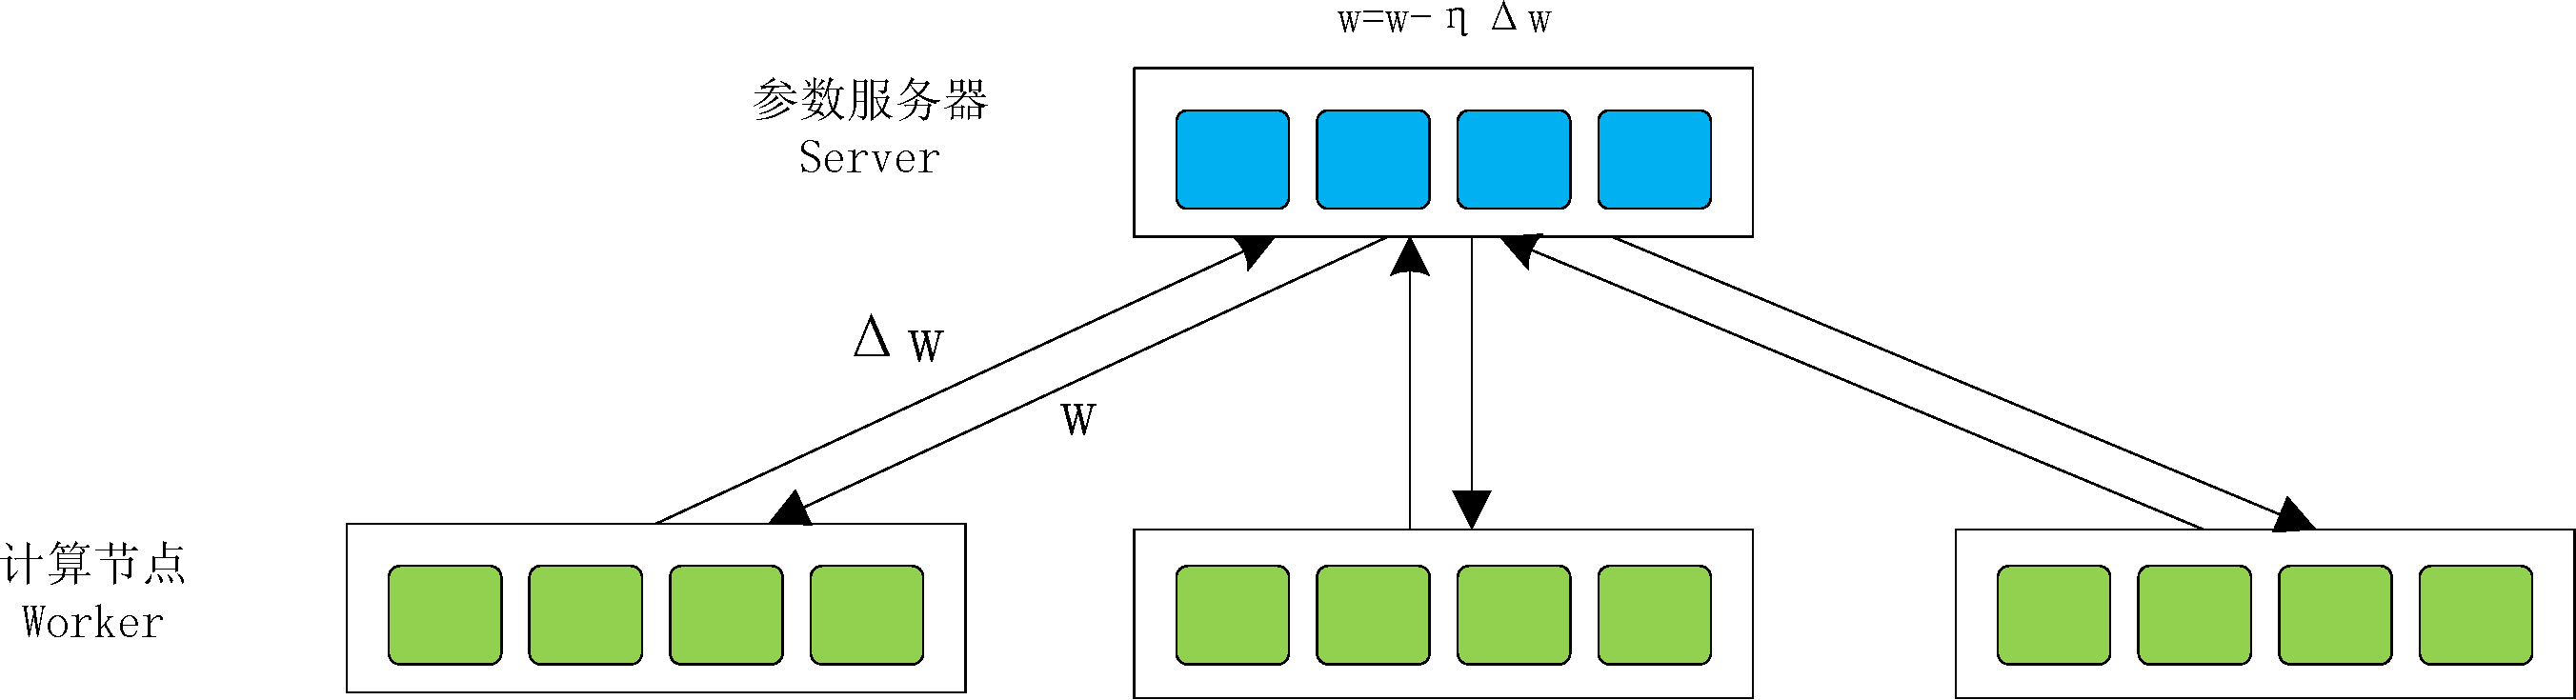
\includegraphics[width=1.0\textwidth]{figures/chapter5/asgd-crop}
\caption{异步梯度下降ASGD}
\label{fig:asgd}
\end{figure}

由图\ref{fig:asgd}可以看出,梯度是在Worker的本地模型上计算得出的梯度,
该梯度最终更新在Server的模型上,计算梯度和梯度更新的并不是同一个模型,所以
称之为异步随机梯度下降。其中Server模型的更新公式为:
\begin{equation}
{\tilde w} = {\tilde w} - \eta \nabla w_i
\end{equation}
其中$\eta$为学习率,$\nabla w_i$为当前Worker上计算发送的梯度。


在ASGD中,各个Worker独立计算,相互之间并不需要通信和同步。
每个Worker均独立和Server进行通信和模型同步,当通信和模型同步频繁时,
Server则会成为系统的性能瓶颈。
在实际应用中,同样会设定一个同步周期$\tau$,Worker计算在该周期内的累加梯度,
然后进行上述更新。$\tau$通过参数调节进行控制,$\tau$越大,Worker更新的频次越低,
系统消耗在模型等待和传输上的时间越少,系统加速的性能越好,但模型的整体效果会越差;
$\tau$越小,更新频次越高,异步程度会降低,模型效果会更好,收敛性更好,
但频繁的模型更新会导致频繁的模型同步,系统的加速性能会下降。
所以,最终同步周期$\tau$的选取则需在模型效果和加速比之间折中。

ASGD中另外一个常用的技巧是设定一个更大的全局同步周期,在该时间节点上时,
将所有Worker和Server上的模型同步为一致。
这样可以防止了各个Worker独立更新导致模型容易发散的问题,
实际应用中,我们发现采用这个技巧后模型的收敛性会更好。

\section{弹性平均随机梯度下降EASGD}

在EASGD\ucite{zhang2015deep}(Elastic Averaging SGD)中,定义优化目标为:
\begin{equation}
\label{equation:easgd}
\mathop {\min }\limits_w F(w) = \sum\limits_{i = 1}^N {f({\rm{S|}}{w_i})} {\rm{ + }}\frac{\lambda }{2}{\rm{||}}{w_i} - \tilde w|{|^2}
\end{equation}
其中$S$代表训练集,$f(.)$代表单卡的神经网络的优化目标,即训练的损失函数,可以是交叉熵CE,最小均方差MSE等的优化准则。
$\lambda$是可调的权重参数,$w_i$表示每个Worker上的模型,$\tilde w $表示Server上的模型。

所以,EASGD的优化目标为使所有Worker上的损失最小,并且各个Worker与Server之间的模型差异也要小, 这样把Worker节点上的参数跟参数服务器的中心变量联系在一起,这样使得Worker本地的模型会围绕中心Server上的模型进行变化。
上面提到,在ASGD中通过设定全局同步周期来防止各个Worker独立计算导致的模型容易发散的问题,
EASGD中则直接通过形式化的方法来达到该目标,$\frac{\lambda }{2}{\rm{||}}{w_i} - \tilde w|{|^2}$类似一个正则项,
强制Worker上的模型围绕Server上的模型进行优化。
$\lambda$比较大时,正则因子越强,Worker的模型倾向于利用当前的Server模型进行优化,
$\lambda$比较小时,正则因子越小,Worker倾向于在当前Server模型的基础上进行更多的探索。

式\ref{equation:easgd}对$\tilde w$和$w_i$进行求导有:
\begin{equation}
\begin{array}{l}
{w_i} = {w_i} - \eta \nabla {w_i} - \eta \lambda ({w_i} - \tilde w)\\
\tilde w = \tilde w - \eta \lambda \sum\limits_{i = 1}^N ( \tilde w - {w_i})
\end{array}
\end{equation}
这是同步的EASGD的更新公式。

在异步的EASGD中,略去Worker自身局部梯度$\nabla {w_i}$,略去同步,令$\alpha  = \eta \lambda$,
则单个Worker对Server模型的更新公式为:
\begin{equation}
\begin{array}{l}
{w_i} = {w_i} - \alpha ({w_i} - \tilde w)\\
\tilde w = \tilde w - \alpha (\tilde w - {w_i})
\end{array}
\end{equation}
$\alpha$控制模型的更新步长。

本文实现并使用异步的EASGD,该算法描述如算法\ref{alg:easgd}所示:
\begin{algorithm}
\label{alg:easgd}
\caption{异步EASGD}
\begin{algorithmic}
\REQUIRE 同步周期$\tau$,学习率$\alpha$ \\
%\ENSURE
\textbf{Initial:} $\tilde w$随机初始化,$t_i=0, w_i=\tilde w$,$w_i$表示第$i$个Worker上的模型。
\REPEAT
\STATE 训练数据样本$s$
\STATE $w=w_i$(中间变量)
\IF{($\tau$整除$t_i$)}
\STATE ${w_i} = {w_i} - \alpha ({w} - \tilde w)$
\STATE $\tilde w = \tilde w - \alpha (\tilde w - {w})$
\ENDIF
\STATE ${w_i} = {w_i} - \eta \nabla w_i(s)$, $\nabla w_i(s)$表示Worker$i$在$t_i$时刻由样本$s$的计算梯度。
\STATE ${t_i} = {t_i} + 1$
\UNTIL{(所有样本被处理完)}
\end{algorithmic}
\end{algorithm}

\section{BMUF} 

2016年,微软在语音识别任务上提出BMUF\ucite{chen2016scalable}(Block Momentum Update Filtering)并行算法,
并在语音识别任务上取得不错的加速比和更优的模型精度。

BMUF算法同样基于模型。
在训练的一次更新中,首先广播上一时刻的全局模型$\tilde w$到所有Worker,Worker利用$\tilde w$初始化自身模型$w_i$即:
\begin{equation}
w_i = \tilde w
\end{equation}
并在自身的数据上迭代更新$w_i$。

到达同步周期后,需要更新全局模型$\tilde w$。
在BMUF中,使用学习的方法进行更新,即计算梯度,设定学习率,利用梯度方法进行更新。
第$i$个Worker上的梯度为:
\begin{equation}
\nabla {w_i} = {w_i} - \tilde w
\end{equation}
所有Worker上的梯度和为:
\begin{equation}
\nabla {{\tilde w}_t} = \nabla {{\tilde w}_{t - 1}} + \varepsilon \sum\limits_{i = 1}^N {\nabla {w_i}}
\end{equation}
其中$\varepsilon$为冲量Momentum,类似SGD中的冲量。
则全局模型的更新为:
\begin{equation}
\tilde w = \tilde w - \eta \nabla {{\tilde w}_t}
\end{equation}

\begin{algorithm}
\label{alg:bmuf}
\caption{BMUF}
\begin{algorithmic}
\REQUIRE 同步周期$\tau$,学习率$\eta$,冲量$\varepsilon$ \\
%\ENSURE

\textbf{Initial:} $\tilde w$随机初始化,$t_i=0, w_i=\tilde w$,$w_i$表示第$i$个Worker上的模型。
\REPEAT
\FOR{$i\in 1,...,N$,\textbf{parallel}}
\STATE 初始化局部模型$w_i = \tilde w$
\STATE 在$\tau$更新周期内,使用本地数据, 利用SGD更新$w_i$
\STATE 计算$\nabla {w_i} = {w_i} - \tilde w$
\ENDFOR
\STATE 收集所有Worker的梯度,并加冲量:
    $\nabla {{\tilde w}_t} = \nabla {{\tilde w}_{t - 1}} + \varepsilon \sum\limits_{i = 1}^N {\nabla {w_i}}$
\STATE 更新全局模型: $\tilde w = \tilde w - \eta \nabla {{\tilde w}_t}$
\UNTIL{(所有样本被处理完)}
\end{algorithmic}
\end{algorithm}

BMUF的算法描述如算法\ref{alg:bmuf}所示。
可以简单比较一下BSP和BMUF。两者在算法的流程上一致,不同之处在于全局模型的更新策略,
BSP中直接取模型平均作为新的模型,而BMUF中则根据梯度进行学习更新,并且引入Momentum加速学习的速率。

同样,简单比较一下EASGD和BMUF。两者在均是基于模型的并行方法,
更新时同样需要计算全局模型和局部模型之间的差分,然后使用该差分更新模型。
不同之处在于:
\begin{enumerate}
\item BMUF是全局同步的方法,每一次更新之后,所有的Worker均使用相同的初始模型;
\item BMUF的差分中引入类似SGD学习中的冲量,而冲量可以加速模型的收敛。
\end{enumerate}
\include{body/conclusion}


%% 参考文献
\defaultfont
\bibliographystyle{ref/GBT7714-2005}
\addcontentsline{toc}{chapter}{参考文献}              % 参考文献加入到中文目录
\addcontentsline{toe}{chapter}{\bfseries References} % 参考文献加入到英文目录
\addtolength{\bibsep}{-0.8em}
\nocite{*}  %若将此命令屏蔽掉,则未引用的文献不会出现在文后的参考文献列表中。
\bibliography{ref/ref}
\clearpage\mbox{}

% \include{appendix/appA}           % 附录
%% !Mode:: "TeX:UTF-8" 

\BiAppendixChapter{致\quad 谢}{Acknowledgements}
回首一瞥,我在XXXX大学的学习生活已经步入了第十个春秋。今年也是我博士学习的第六个年头,终于走了毕业的门槛处。回思在XXX所度过的我最为青春的十年岁月,胸中所填满的思绪远远不是一张纸可以倾诉得尽。相比于比较浑浑噩噩的本科生活,六年的博士学习生活已经在我成长的历程中留下了各种印记。我的价值观也基本是在这六年里被塑造定型,更为重要的是我的研究习惯和思维模式也在师长和同窗的帮助下逐渐修成。值此即将跨过博士毕业的门槛之际,我想向那些在这段岁月里陪我成长的人表达我最深的谢意。

首先我最想表达的是对父母和兄长的谢意以及歉意。谢谢家人们一直在我背后的角落里默默的支持着我。一直以来,因为在学业上的长久投入,常常忽略了我身后的家人们。作为儿子没有向父母尽我应有的孝道,作为幼弟没有帮助兄长操持这个家庭。在这里我想对我最亲的家人们说出最深的对不起,儿在此遥拜远方的双亲。

衷心感谢我的导师XXX教授和XX教授一直以来对我博士学业的督导和促进。当初若非蒙受X老师的引导,我或将长久地迷茫徘徊于科研门外。您身上对工作的热情和对研究的激情从一开始就深深地感染着我的成长。在您的所有学生中,我的天资平庸,勤奋度上一直也做的不好,感谢X老师一直以来对我不懈的循循劝导,并为我提供了众多促我成长的机会。在实验室的日子里,虽然会忙一些累一点,但如今回头看去这些点点滴滴确实对我的成长具有莫大的助益。再次感谢恩师六年的栽培之恩!

感谢XX老师在我转换了研究方向之后的博士后半程对我的博士学业所提供的无私的帮助。若非蒙XX老师后期的提携助益,我的博士研究工作定会多走许多弯路。感谢XXX老师和XXX老师在我博士期间提供的无私帮助。感谢我在英国访学期间XXX教授和XXX老师对我的关照和指导。

感谢我刚加入这儿实验室时,帮助我入门,并不厌其烦地对我的诸多困惑进行耐心解答的诸多师兄师姐们。感谢XXX、XXX等众师姐师兄等对刚入门时的我的关怀和帮助。感谢XXX师兄、XXX师姐在我成长中提供的兄长与姐姐般的关怀。感谢实验室的一班亲如兄弟姐妹的师弟师妹们,正因有了你们的一路陪伴,我的六年读博生活也就不再那么苦涩难熬了。衷心感谢有这么多的同窗好友们的一路陪伴:XXX、XXX、XXX、XX、XXX、XXX、XXX、XXX、XXX、XXX、XXX等等。感谢我的女朋友XXX为我枯燥的博士研究生活带来了一种满含温情的情调,原来生活还可以过得如此不同。

最后,再次感谢我的家人、实验室各位师长和众位同窗们,谢谢你们的一路陪伴!

\quad\quad\quad\quad\quad\quad\quad\quad\quad\quad\quad\quad\quad\quad\quad\quad\quad\quad\quad\quad\quad\quad\quad\quad\quad\quad\quad\quad\quad\quad XXX

\quad\quad\quad\quad\quad\quad\quad\quad\quad\quad\quad\quad\quad\quad\quad\quad\quad\quad\quad\quad\quad\quad\quad\quad\quad\quad\quad\quad\quad 2016年1月

%衷心感谢导师~XXX~教授对本人的精心指导。他的言传身教将使我终生受益。感谢~XXX~教授,以及实验室全体老师和同窗们的热情帮助和支持!本课题承蒙~XXXX~基金资助,特此致谢。



\clearpage\mbox{}
 % 致谢
% !Mode:: "TeX:UTF-8"

\BiAppendixChapter{致\quad 谢}{Acknowledgements}

\vspace{2ex}
岁月如白驹过隙,硕士转瞬即尽,彷徨过,迷惘过,有过辛酸,有过汗水,也有些许成就。
在技术上,三年的教研室的科研生涯使我的科研和工程能力得到进一步提高,能够独当一面;通过外出实习,个人视野更加的广阔,
对个人研究方向在工业界的大规模应用有了更清晰的认识,更好的把握时代的前沿科技。
在生活上,自信而自律,文艺而又不失洒脱,能够在生活和工作上找到自己的平衡点。


首先,特别感谢我的导师谢磊教授。谢老师视野开阔,工作勤奋,对新的技术和事物有着很强的把握;
孜孜不已,诲人不倦,以身做则,才有如今“谢家桃李满天下”;他的勤奋和努力始终鼓舞着我。
在科研工作上,谢老师经常与我们共同讨论,提出自己的想法和意见。在实习工作上,谢老师主动努力为我们提供更好的
实习和工作机会。

感谢实验室的各位同学,感谢那些与你们一起科研,一起Happy,一起疯狂的日子。

感谢我的诸位室友,谢谢你们的陪伴与互勉,让我三年的研究生生涯异样的精彩。

当然,从前种种譬如昨日之死,以后种种譬如今日之生。这又是人生的新起点!


\quad\quad\quad\quad\quad\quad\quad\quad\quad\quad\quad\quad\quad\quad\quad\quad\quad\quad\quad\quad\quad\quad\quad\quad\quad\quad\quad\quad\quad\quad 张彬彬

\quad\quad\quad\quad\quad\quad\quad\quad\quad\quad\quad\quad\quad\quad\quad\quad\quad\quad\quad\quad\quad\quad\quad\quad\quad\quad\quad\quad\quad 2017年3月

%衷心感谢导师~XXX~教授对本人的精心指导。他的言传身教将使我终生受益。感谢~XXX~教授,以及实验室全体老师和同窗们的热情帮助和支持!本课题承蒙~XXXX~基金资助,特此致谢。



\clearpage\mbox{}
 % 致谢
%% !Mode:: "TeX:UTF-8" 

\defaultfont
\BiAppendixChapter{攻读\cxuewei 学位期间发表的论文及其他成果} {Papers published in the period of PH.D. education}
\setlength{\parindent}{0em}
\textbf{一、发表的学术论文}
\begin{publist}
\item XXX. Online Object Tracking Based on BLSTM-RNN with Contextual-Sequential Labeling[C]. \textcolor{blue}{IEEE Transactions on Multimedia (TMM)} (under review).(\underline{\bf SCI 2区})
\item XXX. Tennis Ball Tracking Using A Two-layered Data Association Approach[J]. \textcolor{blue}{IEEE Transactions on Multimedia (TMM)}, 2015, 17(2): 145-156.(\underline{\bf SCI 2区})
\item XXX. Online Object Tracking Based on CNN with Metropolis-Hasting Re-sampling[C]. In \textcolor{blue}{ACM international conference on Multimedia (ACMMM)}, Brisbane, Australia, 2015: 1163-1166.(\underline{\bf CCF A类会议})
\item XXX. An Ensemble of Deep Neural Networks for Object Tracking[C]. In \textcolor{blue}{IEEE International Conference on Image Processing (ICIP)}, Paris, France, 2014: 843-847.(\underline{\bf CCF C类会议},获选大会Top10\%文章)
\item XXX. Unsupervised Broadcast News Story Segmentation Using Distance Dependent Chinese Restaurant Processes[C]. \textcolor{blue}{The 39th International Conference on Acoustics, Speech, and Signal Processing (ICASSP)}, Florence, Italy, 2014: 4062-4066.(\underline{\bf CCF B类会议})
\item XXX. A Two Layered Data Association Approach for Ball Tracking[C]. In \textcolor{blue}{IEEE International Conference on Acoustics, Speech, and Signal Processing (ICASSP)}, Vancouver, Canada, 2013: 2317-2321.(\underline{\bf CCF B类会议})
\item XXX. Detection of Ball Hits in A Tennis Game Using Audio and Visual Information[C]. In \textcolor{blue}{IEEE Asia-Pacific Signal Information Processing Association Annual Summit and Conference (APSIPA ASC)}, Hollywood, California, 2012: 1-10.
\item XXX. Real-time Speech-driven Virtual Avatar[J]. \textcolor{blue}{Journal of Tsinghua University}, 2011, 51(9): 1180-1186.(\underline{\bf NCMMSC最佳学生论文提名})
\item XXX. Speech and Auditory Interfaces for Ubiquitous, Immersive and Personalized Applications[C]. In \textcolor{blue}{Immersive and Personalized Applications, Ubiquitous Intelligence Computing and the 7th International Conference on Autonomic Trusted Computing (UIC/ATC)}, Xi’an, China, 2010: 503-505.
\end{publist}
\vspace{0.5cm}

\textbf{二、博士期间的获奖情况}
\begin{publist}
 \item ICIP 2014 Top\%10 Paper Award.({\bf 第一作者})
 \item 第10届京港国际博士生论坛Best Paper.({\bf 第一作者})
 \item 获2016年XXXX大学计算机学院“图灵之星”奖
 \item 获2015年XXXX大学“理光奖学金”
 \item 获2015年XXXX大学“海泰奖学金”
\end{publist}
% \textbf{二、参与的科研项目及获奖情况}
% \begin{publist}
% \item XX. Towards A Queue-Aware ATM: Monitoring and Managing Queues in Front of ATMs, NCR英国国际合作项目.课题编号:XXXX.
% \item XX. 语音内容分析的关键技术研究, 陕西省自然科学基础研究计划.课题编号:XXXX.
% \item XX. 基于DBN协同建模的中文及跨语种语音结构事件检测研究, 国家自然科学基金.课题编号:XXXX.
% \item XX. 机载语音处理技术,	研究所合作项目.课题编号:XXXX.
% \end{publist}
% \vfill
% \hangafter=1\hangindent=2em\noindent

% \setlength{\parindent}{2em}
\clearpage\mbox{}     % 所发文章
% !Mode:: "TeX:UTF-8"

\defaultfont
\BiAppendixChapter{攻读\cxuewei 学位期间发表的论文及其他成果} {Papers published in the period of PH.D. education}
\setlength{\parindent}{0em}
\textbf{一、发表的学术论文}
\begin{publist}
  \item {\bf Xiangzeng Zhou}, Lei Xie, Peng Zhang and Yanning Zhang. Online Object Tracking Based on BLSTM-RNN with Contextual-Sequential Labeling[C]. \textcolor{blue}{IEEE Transactions on Multimedia (TMM)} (under review).(\underline{\bf SCI 2区})
\end{publist}
\vspace{1cm}

\textbf{二、博士期间的获奖情况}
\begin{publist}
 \item ICIP 2014 Top\%10 Paper Award.({\bf 第一作者})
 \item 第10届京港国际博士生论坛Best Paper.({\bf 第一作者})
 \item 获2016年西北工业大学大学计算机学院“图灵之星”奖
 \item 获2015年西北工业大学“理光奖学金”
 \item 获2015年西北工业大学“海泰奖学金”
\end{publist}
% \textbf{二、参与的科研项目及获奖情况}
% \begin{publist}
% \item XX. Towards A Queue-Aware ATM: Monitoring and Managing Queues in Front of ATMs, NCR英国国际合作项目.课题编号:XXXX.
% \item XX. 语音内容分析的关键技术研究, 陕西省自然科学基础研究计划.课题编号:XXXX.
% \item XX. 基于DBN协同建模的中文及跨语种语音结构事件检测研究, 国家自然科学基金.课题编号:XXXX.
% \item XX. 机载语音处理技术,	研究所合作项目.课题编号:XXXX.
% \end{publist}
% \vfill
% \hangafter=1\hangindent=2em\noindent

% \setlength{\parindent}{2em}
     % 所发文章
% !Mode:: "TeX:UTF-8"

\newpage
\thispagestyle{empty}
\markboth{西北工业大学学位论文知识产权说明书}{西北工业大学学位论文原创性声明}

\vspace*{0.1cm}
%\newcommand{\subchapterstyle}%
%  {\CJKfamily{hei}\rmfamily\bfseries\fontsize{14pt}{14pt}\selectfont}

\newcommand{\subchapterstyle}{\song\bfseries\fontsize{14pt}{14pt}}
\newcommand{\twospace}{~~~~~~~~}

%\phantomsection
%\addcontentsline{toc}{chapter}{\hei\xiaosi 西北工业大学学位论文知识产权说明书}
%\addcontentsline{toe}{chapter}{\bfseries\xiaosi Statement of Copyright}
\begin{center}{\subchapterstyle 西北工业大学 \\ \vspace*{0.1cm} 学位论文知识产权说明书}\end{center}

    {\fontsize{10.5pt}{13pt}\selectfont \twospace 本人完全了解学校有关保护知识产权的规定,即:研究生在校攻读学位期间论文工作的知识产权单位属于西北工业大学。
    学校有权保留并向国家有关部门或机构送交论文的复印件和电子版。本人允许论文被查阅和借阅。
    学校可以将本学位论文的全部或部分内容编入有关数据库进行检索,可以采用影印、缩印或扫描等复制手段保存和汇编本学位论文。
    同时本人保证,毕业后结合学位论文研究课题再撰写的文章一律注明作者单位为西北工业大学。


    \twospace 保密论文待解密后适用本声明。


    \twospace 学位论文作者签名:\underline{\quad\quad\quad\quad\quad\quad\quad} \hspace{8em}指导教师签名:\underline{\quad\quad\quad\quad\quad\quad\quad}

    \hspace{5em} \quad 年 \quad 月 \quad 日 \hspace{17em} 年 \quad 月 \quad 日 \quad}





\vspace{1\baselineskip}
---------------------------------------------------------------------------------------------------------
\vspace{1\baselineskip}

%\phantomsection
%\addcontentsline{toc}{chapter}{\hei 西北工业大学学位论文原创性声明}
%\addcontentsline{toe}{chapter}{\bfseries\xiaosi Letter of Authorization}
\begin{center}{\subchapterstyle 西北工业大学 \\ \vspace*{0.1cm}学位论文原创性声明}\end{center}

 {\fontsize{10.5pt}{13pt}\selectfont \twospace 秉承学校严谨的学风和优良的科学道德,本人郑重声明:所呈交的学位论文,是本人在导师的指导下进行研究工作所取得的成果。
 尽我所知,除文中已经注明引用的内容和致谢的地方外,本论文不包含任何其他个人或集体已经公开发表或撰写过的研究成果,
 不包含本人或其他已申请学位或其他用途使用过的成果。对本文的研究做出重要贡献的个人和集体,均已在文中以明确方式表明。

\twospace 本人学位论文与资料若有不实,愿意承担一切相关的法律责任。

\vspace{0.5\baselineskip}

\hspace{14em} 学位论文作者签名:\underline{\quad\quad\quad\quad\quad\quad\quad}

\hspace{18em} \quad 年 \quad 月 \quad 日}


% \BiAppendixChapter{西北工业大学学位论文原创性声明及使用授权说明}{Statement of copyright and Letter of authorization}
% \vspace{\baselineskip}
% \begin{center}\hei\xiaosan{学位论文原创性声明}\end{center}
% \vspace{1em}

% 本人郑重声明:此处所提交的学位论文《\chinesethesistitle》,是本人在导师指导下,在哈尔滨工业大学攻读学位期间独立进行研究工作所取得的成果。据本人所知,论文中除已注明部分外不包含他人已发表或撰写过的研究成果。对本文的研究工作做出重要贡献的个人和集体,均已在文中以明确方式注明。本声明的法律结果将完全由本人承担。

% \vspace{\baselineskip}
% \hspace{6em}作者签名:\hfill 日期:\hspace{2.5em}年\hspace{1.5em}月\hspace{1.5em}日

% \vspace{3\baselineskip}
% \begin{center}\hei\xiaosan{学位论文使用授权说明}\end{center}
% \vspace{1em}

% 本人完全了解哈尔滨工业大学关于保存、使用学位论文的规定,即:

% (1)已获学位的研究生必须按学校规定提交学位论文;(2)学校可以采用影印、缩印或其他复制手段保存研究生上交的学位论文;(3)为教学和科研目的,学校可以将学位论文作为资料在图书馆及校园网上提供目录检索与阅览服务;(4)根据相关要求,向国家图书馆报送学位论文。

% 保密论文在解密后遵守此规定。
% \vspace{\baselineskip}

% 本人保证遵守上述规定。

% \vspace{2\baselineskip}
% \hspace{6em}作者签名:\hfill 日期:\hspace{2.5em}年\hspace{1.5em}月\hspace{1.5em}日

% \vspace{2\baselineskip}
% \hspace{6em}导师签名:\hfill 日期:\hspace{2.5em}年\hspace{1.5em}月\hspace{1.5em}日
    % 承诺

% \ifxueweidoctor
% \include{appendix/Resume}         % 博士学位论文有个人简介
% \fi

\clearpage

\end{document}

%%% Local Variables:
%%% mode: latex
%%% TeX-master: t
%%% End:
